% TODO: use the \Defined notation a bit more pervasively
% TODO: intro paragraph?
% TODO: search for ``paper'' everywhere and make sure it reads ``chapter''
% in the dissertation
% TODO: search for ``lack of space'' and figure out what to do about each --
% there's no lack of space in a dissertation!!
\newif \iffailed \failedfalse % to remove some bits we think we don't need
\ifdissertation\newcommand{\symmlenses}{ Chapter~\ref{chap:complement}\xspace}
\else          \newcommand{\symmlenses}{~\cite{HofmannPierceWagner10}\xspace}
\fi
\sect{Overview}
\label{sec:delta-examples}

\begin{figure}
    \begin{center}
        \vspace*{-2ex}
        
\includegraphics[width=75mm]{images/ex1-init.pdf} \\
        (a) initial \replicas \\[1.5ex]
        
\includegraphics[width=75mm]{images/ex1-1.pdf} \\
        (b) a new composer is added to one \replica \\[2ex]
        
\includegraphics[width=75mm]{images/ex1-2.pdf} \\
        (c) the lens adds the new composer to the other \replica \\[1.5ex]
        
\includegraphics[width=75mm]{images/ex1-3.pdf} \\
        (d) the curator makes some corrections \\[.8ex]
        
\includegraphics[width=75mm]{images/ex1-4.pdf} \\[-3ex]
        (e) the lens transports a small edit \\[1.5ex]
        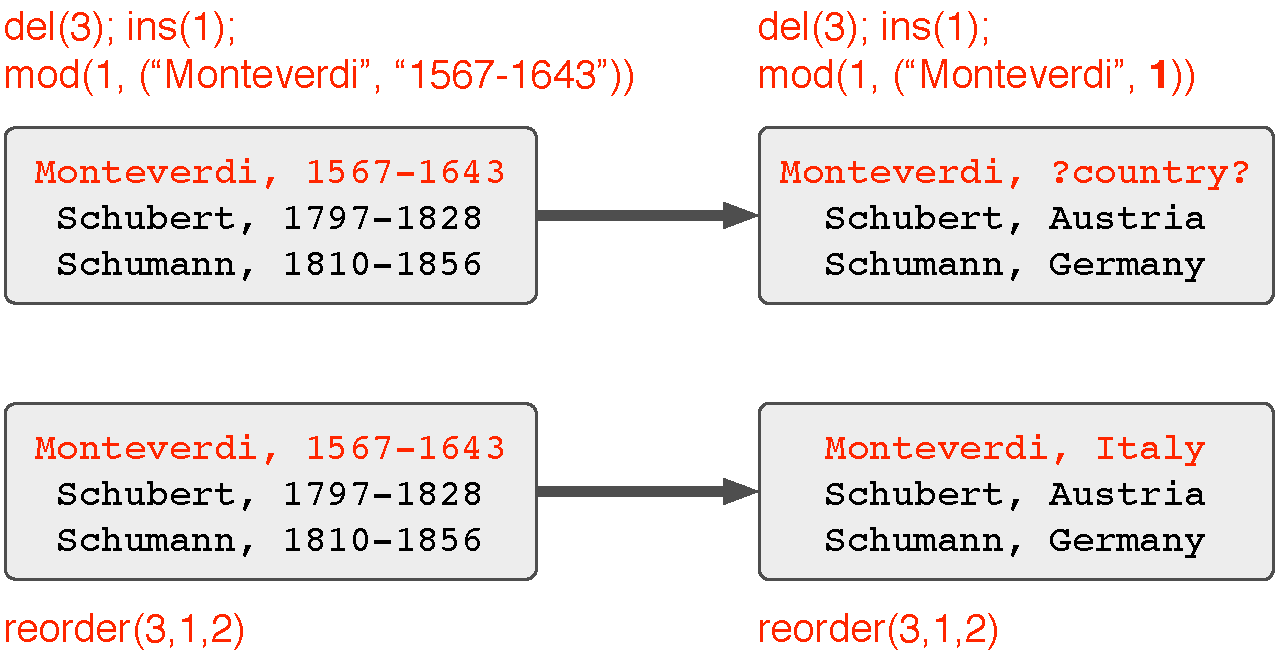
\includegraphics[width=75mm]{images/ex1-5.pdf} \\
        (f) two different edits with the same effect on the left
    \end{center}
\iflater
\discuss{Change the font everywhere to sf}
\fi
    \caption{A simple (complement-less) {\edit} lens in action.}
    \label{fig:example-simple}
\end{figure}

Before diving into \ifdissertation the technicalities of edit lenses, \else
technicalities, \fi let's take a brief tour of the main ideas via some
examples.
%
Figure~\ref{fig:example-simple} demonstrates a simple use of {\edit} lenses
to synchronize two \replicas\ifdelta\footnote{We use the word ``synchronize''
  informally to mean simply ``maintain a correspondence between two replicas
  by propagating edits in both directions.''  A full-blown synchronization
  tool would also include, at a minimum, some mechanism for dealing with
  conflicts between disconnected edits to the two structures, which is
  outside the scope of this paper.  \iffull Note, though, that we go beyond most
  synchronization tools in allowing the replicas to be structured
  differently and to share only a part of their information.\fi}\fi.  In part (a),
we see the initial \replicas, which are in a synchronized state.  On the
left, the \replica is a list of records describing composers' birth and death
years; on the right,  a list of records describing the same
composers' countries of origin.  In part (b), the user interacting with the
left-hand \replica decides to add a new composer, {\sf Monteverdi}, at the
end of the list. This change is described by the edit script {\sf ins(3);
mod(3, (``Monteverdi'', ``1567-1643''))}. The script says to first
\emph{insert} a dummy record at index three, then \emph{modify} this record by
replacing the left field with ``{\sf Monteverdi}'' and replacing the 
right field with ``{\sf 1567-1643}''.  (One could of course imagine other edit
languages where the insertion would be done in one step.  We represent it
this way because this is closer to how our generic ``container mapping''
combinator in \S \ref{sec:containers} will do things.) The lens connecting
the two \replicas now converts this edit script into a corresponding edit
script that adds {\sf Monteverdi} to the right-hand \replica, shown in part
(c): {\sf ins(3); mod(3, (``Monteverdi'', \ONE))}.
Note that the translated {\sf mod} command overwrites the name component but
leaves the country component with its default value, ``{\sf
  ?country?}\dotquote This is the best it can do, since the edit was in
the left-hand \replica, which doesn't mention countries.  
%
Later, an eagle-eyed editor notices the missing country information and
fills it in, at the same time correcting a spelling error in {\sf
  Schumann}'s name, as shown in (d). In part (e), we see that the lens
discards the country information when
translating the edit from right to left, but propagates the spelling
correction. 

Of course, a particular new \replica state can potentially be achieved by
many different edits, and these edits may be translated differently.
Consider part (f) of Figure~\ref{fig:example-simple}, where the left-hand
\replica ends up with a row for {\sf Monteverdi} at the beginning of the
list, instead of at the end. Two edit scripts that achieve this effect are
shown. The upper script deletes the old {\sf Monteverdi} record and inserts
a brand new one (which happens to have the same data) at the top; the lower
script rearranges the order of the list. The translation of the upper edit
leaves {\sf Monteverdi} with a default country, while the lower edit is
translated to a rearrangement, preserving all the information associated
with {\sf Monteverdi}.

We do not address the question of where these edits come from or who
decides, in cases like part (f), which of several possible edits is
intended.  As argued in~\cite{Matching10}, answers to these questions will
tend to be intertwined with the specifics of particular editing and/or
diffing tools and will tend to be messy, heuristic, and
domain-specific---unpromising material for a foundational theory.  Rather,
our aim is to construct a theory that shows how edits, however
generated, can be translated between \replicas of different shapes.

\iflater\finish{A lot of people got lost at this point.  We need to go much more
  gently.  (In particular, start with a roadmap.)  It would help to rename
  $X,Y,Z$ to something more mnemonic.}\fi

Abstractly, the lens we are discussing maps between structures of the form
$(X \times Y)\LIST$ and ones of the form $(X \times Z)\LIST$, where $X$ is the set
of composer names, $Y$ the set of date strings, and $Z$ the set of
countries.  We want to build it compositionally---that is, the whole lens
should have the form $\ell\LIST$, where $-\LIST$ is a ``list mapping'' lens
combinator and $\ell$ is a lens for translating edits to a
single record---i.e., $\ell$ is a lens from $X \times Y$ to $X \times Z$.
Moreover, $\ell$ itself should be built as the product $\ell_1 \times
\ell_2$ of a lens $\ell_1 \in X \to X$ that translates composer edits
verbatim, while $\ell_2$ is a ``disconnect'' lens that maps every edit on
either side to a trivial identity edit on the other side.

In analogous fashion, the edit languages for the top-level structures will
be constructed compositionally.  The set of edits for structures of the form
$(X \times Y)\LIST$, written $\partial ((X \times Y)\LIST)$, will be defined
together with the list constructor $-\LIST$.  Its elements will have the form
$\mlins{i}$ where $i$ is a position, $\mldel{i}$,
$\mlreorder{i_1,\ldots,i_n}$ where $i_1,\ldots,i_n$ is a permutation on
positions (compactly represented, e.g. as a branching program),
\iflater\discuss{people will be suspicious here---how do we know we
  can represent it compactly?}\fi and $\mlmod{p}{\dv}$, where $\dv \in
\partial (X\times Y)$ is an edit for $X \times Y$ structures.  Pair edits
$\dv \in \partial (X \times Y)$ have the form $\partial X \times
\partial Y$, where $\partial X$ is the set of edits to composers and
$\partial Y$ is the set of edits to dates.  Finally, both $\partial
X$ and $\partial Y$ are sets of primitive ``overwrite edits'' that completely
replace one string with another, together with an identity edit $\ONE$
that does nothing at all; so $\partial X$ can be just $\{\unit\} + X$ (with
$\ONE = \mlinl\unit$) and similarly for $Y$ and $Z$.

%% We write $\ONE$ instead of $\mlinl\ONE$ and {\sf
%%   ``x''} instead of $\mlinr x$ in contexts where it is clear that an edit of
%% this form is expected.

%% We can represent an edit to an element of $X \times Y$ as a pair of
%% edits to $X$ and $Y$; that is, $\partial(X \times Y) = \partial X \times
%% \partial Y$.  The application function $\odot_{X \times Y}$ simply applies
%% each of the component edits to the appropriate parts of the
%% product:
%% \iffull \[ \else $ \fi
%% (\dx,\dy) \odot_{X \times Y} (x, y) = (\dx \odot_X x, \dy \odot_Y y)
%% \iffull .\] \else $. \fi
%% We sometimes write $\mlonl\dx$ as an alias for $(\dx,\ONE)$ when we want to
%% emphasize that a particular edit affects only one part of a tuple, and
%% similarly for $\mlonr\dy$.

Our lens $\ell\LIST$ will consist of two components---one for transporting edits
from the left side to the right, written $(\ell\LIST).\dputr \in \partial(X
\times Y)\LIST \to \partial(X \times Z)\LIST$,\footnote{The symbol $\dputr$ is
  pronounced ``put an edit through the lens from left to right\commaquote or just
  ``put right\dotquote It is the {\edit}-analog of the $\putr$ function of the
  state-based symmetric lenses in\symmlenses and the
  $\PUT$ function of the state-based asymmetric lenses
  in~\cite{Focal2005,Boomerang07}.} and another for transporting
edits from right to left, written $(\ell\LIST).\dputl \in \partial(X \times
Z)\LIST \to \partial(X \times Y)\LIST$.
%

%% The next step is to lift this translation to lists.  There are two kinds of
%% edits to lists in the example\finish{why is it this way?}:
%% \emph{rearrangements}, which modify the 
%% structure of the list via insertions of dummy elements, deletions, 
%% reorderings (but which do not modify the elements themselves), and
%% \emph{modifications} of the values in the list using the underlying element
%% edits (which do not affect the list structure or order).  We already know
%% how to translate modifications, and rearrangements are easy because the list
%% structure is the same on both sides.  Putting these observations together
%% gives us a translation function $\ell^*.\dputr \in \partial((X\times Y)^*)
%% \to \partial((X \times Z)^*)$ for list edits (the $\dputl$ function is
%% similar): 
%% \iffull
%%   \begin{align*}
%%     \ell^*.\dputr(\mlins i) &= \mlins i \\
%%     \ell^*.\dputr(\mldel i) &= \mldel i \\
%%     \ell^*.\dputr(\mlreorder{i_0,\ldots,i_n}) &= \mlreorder{i_0,\ldots,i_n} \\
%%     \ell^*.\dputr(\mlmod ie) &= \mlmod i{\ell.\dputr(e)}
%%   \end{align*}
%% \else
%% \[
%% \begin{array}{lcl}
%%     \ell^*.\dputr(\di) &=& \di \\&& \mbox{if $\di$ is an $\mlins$,
%%     $\mldel$, or $\mlreorder$}\\
%%     \ell^*.\dputr(\mlmod ie) &=& \mlmod i{\ell.\dputr(e)}
%% \end{array}
%% \]
%% \fi
%% \iflater
%% \bcp{Not exactly sure what we want to say about this---cutting from the
%%   short version.}
%% The reader may wonder why we break list insertions into
%% two stages---first inserting a dummy element and then modifying this dummy
%% element with desired data. The ease of writing the above function is 
%% the answer: since the former stage does not mention elements of the list at
%% all, we need not do any translation, and since the latter stage is
%% simply an edit script, we may dispatch to the underlying lens. 
%% \fi
%% %% Additionally,
%% %% the breakdown lets us preserve a nice factorization property that we discuss
%% %% in the next section.\bcp{where? refer to it by number?}

\begin{figure}
    \ifdissertation\newcommand\lw{0.9\linewidth}\else\newcommand\lw\linewidth\fi
    \begin{tabular}{c}
        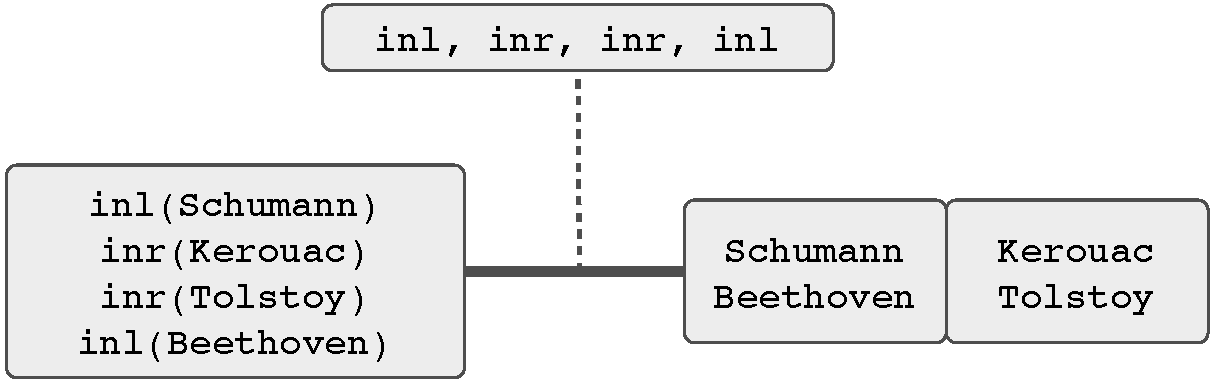
\includegraphics[width=75mm]{images/ex2-0.pdf} \\[.9ex]
        \parbox \lw{(a) the initial \replicas: a tagged list of composers and authors on
        the left; a pair of lists on the right; a complement storing just
        the tags}
        \\[3ex]
        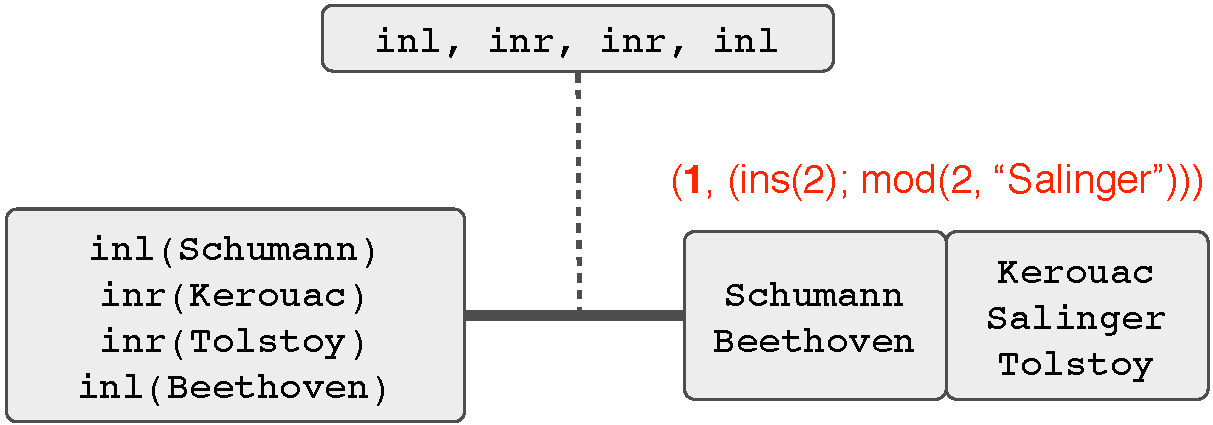
\includegraphics[width=75mm]{images/ex2-1.pdf} \\
        \parbox \lw{\begin{center}(b) an element is added to one of
            the partitions\end{center}} \\[2ex]
        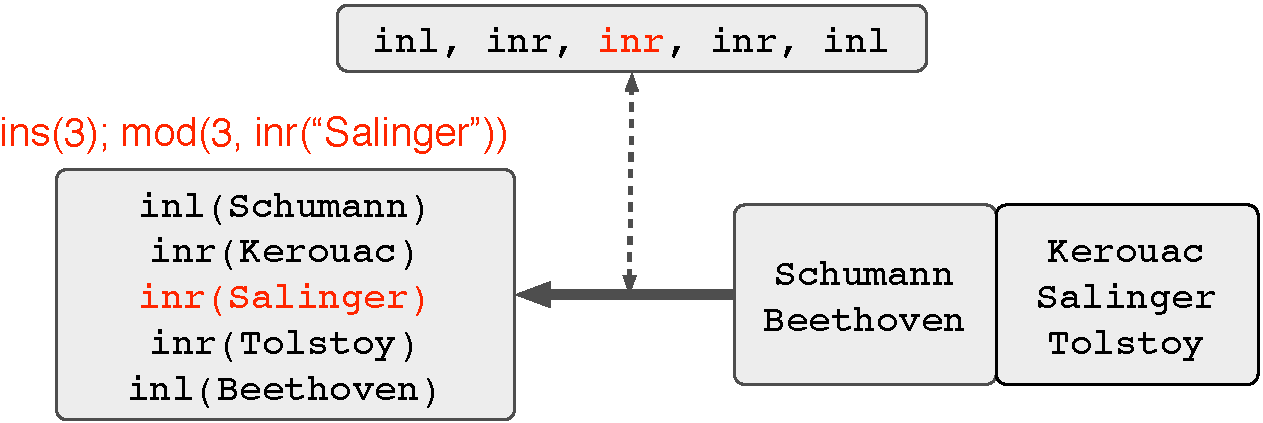
\includegraphics[width=75mm]{images/ex2-2.pdf} \\
        \parbox \lw{\begin{center}(c) the complement tells how to translate the
            index\end{center}} \\[.7ex]
    \end{tabular}
    \caption{A lens with complement.}
    \label{fig:example-partition}
\end{figure}

We sometimes need lenses to have a little more structure than this simple
example suggests. 
To see why, consider defining a {\em partitioning} lens $p$ between
the sets $\partial((X+Y)\LIST)$ and $\partial(X\LIST \times Y\LIST)$.
Figure~\ref{fig:example-partition} demonstrates the behavior of this lens.
%
In part (a), we show the original \replicas: on the left, a single list that
intermingles authors and composers (with {\sf inl/inr} tags showing which is
which), and on the right a pair of homogeneous (untagged) lists, one for
authors and one for composers. Now consider an edit, as in (b), that inserts
a new element somewhere in the author list on the right. It is clear that we
should transport this into an insertion on the left \replica, but where, exactly,
should we insert it?  If the $\dputl$ function is given just an
insertion edit for the homogeneous author list and nothing else, there is no
way it can translate this edit into a sensible position in the combined list
on the left, since it doesn't know how the lists of authors and composers
are interleaved on the left.  

\iflater\bcp{People were not clear on why the complement was needed.  Also, in this
  example, even with the complement, there is still some arbitrary choice in
  where an inserted element on the right appears in the list on the left.}\fi

The solution is to store a small list, called a {\em complement}, off to the
side, recording the \emph{tags} ($\ml{inl}$ or $\ml{inr}$) from the
original, intermingled list, and pass this list as an extra argument to
translation.  We then enrich the types of the edit translation functions to
accept a complement and return a new complement, so that
%
\iffull \[ \else $ \fi
p.\dputr \in \partial((X+Y)\LIST) \times C \to \partial(X\LIST \times Y\LIST)
\times C
\iffull \] \else $ \fi
and
\iffull \[ \else $ \fi
p.\dputl \in \partial(X\LIST \times Y\LIST) \times C \to \partial((X+Y)\LIST)
\times C
\iffull .\] \else $. \fi
Part (c)
demonstrates the use (and update) of the complement when translating the
insertion.

Note that the complement stores just the {\sf inl/inr} tags, not the actual
names of the authors and composers in the left-hand list.  \iflater\finish{This next
statement made people suspicious---we need to go into more detail.}\fi In general, the
information stored in $C$ will be much smaller than the
information in the \replicas; indeed, our earlier example illustrates the
common
case in which $C$ is the trivial single-element set $\Unit$.  The
translation functions manipulate just the complements and the edits, which
are also small compared to the size of the \replicas.

%% \finish{Someplace, we need to talk about what happens to edits that don't
%%   make sense on the current state.  There are three possibilities, with a
%%   tradeoff between size of representations and ``accuracy'' of edits:
%%   \begin{itemize}
%%   \item Embed a description of the exact state in the edit and say that the
%%   edit only applies to this state.  This is what Diskin, etc., do.  But it
%%   means that edits are very large.
%%   \item Allow any edit to apply to any state.  Then there are two
%%   sub-possibilities:
%%   \begin{itemize}
%%   \item keep it total but make it behave like the identity (or some other
%%   arbitrary choice) anywhere it doesn't ``make sense''
%%   \item make it partial
%%   \end{itemize}
%%   \end{itemize}
%% }
%% \finish{
%% Old text: Other authors model {\edit}s in other ways; for example, Stevens
%% \finish{citation} chooses functions whose domain and range are equal.
%% Functions are a nice model in some circumstances, but are difficult to
%% inspect: the only operation that can be performed is to apply them to some
%% concrete argument.  Monoids subsume these functions, and some instantiations
%% offer more reflective representations of edits.}

\sect{Edit Lenses}
\label{sec:semantics}

A key design decision in our formulation of edit lenses is to separate the
{\em description} of edits from the {\em action} of applying an edit to a
state.  This separation is captured by the standard mathematical notions of
{\em monoid} and {\em monoid action}.

\begin{defn}
%% \bcp{why do we say a triple here and in
%%     3.2.3, but other places just name the components (e.g., defn of
%%     category)?} 
A \emph{monoid} is a triple $\left<M,\cdot_M,\ONE_M\right>$ of a set
$M$, an associative binary operation $\cdot_M \in M \times M
\to M$, and a unit element $\ONE_M \in M$ --- that is, with $\cdot_M$ and $\ONE_M$ such that
\iffull
\begin{eqnarray*}
x\cdot_M(y\cdot_M z) = (x\cdot_M y) \cdot_M z\\
\ONE_M\cdot_M x = x = x \cdot_M \ONE_M .
\end{eqnarray*}
\else
$x\cdot_M(y\cdot_M z) = (x\cdot_M y) \cdot_M z $ and
$\ONE_M\cdot_M x = x = x \cdot_M \ONE_M$.
\fi
\end{defn}
When no confusion results, we use $M$ to denote both the set and the
monoid, drop subscripts from $\cdot$ and $\ONE$, and write $mn$ for
$m \cdot n$.  
%% In more standard terminology, a ``monoid'' in our sense would
%% be called a \emph{partial monoid}\iflater~\cite{partialmonoids}\fi, but
%% since we always work with partial monoids we find it convenient to drop the
%% qualifier.

The unit element represents a ``change nothing'' edit.  Multiplication of
edits corresponds to packaging up multiple edits into a single one
representing their combined effects\iffull{} (this might be useful, for example, for
offline editing)\fi.

Modeling edits as monoid elements gives us great flexibility in 
concrete representations.
%
The simplest edit language is a {free monoid} whose elements are just words
over some set of primitive edits and whose multiplication is
concatenation.  
%
However, it may be useful to put 
more structure on edits, either (a) to allow 
more compact representations or (b) to capture the intuition that edits to
different parts of a structure do not interfere with each other and can thus
be applied in any order.  We will see an example of (b) in 
\S \ref{sec:monoid-laws}. For a simple example of 
(a), recall from
\S \ref{sec:delta-examples} that, for every set $X$, we can form an {\em
  overwrite} monoid where the edits are just the elements of $X$ together
with a fresh unit element---i.e., edits can be represented as elements of
the disjoint union $\Unit + X$. Combining two edits in this monoid
simply drops the second (unless the first is the unit):
\iffull
\[
\mlinl{\unit} \cdot e = e \qquad
\mlinr{x} \cdot e = \mlinr x
\]
\else
$\mlinl{\unit} \cdot e = e$ and $\mlinr{x} \cdot e = \mlinr x$.
\fi
These equations allow this edit language to represent an arbitrarily long
sequence of updates using a single element of $X$ (and, {\em en passant}, to
recover state-based lenses as a special case of edit lenses). \iflater\bcp{Would it
  actually work to build a whole set of lens combinators with these edits?
  Or are we just saying that, for an arbitrary set $X$, there is an identity
  lens on this module over $X$?  What, exactly, are we saying?}\fi
%
The monoid framework can also accommodate more abstract notions of edit.  For
example, the set of all total \iffull(respectively, partial) \fi
functions from a set $X$ to itself forms a monoid, where the multiplication
operation is function composition\iffull\ (and the unit is the
identity function)\fi. This is essentially the form of edits considered by
Stevens~\cite{stevens2008tat}\iflater\finish{Not just Stevens---we should
  find a few more citations for this idea.}\fi.  \iflater\bcp{Same question for this one.  At a minimum, we should say that we are not dealing with these examples in detail in the rest of the paper.}\fi
%
We mostly focus on the simple case where edit languages are free monoids.
\S \ref{sec:monoid-laws} considers how additional laws can be added to the
product and sum lens constructions\iffull\ (laws for lists and general
containers are left for future work)\fi.

\iffull
\begin{defn}
    Given monoids $M$ and $N$, a \emph{monoid homomorphism} is a function $h
    \in M \to N$ that satisfies two laws:
    \begin{align*}
        h(\ONE_M) &= \ONE_N \\
        h(m \cdot_M m') &= h(m) \cdot_N h(m')
    \end{align*}
\end{defn}
Monoid homomorphisms are structure-preserving maps, and we will see many
specializations of this definition below. An example of a homomorphism in
the case where the two monoids $M$ and $N$ are both free monoids is any
operation that acts pointwise on the elements of the lists. Having defined
monoids, which model descriptions of edits, we will now model the operation
that performs an edit on a particular object.

\begin{defn}
    Given a  monoid $M$ and a set $X$, a \emph{monoid action} of $M$ on $X$
    is a monoid homomorphism from $M$ to the monoid of partial functions $X
    \partialto X$. Unrolling this definition, this means an action is a
    partial function $\odot \in M \to (X \partialto X)$, or equivalently,
    $\odot \in M \times X \partialto X$, satisfying two laws:
    \begin{align*}
        \ONE \odot x &= x \\
        (m \cdot n) \odot x &= m \odot (n \odot x)
    \end{align*}
\end{defn}
We use $X \partialto Y$ for the space of partial functions with domain $X$
and codomain $Y$. If $f \in X \partialto Y$, we will write $f(x)\Defined$ to
mean that $f$ is defined at $x$.
\else

\begin{defn}
    Given a  monoid $M$ and a set $X$, a \emph{monoid action} on $M$ and $X$
    is a partial function $\odot \in M \times X \partialto X$ satisfying two laws:
    $\ONE \odot x = x$ and $(m \cdot n) \odot x = m \odot (n \odot x)$.
\end{defn}
\fi%full
%
As with monoid multiplication, we often elide the monoid action symbol,
writing $mx$ for $m \odot x$.  In standard mathematical terminology, a
monoid action in our sense might instead be called a ``partial monoid
action\commaquote but since we always work with partial actions we find it
convenient to drop the qualifier.

A bit of discussion of partiality is in order.  
Multiplication of edits is a total operation: given two descriptions of
edits, we can always find a description of the composite actions of doing
both in sequence.  On the other hand, {\em applying} an edit to a particular
state may sometimes fail.
%
This means we need to work with expressions and equations involving
partial operations. As usual, any term that contains an undefined
application of an operation to operands is undefined---there is no way of
``catching'' undefinedness. An equation between possibly undefined terms 
(e.g., as in the definition above) 
means that if either side is defined then so is the other, and their values
are equal (Kleene equality).

Why deal with failure explicitly, rather than keeping edit application total
and simply defining our monoid actions so that applying an edit in a state
where it is not appropriate yields the same state again (or perhaps some
other state)?  One reason is that it seems natural to directly address the
fact that some edits are not applicable in some states, and to have a
canonical outcome in all such cases.  A more technical reason is that, when
we work with monoids with nontrivial equations, making inapplicable edits
behave like the identity is actually
wrong.%
%
\footnote{Here is a slightly contrived example.  Suppose that the set of
  states is natural numbers and that edits have the form $(x\mapsto y)$,
  where the intended interpretation is that, if the current state is $x$,
  then the edit yields state $y$.  It is reasonable to impose the equation
  $(y\mapsto z)\cdot(x\mapsto y) = (x\mapsto z)$, allowing us to represent
  sequences of edits in a compact form.  But now consider what happens when
  we apply the edit $(5\mapsto 7)\cdot(3\mapsto 5)$ to the state $5$.  The
  second monoid action law demands that $((5\mapsto 7)\cdot(3\mapsto 5))
  \odot 5 = (5\mapsto 7)\odot((3\mapsto 5) \odot 5)$, which, by the equation
  we imposed, is the same as $(3\mapsto 7) \odot 5 = (5\mapsto
  7)\odot((3\mapsto 5) \odot 5)$.  But the left-hand side is equal to $5$
  (since the edit $(3\mapsto 7)$ does not apply to the state $5$), while the
  right-hand side is equal to $7$ (since the first edit, $(3\mapsto 5)$, is
  inapplicable to the state $5$, so it behaves like the identity and returns
  $5$ from which $(5\mapsto 7)$ takes us to $7$), so the action law is
  violated.}

However, although the framework allows for the possibility of edits failing,
we still want to know that the edits produced by our lenses will never
actually fail when applied to \replica states arising in practice.  This
requirement, corresponding to the {\em totality} property of previous
presentations of lenses~\cite{Focal2005}, is formalized in Theorem
\ref{nofail}.  In general, we adopt the design principle that partiality
should be kept to a minimum; this simplifies the definitions.

%% Notice that the second law implies that if $m\odot(n\odot x)$ is
%% defined then $m\cdot n$ must be defined and conversely, if $n\odot x$
%% is undefined then $(m\cdot n)\odot x$ must also be undefined for all
%% $m$ even if $m\cdot n$ is defined.

\iflater
\finish{A monoid action is a monoid homomorphism from $M$ to $X \to X$. Can
tie this back to the Stevens work, too, maybe?}
\fi

It is convenient to bundle a particular choice of monoid and monoid
action, plus an initial element, into a single structure:

\begin{defn}
    A \emph{module} is a tuple $\left<X,\, \init_X,\, \partial
    X,\,\odot_X\right>$ comprising a set $X$, an element $\init_X\in X$, a monoid 
    $\partial X$, and a monoid action $\odot_X$ of $\partial X$ on $X$.
\end{defn}
If $X$ is a module, we refer to its first component by either
$|X|$ or just $X$, and to its last component by $\odot$ or simple
juxtaposition.

We will use modules to represent the structures connected by lenses.  Before
coming to the definition of lenses, however, we need one last ingredient:
the notion of a {\em stateful homomorphism} between monoids.  As we saw in
\S \ref{sec:delta-examples}, there are situations where the information in an
edit may be insufficient to determine how it should be translated---we may
need to know something more about how the two structures correspond. The
exact nature of the extra information needed varies according to the lens.
%
To give lenses a place to store such auxiliary information, we
follow\symmlenses and allow the edit-transforming
components of a lens (the $\dputr$ and $\dputl$ functions) to take a {\em
  complement} as an extra input and return an updated complement as an extra
output.
%
\iflater
\discuss{Not sure there's time to change it now, but I found while writing
  that explanation that the word ``complement'' was quite awkward---I kept
  wanting to say just ``state.''  Moreover, the term is technically a bit
  tenuous now, since what we store is not, in fact, anything like a
  complement in the old database sense.}  \soon{complement becomes correspondence}
\fi

\iffull
\begin{defn}
    Given a monoid $M$ and a {\em complement set} $C$, one can define the
    \emph{stateful monoid} $\mathit{State}_C(M)$ whose elements are
    functions $C \to M \times C$. The unit and multiplication are given by
    \begin{align*}
        \ONE(c) ={}& (\ONE,c) \\
        (m \cdot n)(c) ={}& \mllet (m',c') = m(c) \\
        & \phantom{\mllet} (n',c'') = n(c') \\
        & \mlinb (m' \cdot n',c'')
    \end{align*}
\end{defn}
Functional programmers will recognize this monoid's multiplication as a
lifting of the underlying monoid's multiplication into the state monad (and
likewise the unit is a lifting of the underlying unit).

\begin{defn}
    Given monoids $M$ and $N$ and a complement set $C$, a \emph{stateful
    monoid homomorphism} from $M$ to $N$ over $C$ is a monoid
    homomorphism $h \in M \to \mathit{State}_C(N)$. In the following, we
    will typically treat $h$ as if it were a two-argument function; so,
    unrolling the definition of homomorphism, $h$ satisfies two laws:
    \infax{h(\ONE_M,c) = (\ONE_N,c)}
    \infrule{h(m,c) = (n,c') \andalso h(m',c') = (n',c'')}
            {h(m' \cdot m,c) = (n' \cdot n,c'')}
\end{defn}
\else
\begin{defn}
Given monoids $M$ and $N$ and a {\em complement set} $C$, a \emph{stateful monoid
  homomorphism} from $M$ to $N$ over $C$ is a function $h \in M \times C \to
N \times C$ satisfying two laws:
%
\vspace*{-1ex}
\infrule{}{h(\ONE_M,c) = (\ONE_N,c)}
\infrule{
         h(m,c) = (n,c') \andalso h(m',c') = (n',c'')
}{
         h(m' \cdot_M m,c) = (n' \cdot_N n,c'')
}
%
These are basically just the standard monoid homomorphism laws, except that
$h$ is given access to some internal state $c \in C$ that it uses (and
updates) when mapping from $M$ to $N$; in the second law, we must thread the
state $c'$ produced by the first $h$ into the second use of $h$, and we
demand that both the result and the effect on the state should be the same
whether we send a composite element $m' \cdot m$ through $h$ all at once or
in two pieces.
\end{defn}
\fi

The intended usage of an edit lens is as follows. There are two users,
one holding an element of $X$ the other one an element of $Y$\ifdelta, both
referred to hereafter as {\em \replicas}\fi. Initially, they hold $\init_X$ and
$\init_Y$, respectively, and the lens is initialized with complement
$\ell.\missing$. The users then perform actions and propagate them across
the lens. An action consists of producing an edit $\dx$ (or $\dy$), applying
it to one's current \replica $x$ (resp.\ $y$), putting the edit through the lens
to obtain an edit $\dy$ (resp.\ $\dx$), and asking the user on the other
side to apply $\dy$ ($\dx$) to their \replica.  In the process, the internal
state $c$ of the lens is updated to reflect the new correspondence between
the two \replicas.
\iffull

\fi%
We further assume there is some {\em consistency} relation $K$ between $X$,
$Y$, and $C$, which describes the ``synchronized states'' of the \replicas
and complement.  This gives us a natural way to state the totality
requirement discussed above: if we start in a consistent state, make a
successful edit (one that does not fail at the initiating side), and put it
through the lens, the resulting edit is guaranteed (a) to be applicable on
the receiving side and (b) to lead again to a consistent state.  We make no
guarantees about edits that fail at the initiating side: these should not be
put through the lens.

\begin{defn}\label{defn:lens}
A \emph{symmetric edit lens} between modules $X$ and $Y$ consists of a
complement set $C$, a distinguished element $\missing\in C$, 
two stateful monoid homomorphisms 
\iffull
\[
\begin{array}{lcl}
\dputr &\in& \partial X \times C \to \partial Y \times C \\
\dputl &\in& \partial Y \times C \to \partial X \times C
\end{array}
\]
\else
$\dputr \in \partial X \times C \to \partial Y \times C$ and
$\dputl \in \partial Y \times C \to \partial X \times C$, 
\fi
%
%% total functions 
%% \[
%% \begin{array}{lcl}
%% \dputr &\in& \partial X \times C \to \partial Y \times C \\
%% \dputl &\in& \partial Y \times C \to \partial X \times C
%% \end{array}
%% \]
%% such that \infax{\dputr(\ONE,c)=(\ONE,c) \qquad \dputl(\ONE,c)=(\ONE,c)}
%% \infrule{ \dputr(\dx_2,c)=(\dy_2,c') \quad
%%   \dputr(\dx_1,c')=(\dy_1,c'') }{ \dputr(\dx_1\ \dx_2,c)=(\dy_1\
%%   \dy_2, c'') } \infrule{ \dputl(\dy_2,c)=(\dx_2,c') \quad
%%   \dputl(\dy_1,c')=(\dx_1,c'') }{ \dputl(\dy_1\ \dy_2,c)=(\dx_1\
%%   \dx_2, c'') } 
and a ternary {\em consistency relation}
$K\subseteq |X|\times C\times |Y|$ such that
\begin{itemize}
\item $(\init_X,\missing,\init_Y)\in K$;
\item if $(x,c,y)\in K$ and $\dx\ x$ is defined and $\dputr(\dx,c)=(\dy,c')$, then $\dy\ y$ is also defined and $(\dx\ x,c',\dy\ y)\in K$;
\item if $(x,c,y)\in K$ and $\dy\ y$ is defined and $\dputl(\dy,c)=(\dx,c')$, then $\dx\ x$ is also defined and $(\dx\ x,c',\dy\ y)\in K$.%
%
\iffull
\footnote{One might consider a more general format with ``creation''
  operations $\creater\in X\rightarrow Y\times C$ and symmetrically
  $\createl$.  This format actually arises as a special case of the one
  above by choosing the edit monoids to include operations of the form
  $\text{set}(x)$ for $x\in X$, with action $\text{set}(x)\odot x'=x$. One
  can then define $\creater(x,c) = \dputr(\text{set}(x),c)$.}
\fi
%
\end{itemize}
% \discuss{BCP will add a note about binary consistency relations.  Dual role: Important sanity check on dputs, but also a part of the external specification of the lens.}
\end{defn}
Since symmetric edit lenses are the main topic of this \ifdissertation
chapter\else paper\fi, we will
generally write ``edit lens'' or just ``lens'' for these,
deploying additional adjectives to talk about other variants such
as \iflater\finish{the asymmetric variant or} \fi the state-based
symmetric lenses of\symmlenses.\ifdissertation\ Similarly, we will co-opt
the notation of the previous chapter, reusing many component names, $\lens$
for the type of edit lenses, $\equiv$ for lens equivalence, and so on. When
it is important to differentiate, we will use a subscript $s$ for
state-based concepts, as in $\sslens$ or $\equiv_s$.\fi

The intuition about $K$'s role in guaranteeing totality can be formalized as
follows.

\begin{defn}
Let $\ell \in X\lens Y$ be a lens. A \emph{dialogue} is a sequence of
edits---a word in $(\partial X+\partial Y)\LIST$. The {partial}
function
\iffull\[\else $ \fi
\ell.\run \in (\partial X+\partial Y)\LIST\partialto   X\times   \ell.C\times Y
\iffull\]\else $ \fi
is defined by:
\infrule{}{\ell.\run(\NIL) = (\init_X,\ell.\missing,\init_Y)}
\infrule{
    \ell.\run(w)=(x_0,c,y_0)
    \andalso  
    \ell.\dputr(\dx_1,c)=(\dy_1,c_1)
  }{
    \ell.\run(\mlinl{\dx_1} \CONS w) = (\dx_1\,x_0,c_1,\dy_1\,y_0)
  }
\infrule{
    \ell.\run(w)=(x_0,c,y_0)
    \andalso  
    \ell.\dputl(\dy_1,c)=(\dx_1,c_1)
  }{
    \ell.\run(\mlinr{\dy_1} \CONS w) = (\dx_1\,x_0,c_1,\dy_1\,y_0)
  }
\end{defn}

\begin{theorem}\label{nofail}
Let $w$ be a dialogue and suppose that $\ell.\run(w)=(x,c,y)$---in
particular, all the edits in $w$ succeed.
Let $\dx\in\partial X$ be an edit with $\dx\ x$ defined. If
$(\dy,c')=\ell.\dputr(\dx,c)$ then $\dy\ y$ is also defined. An analogous
statement holds for $\dputl$.
\end{theorem}

\iffull
\begin{proof}
By induction on $w$ we can easily show that $(x,c,y)\in \ell.K$. The claim
then follows from the axioms for lenses.
\end{proof}
\fi

\iflater \finish{We need some discussion of why these laws are the
  right ones.  One justification is that they are essentially just
  (stateful versions of) the monoid homomorphism laws.  Another is
  that they give rise to a nice correspondence with state-based lenses
  (is that true?).}  \fi

Beyond its role in guaranteeing totality, the consistency relation in a lens
plays two important roles.  First, it is a sanity check on the behavior of
$\dputr$ and $\dputl$.  Second, if we project away the middle component, we
can present it to programmers as documentation of the synchronized states of
the two \replicas---i.e., as a partial {\em specification} of $\dputr$ and
$\dputl$.

One technical issue arising from the definition of edit lenses is that the
hidden complements cause many important laws---like associativity of
composition---to hold only up to {\em behavioral equivalence}.  This phenomenon
was also observed in \ifdissertation\S\ref{equiv}\else\cite[\S
3]{HofmannPierceWagner10}\fi\ for the case of
symmetric state-based lenses, and the appropriate behavioral equivalence
for edit lenses is a natural refinement of the one used there (taking the
consistency relations into account).

\begin{defn}[Lens equivalence]
Two lenses $k,\ell:X\lens Y$ are {\em equivalent} (written $k \equiv \ell$) if,
for all dialogues $w$, 
\begin{itemize}
\item $k.\run(w)$ is defined iff $\ell.\run(w)$ is defined;
\item if $k.\run(w)=(x,c,y)$ and $\ell.\run(w)=(x',d,y')$, then $x=x'$ and
$y=y'$; and
\item if  $k.\run(w)=(x,c,y)$ and $\ell.\run(w)=(x',d,y')$ and $\dx\ x$ is defined and $\ell.\dputr(\dx,c)=(\dy,\_)$ and 
 $k.\dputr(\dx,d)=(\dy',\_)$ then $\dy=\dy'$, and the analogous property for $\dputl$. 
\end{itemize} 
\end{defn}
(Note that the second clause is actually implied by the third.)
% We write $X \Lens Y$ for the set of equivalence classes of lenses
% from $X$ to $Y$.  When $\ell$ is a lens, we write $\EQCLASS{\ell}$
% for the equivalence class of $\ell$ (that is, $\ell \in X\lens Y$
% iff $\EQCLASS{\ell} \in X\Lens Y$).  Where no confusion results, we
% abuse notation and drop these brackets, using $\ell$ for both a lens
% and its equivalence class.  \finish{Do we actually need this
%   convention now?  Doesn't seem like we're making much use of
%   equivalence classes in this paper.}
% \end{defn}

Since the complements of the two lenses in question may not even have
the same type, it does not make sense to require that they be
equal. Instead, the equivalence hides the complements, relying on the
observable effects of the lens actions. However, by finding a
relationship between the complements, we can prove lens
equivalence with a bisimulation-style proof principle:
\begin{theorem}\label{thm:bisim}
Lenses $k,\ell:X\lens Y$ are equivalent iff there exists a relation
$S\subseteq X\times k.C\times \ell.C\times Y$ such that  
\iffull \begin{itemize} \fi
\iffull \item \else (1) \fi $(\init_X,k.\missing,\ell.\missing,\init_Y)\in S$;
\iffull \item \else (2) \fi if $(x,c,d,y)\in S$ and $\dx\ x$ is defined, then if $(\dy_1,c')=
k.\dputr(\dx,c)$ and $(\dy_2,d')=
\ell.\dputr(\dx,d)$, then $\dy_1=\dy_2$ and $(\dx\ x,c',d',\dy_1\ y)\in
S$; and
\iffull \item \else (3) \fi analogously for $\dputl$. 
\iffull \end{itemize} \fi
\end{theorem}

\iffull
\begin{pf}
  For the ``if'' direction we prove by induction on dialogues that if
  $k.\run(w)$ is defined then so is $\ell.\run(w)$ and vice versa and
  if $k.\run(w)=(x,c,y)$ and $\ell.\run(w)=(x',d,y')$ then $x=x'$ and
  $y=y'$ and $(x,c,d,y)\in S$. For the converse we define
  $(x,c,d,y)\in S$ iff there exists a dialogue $w$ such that
  $k.\run(w)=(x,c,y)$ and $\ell.\run(w)=(x,d,y)$ 
% \finish{Checked that
%     this proof is good for the new notion of equivalence. }
\end{pf}

\begin{theorem}
    Lens equivalence is an equivalence relation.
\end{theorem}
\begin{pf}
    Reflexivity: the set $\{(x,c,c,y) \mid (x,c,y) \in \ell.K\}$ witnesses the
    equivalence $\ell\equiv\ell$ for any $\ell$.

    Symmetry: if the set $S$ witnesses the equivalence $k\equiv\ell$, then
    the set $\{(x,d,c,y) \mid (x,c,d,y) \in S\}$ witnesses the equivalence
    $\ell \equiv k$.

    Transitivity: if $S$ witnesses $j \equiv k$ and $T$ witnesses
    $k\equiv\ell$, then
    \[\{(x,c,e,y) \mid \exists d. (x,c,d,y) \in S \land (x,d,e,y) \in T\}\]
    witnesses $j\equiv\ell$. The verification is straightforward.
\end{pf}
\fi

\iffull
\iflater
\discuss{Not sure exactly where this lemma belongs.  When is it used?}The
following lemma asserts that dialogues and runs make sense on the level of
equivalence classes. The proof is a direct induction on runs.
\begin{lemma}
Let $k,\ell \in X\lens Y$ be equivalent lenses ($k\equiv \ell$). Let $w$
be a dialogue and $k.\run(w)=(x,c,y)$ and
$\ell.\run(w)=(x',c',y')$. Then $x=x'$ and $y=y'$. 
\end{lemma}

\discuss{I find this next observation about not being visible at the level
  of equivalence classes to be more confusing than enlightening.  Could we
  just drop it?}
\discuss{Re-reading it, I tend to agree. Probably, we should rather dwell on 
the ``projecting out the complement'' point of view. --Martin}
The consistency relations $K$ are not visible at the level
of equivalence classes of lenses not least because they involve the
complement. As we have seen, their mere presence guarantees that reasonable
edits succeed and this phenomenon is observable at the level of equivalence
classes. But consistency relations are also useful to assert certain shared
properties between the states that are ``synchronized'' by the lens. We now
give a complement-free version of this:

\begin{defn}
A lens $\ell \in X\lens Y$ {\em maintains} a relation $R\subseteq X\times Y$ if,
for any dialogue $w$ and $\ell.\run(w)=(x,c,y)$, we have $x\mathrel{R}y$. 
\end{defn}

\begin{theorem}
If $k\equiv\ell$ are equivalent lenses between $X$ and $Y$, then $k$
maintains a relation $R$ iff $\ell$ does.
%
Moreover, $\ell$ preserves $R$ iff there exists a relation $S\subseteq
X\times\ell.C\times Y$ such that 
\begin{itemize}
\item $(\init_X,\ell.\missing,\init_Y)\in S$;
\item whenever $(x,c,y)\in S$ and
$\dx\ x$ is defined, $\dy\ y$ is also defined and $(\dx\ x,c',\dy\
y)\in S$ when $(\dy,c')=\dputr(\dx,c)$; 
\item the analogous condition for $\dputl$; and
\item $(x,c,y)\in S$ implies $(x,y)\in R$.
\end{itemize}
\end{theorem}

\iffull
\begin{pf}
The ``if'' direction is an easy induction on dialogues. For the ``only
if'' direction we use the relation $S=\{(x,c,y)\mid xRy\wedge \exists
w.\ell.\run(w)=(x,c,y)\}$. 
\finish{Needs to be updated for the new defn of equivalence.}
\end{pf}
\fi
\fi
\fi

\sect{Edit Lens Combinators}\label{sec:combinators}

\iflater\discuss{We don't actually formalize the ``overwrite edits'' lens
  constructor (which takes a set to a module).  We should, since we use it
  in Section 2!}\fi

\iflater
\finish{The extra (fibrationish) laws need to be checked for everything
  here.}\bcp{I guess we've dropped these laws now, but it would be nice to
  get back to discussing them someplace.}
\fi

We have proposed a semantic space of edit lenses and justified its design.
But the proof of the pudding is in the syntax---in whether we can actually
build primitive lenses and lens combinators that live in this semantic space
and that do useful things.

\paragraph*{Generic Constructions}

As a first baby step, here is an identity lens that connects identical
structures and maps edits by passing them through unchanged.

\iffull \begin{defn}[Identity]\  \fi
        \lensdef{w_id}
        {\id_X \in X \lens X}
        {
            C &=& \Unit \\
            K &=& \{ (x,\unit,x) \;|\; x \in X \} \\
            \dputr(\dx,\unit) &=& (\dx,\unit) \\
            \dputl(\dx,\unit) &=& (\dx,\unit)
}
%
Here and below, we elide the definition of the $\missing$ component when
$C=\Unit=\{\unit\}$, since it can only be one thing.

\iffull
\begin{lemma}\ 
    $\id.\dputr$ and $\id.\dputl$ are stateful homomorphisms, and the
    relation $\id.K$ is preserved.
    \label{id-goodlens}
\end{lemma}
\begin{proof}
    Showing that $\dputr$ is a homomorphism involves showing that
    $\id.\dputr(\ONE,\unit)=(\ONE,\unit)$, which is direct, and that if
    $\id.\dputr(\dx,c)=(\dy,c')$ and $\id.\dputr(\dx',c')=(\dy',c'')$,
    then $\id.\dputr(\dx'\dx,c)=(\dy'\dy,c'')$. Since $c=c'=c''=\unit$, it
    follows directly that $\dy=\dx$ and $\dy'=\dx'$, so the final claim is
    true. A similar argument shows that $\dputl$ is a homomorphism.

    To show that $K$ is preserved, choose a consistent triple
    $(x,\unit,x)$ and observe that $\dputr(\dx,\unit)=(\dx,\unit)$ results
    in another consistent triple $(\dx\;x,\unit,\dx\;x)$. A similar argument
    for $\dputl$ applies.
\end{proof}
\else
In lens definitions like this one, the upper box serves both as a typing
rule and as the implicit statement of a theorem saying that the functions in
the box below it inhabit the appropriate types and satisfy the corresponding lens
laws. For lens combinators, the definition also makes an implicit statement
about compatibility with lens equivalence. For brevity, and because they are
generally straightforward, we usually elide these theorems.
\fi
\iffull \end{defn} \fi

Now for a more interesting case:  Given lenses $k$ and $\ell$ connecting $X$ to
$Y$ and $Y$ to $Z$, we can build a composite lens $k;\ell$ that connects $X$
directly to $Z$.  Note how the complement of the composite lens includes
a complement from each of the components, and how these complements
are threaded through the $\dputr$ and $\dputl$ operations.
\iffull \begin{defn}[Composition]\  \fi
        \lensdef{w_composition}
        {\infruleplain{k \in X \lens Y \qquad \ell \in Y \lens Z}{k;\ell \in X \lens Z}}
        {
            C &=& k.C \times \ell.C \\
            \missing &=& (k.\missing , \ell.\missing) \\
            K &=& \{ (x,(c_k,c_\ell),z) \;|\; \\
                        && \qquad \exists y. \;
                        (x,c_k,y) \in k.K  \\
                        && \qquad\hspace{1em} \wedge 
                        (y,c_\ell,z) \in \ell.K\ 
                  \} \\
            \dputr(\dx, (c_k, c_\ell))
            &=& \mllet (\dy, c_k') = k.\dputr(\dx, c_k) \mline \\
            & & \mllet (\dz, c_\ell') = \ell.\dputr(\dy, c_\ell) \mline \\
            & & (\dz, (c_k', c_\ell')) \\
            \dputl(\dz, (c_k, c_\ell))
            &=& \mllet (\dy, c_\ell') = \ell.\dputl(\dz, c_\ell) \mline \\
            & & \mllet (\dx, c_k') = k.\dputl(\dy, c_k) \mline \\
            & & (\dx, (c_k', c_\ell'))
        }
\iffull \end{defn} \fi

\iffull
\begin{lemma}
    Given that $k$ and $\ell$ are lenses, this construction defines a lens:
    \begin{itemize}
        \item $\dputr$ and $\dputl$ are stateful monoid homomorphisms,
        \item relation $K$ is preserved, and
        \item it respects lens equivalence: if $k \equiv k'$ and
            $\ell\equiv\ell'$, then $k;\ell \equiv k';\ell'$.
    \end{itemize}
    \label{composition-goodlens}
\end{lemma}
\begin{pf}\ 

  $\dputr$ is a stateful monoid homomorphism. Since $k.\dputr$ and
  $\ell.\dputr$ are homomorphisms, we know that
  \begin{align*}
      k.\dputr(\ONE,c_k) &= (\ONE,c_k) \\
      \ell.\dputr(\ONE,c_\ell) &= (\ONE,c_\ell)
  \end{align*}
  and hence that
  \[\dputr(\ONE,(c_k,c_\ell))=(\ONE,(c_k,c_\ell)).\]
  Choosing arbitrary $\dx,\dx',c_k,c_\ell$, we can define
  \begin{align*}
      (\dy,c_k') &= k.\dputr(\dx,c_k) \\
      (\dy',c_k'') &= k.\dputr(\dx',c_k') \\
      (\dz,c_\ell') &= \ell.\dputr(\dy,c_\ell) \\
      (\dz',c_\ell'') &= \ell.\dputr(\dy',c_\ell')
  \end{align*}
  and observe that since $k.\dputr$ and $\ell.\dputr$ are homomorphisms, we
  then know:
  \begin{align*}
      k.\dputr(\dx'\dx,c_k) &= (\dy'\dy,c_k'') \\
      \ell.\dputr(\dy'\dy,c_\ell) &= (\dz'\dz,c_\ell'')
  \end{align*}
  We can now calculate
  \begin{align*}
      (k;\ell).\dputr(\dx,(c_k,c_\ell)) &= (\dz,(c_k',c_\ell')) \\
      (k;\ell).\dputr(\dx',(c_k',c_\ell')) &= (\dz',(c_k'',c_\ell'')) \\
      (k;\ell).\dputr(\dx'\dx,(c_k,c_\ell)) &= (\dz'\dz,(c_k'',c_\ell''))
  \end{align*}
  as necessary.

  $\dputl$ is a stateful monoid homomorphism. The argument is very similar
  to the above.

  The relation $K$ is respected. The triple
  $(\init_X,(k.\missing,\ell.\missing),\init_Z)$ is in $K$ because we can
  choose $y=\init_Y$ and observe that $(\init_X,k.\missing,\init_Y)\in k.K$
  and $(\init_Y,\ell.\missing,\init_Z)\in\ell.K$.

  Next, consider consistent triple $(x,(c_k,c_\ell),z)$ and some particular
  $y$ for which $(x,c_k,y) \in k.K$ and $(y,c_\ell,z)\in\ell.K$. (Such a $y$
  is guaranteed to exist by the definition of $K$.) Take $\dx$ for which
  $\dx\;x$ is defined and define:
  \begin{align*}
      (\dy,c_k') &= k.\dputr(\dx,c_k) \\
      (\dz,c_\ell') &= \ell.\dputr(\dy,c_\ell)
  \end{align*}
  By consistency of $k$, we know $\dy\;y$ is defined, and hence by
  consistency of $\ell$ we also know $\dz\;z$ is defined. Furthermore,
  $(\dx\;x,c_k,\dy\;y) \in k.K$ and $(\dy\;y,c_\ell,\dz\;z) \in \ell.K$, and
  hence $\dy\;y$ is a witness to the fact that $(\dx\;x,(c_k,c_\ell),\dz\;z)
  \in (k;\ell).K$, as needed. A similar argument shows that $\dputl$
  respects the consistency relation.

  The combinator respects lens equivalence.
  Suppose for simplicity that $k$ and $k'$ are identical (the general case then follows by symmetry and transitivity of $\equiv$). Using Theorem~\ref{eqchar} assume furthermore that $\ell\equiv \ell': X\lens Y$ 
by virtue of relation $S\subseteq X\times
  C\times C'\times Y$ assuming that $C$ and $C'$ are the complements of
  $\ell,\ell'$. We note $D$ the complement of $k\in Y\lens Z$. 

  Define simulation relation $T\subseteq X\times (C\times D)\times (C'\times D)\times Z$ by
\[
T = \{(x,(c,d),(c',d),z)\mid \exists y. (x,c,c',y)\in S \wedge (y,d,z)\in k.K\}
\]
Suppose that $(x,c,c',y)\in S$ and $(y,d,z)\in k.K$ thus $(x,(c,d),(c',d),z)\in T$ and 
$\dx\in \partial X$ such that $\dx\ x$ is defined. 
Let $(\dy,c_1)=\ell.\dputr(\dx,c)$ and $(\dy',c_1')=\ell'.\dputr(\dx,c')$ and further 
$(\dz,d_1)=k.\dputr(\dy,d)$ and  $(\dz',d_1')=k.\dputr(\dy',d)$. 

We should prove $\dz=\dz'$ and $d_1=d_1'$ and $(\dx\
x,(c_1,d_1),(c_1',d_1),\dz\ z)\in T$.  From $(x,c,c',y)\in S$ we get
$\dy=\dy'$ and $(\dx\ x,c_1,c_1',\dy\ y)\in S$ and $\dz=\dz'$ and
$d_1=d_1'$.  From $(y,d,z)\in k.K$ we then get $(\dy\ y,d_1,\dz\ z)\in
k.K$ and thus all that is required. 
\end{pf}
The following theorem establishes the properties necessary to show that
there is a category with modules as objects and equivalence classes of
lenses as arrows.  In what follows,
we will sometimes note how the properties of our lens
constructions can be restated in terms of standard categorical jargon, but
these observations are intended just as sanity checks; nothing depends on
them, and they can safely be ignored.
\begin{theorem}\ 
    \begin{itemize}
        \item $\id_X;\ell \equiv \ell;\id_Y \equiv \ell$
        \item $(k;\ell);m \equiv k;(\ell;m)$
    \end{itemize}
\end{theorem}
\begin{pf}
    The two relations given below witness $\id_X;\ell \equiv \ell$ and
    $\ell;\id_Y \equiv \ell$ respectively.
    \[\{(x,(c,\unit),c,y) \mid (x,c,y) \in \ell.K\}\]
    \[\{(x,c,(c,\unit),y) \mid (x,c,y) \in \ell.K\}\]

    The relation that re-associates the complements is a witness that
    $(k;\ell);m \equiv k;(\ell;m)$:
    \begin{align*}
        R ={}& \{(w,((c_k,c_\ell),c_m),(c_k,(c_\ell,c_m)),z) \\
            & \quad\mid c_k \in k.C, c_\ell \in \ell.C, c_m \in m.C\}
    \end{align*}
    Suppose we have an element of this relation and an edit $\dw$ for which
    $\dw \; w$ is defined; then define:
    \begin{align*}
        (\dx, c_k') &= k.\dputr(\dw, c_k) \\
        (\dy, c_\ell') &= \ell.\dputr(\dx, c_\ell) \\
        (\dz, c_m') &= m.\dputr(\dy, c_m)
    \end{align*}
    We can compute that:
    \begin{align*}
        ((k;\ell);m).\dputr(\dw,((c_k,c_\ell),c_m)) &= (\dz, ((c_k',c_\ell'),c_m')) \\
        (k;(\ell;m)).\dputr(\dw,(c_k,(c_\ell,c_m))) &= (\dz, (c_k',(c_\ell',c_m')))
    \end{align*}
    Thus, the two lenses output the same edit $\dz$ and transition to
    related complements, as required.
\end{pf}
\else
As might be expected, composition of lenses is associative, and
the identity lens is a unit for composition.  However, as mentioned above,
we need to be a 
little careful: it is not quite the case that $(k;\ell);m = k;(\ell;m)$---in
particular they have different complements.  Instead, what we can show is
that $(k;\ell);m \equiv k;(\ell;m)$\iffull---i.e., they behave the same, even if
they do not work quite the same internally\fi.  
\fi

Another simple lens combinator is dualization: for each lens $\ell \in X
\lens Y$, we can construct its dual, $\ell\op \in Y \lens X$, by swapping
$\dputr$ and $\dputl$.

\iffull
\begin{defn}[Dual]\ 
        \lensdef{w_dual}
        {\infruleplain{\ell \in X \lens Y}{\ell\op \in Y \lens X}}
        {
            C &=& \ell.C \\
            \missing &=& \ell.\missing \\
            K &=& \{ (y, c, x) \mid (x,c,y) \in \ell.K \} \\
            \dputr(\dy, c) &=& \ell.\dputl(\dy, c) \\
            \dputl(\dx, c) &=& \ell.\dputr(\dx, c)
        }
\end{defn}

\begin{lemma}
    Given that $\ell$ is a lens, $\ell\op$ is a lens: $\dputr$ and $\dputl$
    are stateful monoid homomorphisms, the consistency relation is
    preserved, and if $k\equiv\ell$ then $k\op\equiv\ell\op$.
    \label{op-goodlens}
\end{lemma}
\begin{proof}
    $\dputr$ and $\dputl$ are homomorphisms because $\ell.\dputl$ and
    $\ell.\dputr$ are, respectively. The preservation of $K$ is a direct
    consequence of $\ell$ preserving $\ell.K$. If $S$ is a bisimulation
    relation witnessing $k\equiv\ell$, then
    $S\op = \{(y,c,d,x) \mid (x,c,d,y) \in S\}$
    is a bisimulation relation witnessing $k\op\equiv\ell\op$.
\end{proof}

The name ${}\op$ is justified by the following theorem, which establishes
that $(-)\op$ is an involutive contravariant functor and hence that the
category of lenses is self-dual.

\begin{theorem}\ 
    \begin{itemize}
        \item $(\ell\op)\op\equiv\ell$
        \item $\id_X\equiv\id_X\op$
        \item $k\op;\ell\op \equiv (\ell;k)\op$
    \end{itemize}
\end{theorem}
\begin{proof}
    In fact, $(\ell\op)\op=\ell$ and $\id_X=\id_X\op$.

    To show that $k\op;\ell\op \equiv (\ell;k)\op$, consider the relation:
    \[S = \{(z,(c_k,c_\ell),(c_\ell,c_k),x) \mid (z,(c_k,c_\ell),x) \in
    (k\op;\ell\op).K\}\]
    It is clear that the initial complements and initial $x,y$ values are in
    this relation by simply unraveling the definitions of composition and
    dual. So suppose we have consistent $z,c_k,c_\ell,x$ and choose an edit
    $\dz$ for which $\dz\;z$ is defined. We can see that $(z,(c_\ell,c_k),x)
    \in (\ell;k)\op.K$, again by simply unrolling definitions to compare the
    consistency relations for the compositions. Define
    \begin{align*}
        (\dy,c_\ell') &= \ell.\dputl(\dz,c_\ell) \\
        (\dx,c_k') &= k.\dputl(\dy,c_k)
    \end{align*}
    Then we can calculate that:
    \begin{align*}
        (\dx,(c_k',c_\ell')) &= (k\op;\ell\op).\dputr(\dz,(c_k,c_\ell)) \\
        (\dx,(c_\ell',c_k')) &= (\ell;k)\op.\dputr(\dz,(c_\ell,c_k))
    \end{align*}
    The output edits are equal, as required. Since both compositions
    preserve their respective consistency relations, we also know that
    $\dx\;x$ is defined and \dissdis(\dz\;z,(c_k',c_\ell'),\dx\;x) \in
    (k\op;\ell\op).K.\dissdis So we have reached another consistent quadruple.
\end{proof}
\fi

\iffull
\begin{defn}[Disconnect]\ 
    \lensdef{disconnect}
    {\disconnect_{XY} \in X \lens Y}
    {
        C &=& \Unit \\
        K &=& X \times \Unit \times Y \\
        \dputr(\dx,\unit) &=& (\ONE,\unit) \\
        \dputl(\dy,\unit) &=& (\ONE,\unit)
    }
\end{defn}

\begin{lemma}
    This is a good lens: $\dputr$ and $\dputl$ are homomorphisms, and $K$ is
    preserved.
\end{lemma}
\begin{proof}
    First we show that $\dputr$ is a stateful monoid homomorphism. There are
    two things to show; first, that:
    \[\dputr(\ONE,c)=(\ONE,c)\]
    Since $c=\unit$, this follows immediately. Secondly, that if
    \[\dputr(\dx,c) = (\dy,c') \quad\land\quad \dputr(\dx',c') = (\dy',c'')\]
    then
    \[\dputr(\dx'\dx,c) = (\dy'\dy,c'').\]
    Since $c=c'=c''=\unit$ and $\dy=\dy'=\dy'\dy=\ONE$, this is trivially
    true. The argument showing that $\dputl$ is a homomorphism is similar.

    Since $K$ is the complete relation, there are no proof obligations to
    show that it is preserved except that $\ONE\;x$ is defined for all
    $x$---which follows from the definition of a module.
\end{proof}
\fi

For the next definition, observe that the set $\Unit$ gives rise to a
trivial monoid structure and, for any given set $X$ and element $x \in X$, a
trivial module with initial element $x$, which we write $\Unit_{x \in
  X}$. When context clearly calls for a module, we will abbreviate
$\Unit_{\unit \in \Unit}$ to simply $\Unit$.

Now, for each module $X$, there is a {\em terminal lens} that connects $X$
to the trivial $\Unit$ module by throwing away all edits.

\iffull \begin{defn}[Terminal]\ \fi
        \lensdef{d_term}
        {\const_X \in X \lens \Unit}
        {
            C &=& \Unit \\
            K &=& X \times \Unit \times \Unit \\
            \dputr(\dx,\unit) &=& (\ONE,\unit) \\
            \dputl(\ONE,\unit) &=& (\ONE,\unit)
        }
\iffull \end{defn} \fi

\iffull
\begin{lemma}
    This is a good lens: $\dputr$ and $\dputl$ are homomorphisms, and $K$ is
    preserved.
\end{lemma}
\begin{proof}
    Immediate, by observing $\const_X=\disconnect_{X\Unit}$.
\end{proof}
\begin{lemma} The $\disconnect$ and $\const$ lenses are closely
    related\ifdissertation\ by the two equations \else: \fi
$\const_X \equiv \disconnect_{X\Unit}$ and
$\disconnect_{XY} \equiv \const_X;\const_Y\op$.
\end{lemma}
\begin{proof}
    The former equivalence is actually an equality: $\const_X =
    \disconnect_{X\Unit}$ can be verified by inspecting the two definitions.
    The complete relation $\{(\unit,\unit)\}$ is a witness to the
    equivalence $\disconnect_{XY} \equiv \const_X;\const_Y\op$.
\end{proof}
\fi

\noindent
The $\disconnect$ lens that we saw in \S \ref{sec:delta-examples} can be
built from $\const$. The $\const$ lens is also unique (up to
equivalence): the 
implementation of $\dputr$ is forced by the size of its range monoid
$\Unit$, and the implementation of $\dputl$ is forced by the homomorphism
laws.  

There is a trivial lens between any two isomorphic modules.  \iffull

\begin{defn}
A \else Formally, a \fi \emph{module homomorphism} $(f,h)$ between modules $X$
and $Y$ is a 
function $f \in X \to Y$ and a monoid homomorphism $h \in \partial X \to
\partial Y$ such that\iffull :
\[ \else $ \fi
f(\init_X)=\init_Y \iffull \qquad\quad \else $ and $ \fi
f(\dx\, x)=h(\dx)\,f(x) 
\iffull \] \else $. \fi
There is an identity $(\lambda x.\,x ,\, \lambda \dx.\,\dx)$ for every module,
and the point-wise composition of module 
homomorphisms is also a homomorphism, so modules form a category.
If module homomorphisms $(e,g) \in X \to Y$ and $(f,h) \in Y \to X$ satisfy
$(e,g);(f,h)=\id_X$ and $(f,h);(e,g)=\id_Y$, then $(e,g)$ is an
\emph{isomorphism} and $(f,h)$ is \emph{inverse} to $(e,g)$.
\iffull \end{defn} \else Now: \fi

\iffull \begin{defn}[Isomorphism]\  \fi
\lensdef{d_bijection}
%
{\infruleplain
        {(f,h) \in X \to Y \andalso (f,h)\mbox{ is inverse to }(f^{-1},h^{-1})}
        {\bij_{(f,h)} \in X \lens Y}
    }
    {
        C &=& \Unit \\
        K &=& \{ (x,\unit,f(x)) \mid x \in X \} \\
        \dputr(\dx,\unit) &=& (h(\dx),\unit) \\
        \dputl(\dy,\unit) &=& (h^{-1}(\dy),\unit)
}
%
The fact that this always defines a lens, plus a couple of other
easy facts, amounts to saying that there is a functor from the
category of module isomorphisms to the category of edit lenses.  \iffull
\end{defn} \fi

\iffull
\begin{lemma}
    This is a good lens: $\dputr$ and $\dputl$ are stateful monoid
    homomorphisms, and $K$ is preserved.
\end{lemma}
\begin{proof}
    $\dputr$ and $\dputl$ are stateful monoid homomorphisms because $h$ and
    $h^{-1}$ are homomorphisms (and the state is trivial).

    The definition of module homomorphisms give exactly the facts needed to
    show that $K$ is preserved. In particular, we must show that
    $(\init_X,(),\init_Y) \in K$, but the definition of a module
    homomorphism tells us that $\init_Y=f(\init_X)$ as necessary. Moreover,
    whenever $\dx\;x$ is defined, the equation $f(\dx\;x)=h(\dx)f(x)$ from
    the definition of module homomorphism tells us what we need to know
    about $\dputr$. Similarly, the equation
    $f^{-1}(\dy\;y)=h^{-1}(\dy)f^{-1}(y)$ tells us what we need to know
    about $\dputl$ whenever $\dy\;y$ is defined.
\end{proof}
\begin{theorem}\ 
    \begin{itemize}
        \item $\bij_{(\id,\id)} \equiv \id$
        \item Given isomorphisms $(e,g) \in X \to Y$ and $(f,h) \in Y \to
            Z$,
            \[\bij_{(e,g)};\bij_{(f,h)} \equiv \bij_{(e,g);(f,h)}.\]
        \item If $(f,h)$ is inverse to $(f^{-1},h^{-1})$, then \[\bij_{(f,h)}\op \equiv
            \bij_{(f^{-1},h^{-1})}.\]
    \item If $(f,h)$ is inverse to $(f^{-1},h^{-1})$, then
    \[\bij_{(f,h)};\bij_{(f^{-1},h^{-1})}\equiv\id. \]
    \end{itemize}
\end{theorem}
\begin{proof}\ 

    \begin{itemize}
        \item We know $\bij_{(\id,\id)}\equiv\id$ because $\bij_{(\id,\id)}=\id$.
        \item It is easy to verify that the following relation satisfies the
            conditions of Theorem~\ref{thm:bisim}:
            \[\{(x,(\unit,\unit),\unit,f(e(x))) \mid x \in X\}\]
        \item In fact, the equivalence is an equality, because
            $(h^{-1})^{-1}=h$.
        \item By the first and second equivalences in the theorem,
    \[\bij_{(f,h)};\bij_{(f^{-1},h^{-1})}\equiv\bij_{(f,h);(f^{-1},h^{-1})}=\bij_{(\id,\id)}\equiv\id.\]
    \end{itemize}
    \ifdissertation\vskip -5.7ex\fi
\end{proof}
\fi

\paragraph*{Generators for free monoids}
For writing practical lenses, we want not only generic combinators like the
ones presented above, but also more specific lenses for structured data
such as products, sums, and lists.
%
We show in the rest of this section how to define simple versions of these
constructors whose associated edit monoids are freely generated.  \S
\ref{sec:containers} shows how to generalize the list mapping lens to other
forms of containers, and \S \ref{sec:monoid-laws} discusses edit languages
with nontrivial laws.

\ifdissertation
Given a set $G$ of generators, one commonly-used monoid is the \emph{free
monoid}: the set of lists $G\LIST$ together with sequence concatenation as
the binary operation and $\NIL$ as the identity.  Defining homomorphisms
from this monoid to another is often most conveniently done by specifying
the homomorphism's behavior on each generator.
\else
Given a set $G$, we write $G\LIST$ for the set of finite sequences of
elements of $G$. We write $\NIL$ for the empty
sequence and $g$ to denote both a generator element 
and the single-element sequence containing such an element. 
Sequence concatenation is denoted by juxtaposition; when discussing a sequence
$g_1 \cdots g_n$, we also use $g$ to refer to the entire sequence. The
notation $|g|$ means the length of a sequence: $|g_1 \cdots g_n|=n$. It
is easy to show that $G\LIST$ together with sequence concatenation and
$\NIL$ forms a monoid.

It is often convenient to specify the behavior of a monoid
homomorphism by giving its output on each generator.
\fi
Given a function $f\gen \in G \to M$ on
generators\ifdissertation\footnote{We use a different typeface in the
    subscript of $f\gen$ so that it is clear that it is not intended to be
    an index; thus the notation $f_g$ is for the $g$th element of a family
    of functions, while $f\gen$ is for a particular function which we are
    thinking of as specifying a homomorphism.}\fi, the monoid homomorphism $f
\in G\LIST \to M$ is defined by $f(\NIL)=\ONE$ and
\ifdissertation
$f(g \CONS gs)=f\gen(g)f(gs)$. Since this is generic over the codomain
monoid, we can specialize this to give specifications of monoid actions and
stateful monoid homomorphisms. As before, we will often treat the
specification function as if it were a function of two arguments rather than
a function whose codomain space contains functions.
\else
$f(g_1 \cdots g_n)=f\gen(g_1)f(g_2 \cdots g_n)$. Similarly, given a
stateful function $f\gen \in G \times C \to M \times C$, we can define a
stateful monoid homomorphism $f \in G\LIST \times C \to M \times C$ by setting
$f(\NIL,c) = (\ONE,c)$ and
\begin{align*}
    f(g_1 \cdots g_n,c) ={}& \mllet (m',c') = f(g_2 \cdots g_n,c) \mline \\
    & \mllet (m'',c'') = f\gen(g_1,c') \mline \\
    & (m''m',c'')
.
\end{align*}
\fi

\paragraph*{Tensor Product}

Given modules $X$ and $Y$, a primitive edit to a pair in $|X| \times |Y|$
is either an edit to the $X$ part or an edit to the $Y$ part.  
\[G^\otimes_{X,Y} = \{\mlleft\dx \mid \dx \in \partial X\} \cup
                    \{\mlright\dy \mid \dy \in \partial Y\}\]
We can turn these generators into a module by specifying a monoid
action for the free monoid $(G^\otimes_{X,Y})\LIST$:
\begin{align*}
    \mlleft\dx \odot\gen (x,y) &= (\dx\;x,y) \\
    \mlright\dy \odot\gen (x,y) &= (x,\dy\;y)
\end{align*}
The full module is then given by
\[X \otimes Y =
\left<|X|\times|Y|,(\init_X,\init_Y),(G^\otimes_{X,Y})\LIST,\odot\right>.\]

\noindent Now we can build a lens that ``runs two sub-lenses in
parallel'' on the components of a product module. The $\dputr$ and $\dputl$
functions are defined via stateful monoid homomorphism specifications.

\iffull \begin{defn}[Tensor Product]\ \label{d_product} \fi
\lensdef{tensor_simple}
{\infruleplain{k \in X \lens Z \andalso \ell \in Y \lens W}
              {k \otimes \ell \in X \otimes Y \lens Z \otimes W}}
{
    C &=& k.C \times \ell.C \\
    \missing &=& (k.\missing, \ell.\missing) \\
    K &=& \{ \; ((x,z),(c_k,c_\ell),(y,w)) \mid \\
           && \qquad \hspace{.7em} \, (x,c_k,y) \in k.K \\
           && \qquad \wedge \,
               (z,c_\ell,w) \in \ell.K \; \} \\
    \dputr\gen(\mlleft\dx,(c_k,c_\ell))
        &=& \mllet (\dz,c_k') = k.\dputr(\dx,c_k) \mline \\
        & & (\mlleft\dz,(c_k',c_\ell)) \\
    \dputr\gen(\mlright\dy,(c_k,c_\ell))
        &=& \mllet (\dw,c_\ell') = \ell.\dputr(\dy,c_\ell) \mline \\
        & & (\mlright\dw,(c_k,c_\ell')) \\
    \dputl\gen \mbox{ similarly}
}
\iffull \end{defn} \fi

\breakifnearbottom

\begin{theorem}\ 
% The tensor product respects lens equivalence (if $k
% \equiv k'$ and $\ell \equiv \ell'$, then $k \otimes \ell \equiv k' \otimes
% \ell'$) and commutes with composition and identity---i.e., it is a bifunctor
% on the category of lenses.  
    \begin{itemize}
        \item $k\otimes \ell$ is indeed a lens. 
        \item If $k \equiv k'$ and $\ell \equiv \ell'$, then $k \otimes
            \ell \equiv k' \otimes \ell'$.
        \item $\id \otimes \id \equiv \id$.
        \item $(k \otimes \ell);(k' \otimes \ell') \equiv (k;k') \otimes
            (\ell;\ell')$.
        \item $((k \otimes \ell)\otimes m);\bij_{\assoc} \equiv k \otimes (\ell\otimes m)$, where
            $\assoc$ is the  isomorphism between $(X \otimes Y)\otimes Z$
            and $X\otimes (Y\otimes Z)$ for all $X,Y,Z$.
        \item $(k \otimes \ell);\bij_{\swap} \equiv \ell \otimes k$, where
            $\swap$ is the  isomorphism between $X \times Y$ and $Y
            \times X$.
    \end{itemize}
    \label{product-goodlens-and-tensor}
\end{theorem}

\begin{pf}
  For the first statement (being a good lens), first note that preservation
  of monoid multiplication is immediate since
  $\partial(X\otimes Y)$ is free. It remains to show that the
  consistency relation of $k\otimes\ell$ is preserved and guarantees
  definedness. This is direct from the definition and the
  assumption that $k$ and $\ell$ are lenses.

  The remaining statements are direct consequences of the definitions,
  together with Theorem~\ref{thm:bisim}; for example, the third
  equivalence can be witnessed by the simulation relation
\[
\begin{array}{@{}l@{}}
\{
((x,y),((c,d),(c',d')),((c,c'),(d,d')),(x'',y'')) \mid \\ \qquad
\exists (x',y'). \; (x,c,x')\in k.K \wedge (x',c',x'')\in k'.K \\ \hspace*{5.2em} 
                 \mathrel{\wedge} (y,d,y')\in \ell.K\wedge (y',d',y'')\in \ell'.K \}
.
\end{array}
\]
\vskip -1.35\baselineskip
\end{pf}

\iffull
This theorem asserts that $\otimes$ is a symmetric, associative
bifunctor. Thus, the category of edit lenses with tensor product is
almost a symmetric monoidal closed category; the only missing
ingredient being an isomorphism between $X$ and $X\otimes \Unit$. With
the present definition of tensor product such an isomorphism is available
if $\partial X$ is a free monoid, in which case we can map a free
generator $\dx$ to $\mlleft \dx$ and extend homomorphically.
In order for $\dx\mapsto\blist\mlleft\dx\elist$ to be a homomorphism of
modules in general, we would need equations $\blist\mlleft\dx\elist
\cdot \blist\mlleft{\dx'}\elist = \blist\mlleft{\dx\,\dx'}\elist$ and
$\blist\mlleft\ONE\elist = \NIL$. See \S\ref{sec:monoid-laws} for
more detail on this alteration.
\fi

\begin{figure}
\ifdissertation
\lensdef{tensor_sum}
{\infruleplain{k \in X \lens Y \andalso \ell \in Z \lens W}
              {k \oplus \ell \in X \oplus Z \lens Y \oplus W}}
{
    C &=& \iffailed \{\mlfailed\} + \fi k.C + \ell.C \\[.8ex]
    \missing &=& \mlinl{k.\missing} \\[1ex]
    K &=&  \{(\mlinl x,\mlinl c,\mlinl y) \mid (x,c,y) \in k.K\} \\
    &\cup& \{(\mlinr z,\mlinr c,\mlinr w) \mid (z,c,w) \in \ell.K\} \\[1ex]
    c_k &=& k.\missing \\
    c_\ell &=& \ell.\missing \\
    \dputr\gen(\mlswitchll\dx, \mlinl c)
        &=& \mllet (\dy,c') = k.\dputr(\dx,c_k)
          \ \ml{in}\ (\mlswitchll\dy, \mlinl{c'}) \\
    \dputr\gen(\mlswitchrl\dx, \mlinr c)
        &=& \mllet (\dy,c') = k.\dputr(\dx,c_k)
          \ \ml{in}\ (\mlswitchrl\dy, \mlinl{c'}) \\
    \dputr\gen(\mlswitchlr\dz, \mlinl c)
        &=& \mllet (\dw,c') = \ell.\dputr(\dz,c_\ell)
          \ \ml{in}\ (\mlswitchlr\dw, \mlinr{c'}) \\
    \dputr\gen(\mlswitchrr\dz, \mlinr c)
        &=& \mllet (\dw,c') = \ell.\dputr(\dz,c_\ell)
          \ \ml{in}\ (\mlswitchrr\dw, \mlinr{c'}) \\
    \dputr\gen(\mlstayl\dx,\mlinl c)
        &=& \mllet (\dy,c') = k.\dputr(\dx,c)
          \ \ml{in}\ (\mlstayl\dy, \mlinl{c'}) \\
    \dputr\gen(\mlstayr\dz,\mlinr c)
        &=& \mllet (\dw,c') = \ell.\dputr(\dz,c)
          \ \ml{in}\ (\mlstayr\dw, \mlinr{c'}) \\
    \iffailed
    \dputr\gen(e,\mlfailed )
        &=& \mllet (e',c) = \dputr(e,\missing) \\
        & & \ml{in}\ (e',\mlfailed) \\
    \fi
    \dputr\gen(e,c) &=& (\fail,\iffailed \mlfailed \else c \fi)\mbox{ in all other cases} \\[1.2ex]
    \dputl\gen&& \mbox{is analogous}
}
\else
\lensdef{tensor_sum}
{\infruleplain{k \in X \lens Y \andalso \ell \in Z \lens W}
              {k \oplus \ell \in X \oplus Z \lens Y \oplus W}}
{
    C &=& \iffailed \{\mlfailed\} + \fi k.C + \ell.C \\[.8ex]
    \missing &=& \mlinl{k.\missing} \\[1ex]
    K &=& \{(\mlinl x,\mlinl c,\mlinl y) \\
    && \quad \mid (x,c,y) \in k.K\} \\
    &\cup& \{(\mlinr z,\mlinr c,\mlinr w) \\
    && \quad \mid (z,c,w) \in \ell.K\} \\[1ex]
    c_k &=& k.\missing \\
    c_\ell &=& \ell.\missing \\
    \dputr\gen(\mlswitchll\dx, \mlinl c)
        &=& \mllet (\dy,c') = k.\dputr(\dx,c_k) \\
        & & \ml{in}\ (\mlswitchll\dy, \mlinl{c'}) \\
    \dputr\gen(\mlswitchrl\dx, \mlinr c)
        &=& \mllet (\dy,c') = k.\dputr(\dx,c_k) \\
        & & \ml{in}\ (\mlswitchrl\dy, \mlinl{c'}) \\
    \dputr\gen(\mlswitchlr\dz, \mlinl c)
        &=& \mllet (\dw,c') = \ell.\dputr(\dz,c_\ell) \\
        & & \ml{in}\ (\mlswitchlr\dw, \mlinr{c'}) \\
    \dputr\gen(\mlswitchrr\dz, \mlinr c)
        &=& \mllet (\dw,c') = \ell.\dputr(\dz,c_\ell) \\
        & & \ml{in}\ (\mlswitchrr\dw, \mlinr{c'}) \\
    \dputr\gen(\mlstayl\dx,\mlinl c)
        &=& \mllet (\dy,c') = k.\dputr(\dx,c) \\
        & & \ml{in}\ (\mlstayl\dy, \mlinl{c'}) \\
    \dputr\gen(\mlstayr\dz,\mlinr c)
        &=& \mllet (\dw,c') = \ell.\dputr(\dz,c) \\
        & & \ml{in}\ (\mlstayr\dw, \mlinr{c'}) \\
    \iffailed
    \dputr\gen(e,\mlfailed )
        &=& \mllet (e',c) = \dputr(e,\missing) \\
        & & \ml{in}\ (e',\mlfailed) \\
    \fi
    \dputr\gen(e,c) &=& (\fail,\iffailed \mlfailed \else c \fi)\mbox{ in all other cases} \\[1.2ex]
    \dputl\gen&& \mbox{is analogous}
}
\fi
\makeatletter\refstepcounter{\@captype}\makeatother
\label{fig:definition-sum}
\vspace*{-3ex}
\begin{center}
{\bf Figure \ref{fig:definition-sum}:} The sum lens
\end{center}
\vspace*{-3ex}
% \caption{The sum lens}
\end{figure} 

As in\symmlenses, the tensor construction is not quite a full
categorical product, because duplicating information does not give rise to a
well-behaved lens---there is no lens with type $X \lens X \otimes X$ that
satisfies all the equivalences a lens programmer would want.
%
\ifdissertation\else% TODO
However, tensor product does yield various symmetric monoidal categories
of edit lenses; for lack of space we omit the details. 
\fi

\paragraph*{Sum}

We now present one way (not the only one---see footnote~\ref{footnoteseven})
of constructing a sum module and a sum lens.
\iflater
\discuss{That raises a lot of questions, perhaps needlessly.  (What are
the others?  Why did you choose this one? etc.)}\fi
% TODO
% (Recall that there are three separate pieces that must fit together here:
% a description of what changes happened to values from a set with a shape
% like $X + Y$, a way of generating those descriptions---perhaps by
% inspecting two values of the set $X + Y$ and generating a diff of them, or
% perhaps by some other means---and a translation function between those
% edits and edits to the related set $Z + W$. We describe only the first---as
% a module---and the last---as a lens.)
% \discuss{Is this too patronizing? How can we satisfy the one reviewer's need
% for a reminder here without being too obnoxious?}
Given sets of edits $\partial X$ and $\partial Y$, we can describe
the generators for the free monoid of edits to a sum by:
\begin{eqnarray*}
    G^\oplus_{X,Y}
    &=&    \{\mlswitch_{iL}(\dx) \mid i \in \{L,R\}, \dx \in \partial X\} \\
    &\cup& \{\mlswitch_{iR}(\dy) \mid i \in \{L,R\}, \dy \in \partial Y\} \\
    &\cup& \{\mlstayl \dx \mid \dx \in \partial X\} \cup \{\mlstayr \dy \mid \dy \in \partial Y\} \\
    &\cup& \{\fail\}
\end{eqnarray*}
The idea is that edits to a sum can either change just the
content or change the tag (and therefore necessarily also the content, which
is superseded by the given new content).  That is, we want the ``atoms'' of
the edit language to express the operations of editing content and switching
sides.  This gives us the $\mlswitch_{LR}$, $\mlswitch_{RL}$, and $\mlstay$ edits.
%
For present purposes, we could leave it at this and define the monoid of edits to be the free 
monoid over just these generators.  However, in 
\S\ref{sec:monoid-laws} we will introduce a more compact
representation that allows multiple edits to be combined into one, and this
representation will give rise to the other two $\mlswitch$ operations; for example,
$\mlswitch_{LL}$ represents a $\mlswitch_{LR}$ followed by a
$\mlswitch_{RL}$.  To avoid having two similar but subtly different
definitions, we include these edits here in the basic generators as well.
%
Finally, we introduce an always-failing edit to represent sequences of edits
that are internally inconsistent---e.g., a switch to the left side followed
by an attempt to apply an edit which stays on the right
side. These intuitions are formalized in the application function:
\begin{eqnarray*}
    \mlswitchll\dx\odot\gen\mlinl x &=& \mlinl{\dx\,\init_X} \\
    \mlswitchlr\dy\odot\gen\mlinl x &=& \mlinr{\dy\,\init_Y} \\
    \mlswitchrl\dx\odot\gen\mlinr y &=& \mlinl{\dx\,\init_X} \\
    \mlswitchrr\dy\odot\gen\mlinr y &=& \mlinr{\dy\,\init_Y} \\
    \mlstayl\dx\odot\gen\mlinl x &=& \mlinl{\dx\,x} \\
    \mlstayr\dy\odot\gen\mlinr y &=& \mlinr{\dy\,y} \\
    e \odot\gen v && \mbox{undefined in all other cases}
\end{eqnarray*}
We then define the sum of modules $X$ and $Y$ as
\[X \iffull\oplusl\else\oplus\fi Y =
\left<|X|+|Y|,\mlinl{\init_X},(G^\oplus_{X,Y})\LIST,\odot\right>.\]
\iffull
There is a free choice of initial element for this module; one could also
quite naturally choose $\mlinr{\init_Y}$. We use $\oplusl$ to emphasize that
this is the left-biased sum, and define a similar module, denoted $\oplusr$,
whose only difference is that $\init_{X\oplusr Y}=\mlinr{\init_Y}$. We will
use the left-biased sum almost exclusively in the remainder, writing simply
$\oplus$ instead of $\oplusl$. This consideration extends to the lens
definition below, where the tag of the $\missing$ state must match the tag
of the module's $\init$, and we will use the same notational convention to
differentiate between the two lenses when necessary.
\fi%full

We now wish to give a lens combinator $k\oplus\ell$ that runs lens $k$ on
the parts of edits that apply to $\ml{inl}$ values and $\ell$ on
the parts of edits that apply to $\ml{inr}$ values.%
\footnote{\label{footnoteseven}%
In\symmlenses, there is some discussion regarding
``forgetful'' and ``retentive'' sum lenses, with the distinction revolving
around what to do with the complement when an edit switches between sides of
the sum. For state-based lenses, lenses on recursive structures like lists
were given in terms of lenses on the non-recursive structure, and the
retentive sum lens gave rise to a retentive list mapping lens whereas the
forgetful sum lens gave rise to a forgetful list mapping lens. The poor
alignment strategies given in that \ifdissertation chapter \else paper \fi
were mediated somewhat by the
retentive map's ability to use complements from previous versions of a list,
making retentive sums somewhat more attractive than forgetful ones. In this
presentation, however, the mapping lens has much better alignment
information, so we eschew the more complicated retentive lenses in favor of
simpler forgetful versions.
}
\iffailed
For brevity, we omit the injections when writing down elements of
$\{\mlfailed\}+S$, writing just $\mlfailed$ when we mean $\mlinl\mlfailed$
and just $s$ to mean $\mlinr s$. The existence of the $\mlfailed$ complement
gives us an explicit escape hatch should the user provide the lens with an
edit that does not match up with the current complement (and, therefore,
does not apply to the current state of his \replica). 
\fi
\iffull
\begin{defn}[Sum]
Figure~\ref{fig:definition-sum} defines the sum of two lenses. 
\end{defn}
\else
Figure~\ref{fig:definition-sum} shows the full definition of the lens.
\fi%full

\begin{theorem}
    When $k$ and $\ell$ are lenses, so is $k \oplus \ell$.
    \label{goodlens:tensor_sum}
\end{theorem}
\begin{pf}
The homomorphism laws are again trivial.  
We must show that the consistency relation $K$ is maintained. We have
\begin{eqnarray*}
&& (\init_{X \oplus Z},\missing,\init_{Y \oplus
W}) \\ & = & (\mlinl{\init_X},\mlinl{k.\missing},\mlinl{\init_Y}) \in K,
\end{eqnarray*}
since
$(\init_X,k.\init,\init_Y) \in k.K$.  So it remains to show that that
$\dputr$ and $\dputl$ preserve this relation. We need only consider 
the case where we begin with an arbitrary consistent triple
$(\mlinl x,\mlinl c,\mlinl y) \in K$ and $\dv \in X \oplus Z$ for which
$\dv\,\mlinl x$ is defined. (The cases where the triple is of the form
$(\mlinr x,\mlinr c,\mlinr y)$ $ \in K$ are similar, swapping $k$ and
$\ell$ in some places; the cases where we are considering a $\dv \in Y
\oplus W$ are similar, but use $\dputl$ instead of $\dputr$ everywhere.)
Since $\dv\,\mlinl x$ is defined, there are three forms of $\dv$ to consider:
$\mlswitchll\dx$, $\mlswitchlr\dz$, and $\mlstayl\dx$. \iffull\else Here is the
most interesting case:\fi
\begin{trivlist} 
\nextcase{$\dv=\mlswitchll\dx$} We define $(\dy,c') =
    k.\putr(\dx,k.\missing)$ and $(x',y')=(\dx\,\init_X,\dy\,\init_Y)$.
    Since $k$ is a lens, we know $(\init_X,k.\missing,\init_Y) \in k.K$ and
    therefore that $(x',c',y') \in k.K$. This means
    $(\mlinl{x'},\mlinl{c'},\mlinl{y'}) \in K$. Since
    \iffull
    we now know the three equations
    \begin{align*}
        (k\oplus\ell).\dputr(\dv,\mlinl c) &= (\mlswitchll\dy,\mlinl{c'}) \\
        \dv\,\mlinl x &= \mlinl{x'} \\
        \mlswitchll\dy\,\mlinl y &= \mlinl{y'},
    \end{align*}
    \else
    $(k\oplus\ell).\dputr(\dv,\mlinl c)=(\mlswitchll\dy,\mlinl{c'})$ and
    $\dv\,\mlinl x = \mlinl{x'}$ and $\mlswitchll\dy\,\mlinl y =
    \mlinl{y'}$,
    \fi
    this shows that $K$ is preserved in this case.
\iffull

\nextcase{$\dv=\mlswitchlr\dz$} Nearly identical to the previous one, but
    using the fact that $\ell.K$ is preserved instead of $k.K$.

\nextcase{$\dv=\mlstayl\dx$} We define $(\dy,c') = k.\dputr(\dx,c)$ and use
    similar reasoning to the above cases to observe that then
    $(\mlinl{\dx\,x},\mlinl{c'},\mlinl{\dy\,y}) \in K$ is both what we want
    to show and true because $k.K$ is preserved by $k.\dputr$.
\fi%full
    \endofpf
\end{trivlist}
\end{pf}

\iffull
\begin{lemma}
    \label{lemma:mechanical-bisim}
    Suppose that whenever $(x,c,y) \in k.K$ and $(x,d,y) \in \ell.K$ and
    $\dx\;x\Defined$ then $\pi_1(k.\dputr(\dx,c))=\pi_1(\ell.\dputr(\dx,d))$
    (and similarly for $\dputl$). Then $k \equiv \ell$.
\end{lemma}
\begin{pf}
    We build the witnessing relation:
    \[S = \{(x,c,d,y) \mid (x,c,y) \in k.K \land (x,d,y) \in \ell.K\}\]
    Since $k$ is a lens, we know $(\init_X,k.\missing,\init_Y) \in k.K$ (and
    similarly for $\ell$), so we conclude
    $(\init_X,k.\missing,\ell.\missing,\init_Y) \in S$.

    To show that $\dputr$ preserves $S$, we suppose $(x,c,d,y) \in S$ and
    $\dx\;x\Defined$. Defining $(\dy_k,c') = k.\dputr(\dx,c)$ and
    $(\dy_\ell,d') = \ell.\dputr(\dx,d)$, we observe that our assumption
    gives us $\dy_k=\dy_\ell$. Moreover, since $k$ and $\ell$ are lenses,
    the behavioral law for consistency relations tells us that
    $\dy_k\;y\Defined$, that $(\dx\;x,c',\dy_k\;y) \in k.K$, and that
    $(\dx\;x,d',\dy_\ell\;y) \in \ell.K$. These last two tell us
    $(\dx\;x,c',d',\dy_k\;y) \in S$ (since $\dy_k=\dy_\ell$), as needed.

    The proof that $\dputl$ preserves $S$ is similar.
\end{pf}

\begin{theorem}\ 
    \begin{itemize}
        \item If $k \equiv k'$ and $\ell \equiv \ell'$, then $k \oplus
            \ell \equiv k' \oplus \ell'$.
        \item $\id \oplus \id \equiv \id$.
        \item $(k \oplus \ell);(k' \oplus \ell') \equiv (k;k') \oplus
            (\ell;\ell')$.
        \item $\big(k \oplusl \ell\big);\bij_{\swap} \equiv \bij_\swap;(\ell
            \oplusr k)$, where $\swap$ is the obvious family of module
            isomorphisms between $X \oplusl Y$ and $Y \oplusr X$.
    \end{itemize}
\end{theorem}

\begin{pf}\ 
    \begin{itemize}
        \item If $k \equiv k'$ and $\ell \equiv \ell'$, then $k\oplus\ell
            \equiv k'\oplus\ell'$.

            Suppose sets $S_k$ and $S_\ell$ witness the two given
            equivalences. Then we can construct a witness $S$ for the
            desired equivalence as follows:
            \begin{align*}
                S_k' ={}& \{(x,c_k,c_{k'},y) \mid (x,c_k,c_{k'},y) \in S_k \\
                & \land (x,c_k,y) \in k.K \land (x,c_{k'},y) \in k'.K\} \\
                S_\ell' ={}& \{(z,c_\ell,c_{\ell'},w) \mid (z,c_\ell,c_{\ell'},w) \in S_\ell \\
                & \land (z,c_\ell,w) \in \ell.K \land (z,c_{\ell'},w) \in \ell'.K\} \\
                S ={}& \{(\mlinl x,\mlinl{c_k},\mlinl{c_{k'}},\mlinl y) \mid
                (x,c_k,c_{k'},y) \in S_k'\} \\
                \cup{}& \{(\mlinr z,\mlinr{c_\ell},\mlinr{c_{\ell'}},\mlinr w)
                \mid (z,c_\ell,c_{\ell'},w) \in S_\ell'\}
            \end{align*}
            It is clear that
            \begin{align*}
                & (\init_{X \oplus Y},(k\oplus\ell).\missing,(k'\oplus\ell').\missing,\init_{Z \oplus W}) \\
            ={} & (\mlinl{\init_X},\mlinl{k.\init},\mlinl{k'.\init},\mlinl{\init_Z}) \\
            \in{} & S
            \end{align*}
            because $(\init_X,k.\init,k'.\init,\init_Z) \in S_k$ and
            $(\init_X,k.\init,\init_Z) \in k.K$ and
            $(\init_X,k'.\init,\init_Z) \in k'.K$.

            To show that $S$ is preserved by $\dputr$ and $\dputl$, it is
            sufficient to consider only the generator edits (since $\dputr$
            and $\dputl$ are homomorphisms). We show here that $\dputr\gen$
            preserves $S$ when starting from $(\mlinl
            x,\mlinl{c_k},\mlinl{c_{k'}},\mlinl y)$; the arguments for
            $\dputl\gen$ and for starting quadruples with $\mlinrx$s are
            nearly identical. Choose arbitrary $\dv$ for which $\dv\;\mlinl
            x$ is defined. There are three cases to consider.

            \begin{enumerate}
                \item If $\dv=\mlswitch_{LL}(\dx)$ and $\dx\;\init_X$ is
                    defined, define:
                    \begin{align*}
                        (\dy_k,c_k') &= k.\dputr(\dx,k.\missing) \\
                        (\dy_{k'},c_{k'}') &= k'.\dputr(\dx,k'.\missing) \\
                        x' &= \dx\;\init_X \\
                        y' &= \dy_k\;\init_Y
                    \end{align*}
                    Since $(\init_X,k.\missing,k'.\missing,\init_Y) \in
                    S_k$, we can conclude that that $\dy_k=\dy_{k'}$, that
                    $\dy_k\;\init_Y$ is defined, and that
                    $(x',c_k',c_{k'}',y') \in S_k$. But now we can calculate
                    that:
                    \begin{align*}
                        (k\oplus\ell).\dputr(\dv,\mlinl{c_k}) &=
                        (\mlswitch_{LL}(\dy_k),\mlinl{c_k'}) \\
                        (k'\oplus\ell').\dputr(\dv,\mlinl{c_{k'}} &=
                        (\mlswitch_{LL}(\dy_{k'}),\mlinl{c_{k'}'})
                    \end{align*}
                    Then the facts we must show (that
                    $\mlswitch_{LL}(\dy_k)=\mlswitch_{LL}(\dy_{k'})$ and
                    that
                    $(\mlinl{x'},\mlinl{c_k'},\mlinl{c_{k'}'},\mlinl{y'})
                    \in S$) follow immediately.
                \item If $\dv=\mlswitch_{LR}(\dz)$ and $\dz\;\init_Z$ is
                    defined, the argument is similar to above, but using
                    $\ell$ and $S_\ell$ and $\mlinrx$ everywhere instead of
                    $k$ and $S_k$ and $\mlinlx$.
                \item If $\dv=\mlstay_L(\dx)$ and $\dx\;x$ is defined,
                    define:
                    \begin{align*}
                        (\dy_k,c_k') &= k.\dputr(\dx,c_k) \\
                        (\dy_{k'},c_{k'}') &= k'.\dputr(\dx,c_{k'}) \\
                        x' &= \dx\;x \\
                        y_k' &= \dy_k\;y \\
                        y_{k'}' &= \dy_{k'}\;y
                    \end{align*}
                    Since $k$ preserves $k.K$, we can conclude that $y_k'$
                    is defined and $(x',c_k',y_k') \in k.K$; since $k'$
                    preserves $k'.K$, we can conclude that $y_{k'}'$ is
                    defined and $(x',c_{k'}',y_{k'}') \in k'.K$; since $k$
                    and $k'$ preserve $S_k$, we can conclude that
                    $\dy_k=\dy_{k'}$ (hence $y_k' = y_{k'}'$) and
                    $(x',c_k',c_{k'}',y_k') \in S_k$. We may now compute
                    \begin{align*}
                        (k\oplus\ell).\dputr(\dx,\mlinl{c_k}) &=
                        (\mlstay_L(\dy_k),\mlinl{c_k'}) \\
                        (k'\oplus\ell').\dputr(\dx,\mlinl{c_{k'}}) &=
                        (\mlstay_L(\dy_{k'}),\mlinl{c_{k'}'})
                    \end{align*}
                    and observe that the above facts are exactly what we
                    need to show that $y' = \mlstay_L(\dy_k)\;\mlinl y$ is
                    defined and the two necessary conclusions:
                    \begin{align*}
                        \mlstay_L(\dy_k) &= \mlstay_L(\dy_{k'}) \\
                        (x',c_k',c_{k'}',y') &\in S
                    \end{align*}
            \end{enumerate}

        \item $\id\oplus\id\equiv\id$

            % TODO: take out lemma:mechanical-bisim and just prove this
            % directly
            We appeal to Lemma~\ref{lemma:mechanical-bisim}. We will show
            the argument for $\dputr$ (applied to generators, because the
            monoid is free); the argument for $\dputl$ is symmetric. Hence
            we may assume we have consistent triples $(x,c,y) \in
            (\id\oplus\id).K$ and $(x,d,y) \in \id.K$ and an edit generator
            $\dx$ for which $\dx\;x\Defined$. Since
            $\id.\dputr(\dx,d)=(\dx,\unit)$, we must show
            $(\id\oplus\id).\dputr(\dx,c)=(\dx,c')$ for some $c'$. This
            property is clearly true by inspecting the various cases; one
            need only observe that $\dputr\gen$ outputs $\fail$ only in
            cases where $\dx\;x$ is visibly not defined.

        \item $(k\oplus\ell);(k'\oplus\ell')\equiv(k;k')\oplus(\ell;\ell')$

            We will refer to $(k\oplus\ell);(k'\oplus\ell')$ and
            $(k;k')\oplus(\ell;\ell')$ as $a$ and $b$, respectively. The key
            insight is that the two sum lenses being composed always agree
            about which side of the sum they are on. This insight is
            embodied in the $\mlsplit$ function:
            \begin{align*}
                \mlsplit(\mlinl{(c,c')}) &= (\mlinl c,\mlinl{c'}) \\
                \mlsplit(\mlinr{(c,c')}) &= (\mlinr c,\mlinr{c'})
            \end{align*}
            Our witness relation uses this function.
            \[S = \{(x,\mlsplit(c),c,z) \mid (x,c,z) \in b.K\}\]
            Supposing we have the types
            \begin{align*}
                k &\in X_k \lens Y_k & k' &\in Y_k \lens Z_k \\
                \ell &\in X_\ell \lens Y_\ell & \ell' &\in Y_\ell \lens
                Z_\ell
            \end{align*}
            we will first show that $(\init_{X_k\oplus
            X_\ell},a.\missing,b.\missing,\init_{Z_k\oplus Z_\ell}) \in S$.
            It suffices to show that $a.\missing=\mlsplit(b.\missing)$,
            since $b.K$ is a correct consistency relation. But
            $b.\missing=\mlinl{(k.\missing,k'.\missing)}$ and
            $a.\missing=(\mlinl{k.\missing},\mlinl{\ell.\missing})$, so the
            necessary equation holds.

            We must also show that $\dputr$ and $\dputl$ preserve the
            relation $S$. We will show the $\dputr$ cases for $\mlstay_L$
            and $\mlswitch_{LR}$; the remaining cases are very similar or
            mere induction. Since we may assume the supplied edit applies
            cleanly, we know that we have $(\mlinl
            x,\mlinl{(c_k,c_{k'})},\mlinl z) \in b.K$. A simple calculation
            assures us that consequently $(\mlinl
            x,(\mlinl{c_k},\mlinl{c_{k'}}),\mlinl z) \in a.K$. We will use
            the abbreviations
            \begin{align*}
                c_a &= (\mlinl{c_k},\mlinl{c_{k'}}) & c_b &=
                \mlinl{(c_k,c_{k'})}
            \end{align*}
            in the following, noting that $c_a=\mlsplit(c_b)$.

            \begin{trivlist}
                \nextcase{$\mlstayl\dx$} Defining
                \begin{align*}
                    (\dy,c_k') &= k.\dputr(\dx,c_k) &
                    c_a' &= (\mlinl{c_k'},\mlinl{c_{k'}'}) \\
                    (\dz,c_{k'}') &= k'.\dputr(\dy,c_{k'}) &
                    c_b' &= \mlinl{(c_k',c_{k'}')}
                \end{align*}
                we may now compute:
                \begin{align*}
                    a.\dputr(\mlstayl\dx,c_a) &= (\mlstayl\dz,c_a') \\
                    b.\dputr(\mlstayl\dx,c_b) &= (\mlstayl\dz,c_b')
                \end{align*}
                Since $k;k'$ is a lens, and we know (from the assumption that
                $\mlstayl\dx\;\mlinl x\Defined$) that $\dx\;x\Defined$, we
                can conclude that $\dz\;z\Defined$ (one of two facts we must
                show to decide that $S$ is preserved in this case). Setting
                \begin{align*}
                    x' &= \mlinl{\dx\;x} & z' &= \mlinl{\dz\;z}
                \end{align*}
                we can conclude from $(\dx\;x,(c_k',c_{k'}'),\dz\;z) \in
                (k;k').K$ that $(x',c_b',z') \in b.K$, hence that
                $(x',c_a',c_b',z') = (x',\mlsplit(c_b'),c_b',z') \in S$, the
                second necessary fact.

                \nextcase{$\mlswitchlr\dx$} Defining some abbreviations,
                \begin{align*}
                    (\dy,c_\ell') &= \ell.\dputr(\dx,\ell.\missing) &
                    c_a' &= (\mlinr{c_\ell'},\mlinr{c_{\ell'}'}) \\
                    (\dz,c_{\ell'}') &= \ell'.\dputr(\dy,\ell'.\missing) &
                    c_b' &= \mlinr{(c_\ell',c_{\ell'}')}
                \end{align*}
                we can then compute:
                \begin{align*}
                    a.\dputr(\mlswitchlr\dx,c_a) &= (\mlswitchlr\dz,c_a') \\
                    b.\dputr(\mlswitchlr\dx,c_b) &= (\mlswitchlr\dz,c_b')
                \end{align*}
                We would like to show that $\mlswitchlr\dz\;\mlinl
                z\Defined$, that is, that $\dz\;\init_{Z_\ell}\Defined$. On
                the other hand, we know that $\mlswitchlr\dx\;\mlinl
                x\Defined$, that is, that $\dx\;\init_{X_\ell}\Defined$.
                Since $\ell;\ell'$ is a lens, it translates an applicable
                edit to a consistent state to an applicable edit that
                restores consistency, and $(\init_{X_\ell},
                (\ell;\ell').\missing, \init_{Z_\ell}) \in (\ell;\ell').K$
                is a consistent state. Hence we can conclude
                $\dz\;\init_{Z_\ell}$ is defined as necessary, and
                furthermore that $(\dx\;\init_{X_\ell}, (c_\ell',
                c_{\ell'}'), \dz\;\init_{Z_\ell}) \in (\ell;\ell').K$. From
                this we can conclude the second fact that we need, namely
                that
                \[(\mlinr{\dx\;\init_{X_\ell}}, c_a', c_b',
                \mlinr{\dz\;\init_{Z_\ell}}) \in S.\]
            \end{trivlist}

        \item
            $\big(k\oplusl\ell\big);\bij_{\swap}\equiv\bij_\swap;(\ell\oplusr
            k)$

            As in previous proofs, we will name the two lenses in question
            $a=\big(k\oplusl\ell\big);\bij_\swap$ and
            $b=\bij_\swap;(\ell\oplusr k)$. We give the witnessing relation
            \[S = \{(x,c,\swap(c),y) \mid (x,c,y) \in a.K\},\]
            eliding $\unit$ values for the $\bij$ complements to avoid
            clutter. It is worth noting here that comparing the definitions
            of the $\oplusl$ and $\oplusr$ combinators reveals that $(x,c,y)
            \in a.K$ if and only if $(x,\swap(c),y) \in b.K$, so
            \[S = \{(x,\swap(c),c,y) \mid (x,c,y) \in b.K\}.\]
            Supposing that the types are $k \in X_k \lens Y_k$ and $\ell \in
            X_\ell \lens Y_\ell$, we first observe that
            \begin{align*}
                \makebox[0pt][l]{$\left(\init_{X_k\oplusl X_\ell}, a.\missing,
                b.\missing, \init_{Y_\ell\oplusr Y_k}\right)$}\qquad& \\
                &= \left(\mlinl{\init_{X_k}}, \mlinl{k.\missing},
                    \mlinr{k.\missing}, \mlinr{\init_{Y_k}}\right) \\
                &= \left(\mlinl{\init_{X_k}}, \mlinl{k.\missing},
                    \swap(\mlinl{k.\missing}),
                    \swap(\mlinl{\init_{Y_k}})\right) \\
                &\in S
            \end{align*}
            because $(\init_{X_k}, k.\missing, \init_{Y_k}) \in k.K$. It
            only remains to show that $S$ is preserved by $\dputr$ and
            $\dputl$ applied to applicable edits. The reasoning needed in
            showing that $\dputr$ preserves $S$ when applied to
            $\mlswitch_{LR}$ edits is representative of the reasoning needed
            in the other cases, so we satisfy ourselves with the proof of
            that case.

            So we assume that we have some $(x,c_a,c_b,y) \in S$ for which
            $\mlswitchlr\dx\;x\Defined$. From our two characterizations of
            $S$, we can conclude that $(x,c_a,y) \in a.K$, that $(x,c_b,y) \in
            b.K$, and that $c_a = \swap(c_b)$. From the definedness
            assumption, we conclude that $x = \mlinl{x_k}$ for some $x_k \in
            X_k$ and that $\dx\;init_{X_\ell}\Defined$. Moreover, from
            $(x,c_a,y) \in a.K$ and $x = \mlinl{x_k}$ we can conclude $y =
            \mlinr{y_k}$ for some $y_k \in Y_k$. Defining $(\dy,c_\ell) =
            \ell.\dputr(\dx, \ell.\missing)$, we may compute:
            \begin{align*}
                a.\dputr(\mlswitchlr\dx,c_a)
                    &= (\mlswitchrl\dy,\mlinr{c_\ell}) \\
                b.\dputr(\mlswitchlr\dx,c_b)
                    &= (\mlswitchrl\dy,\mlinl{c_\ell})
            \end{align*}
            Since $\ell$ is a lens, we know $\dy\;\init_{Y_\ell}\Defined$;
            together with the fact that $y = \mlinr{y_k}$ from above, this
            means $\mlswitchrl\dy\;y\Defined$ and in fact $\mlswitchrl\dy\;y
            = \mlinl{\dy\;\init_{Y_\ell}}$. Indeed,
            $(\dx\;\init_{X_\ell},c_\ell,\dy\;\init_{Y_\ell}) \in \ell.K$,
            so
            \[(\mlswitchlr\dx\;x,\mlinr{c_\ell},\mlinl{c_\ell},\mlswitchrl\dy\;y)
            \in S\]
            which concludes the proof.
            \endofpf
    \end{itemize}
\end{pf}
This theorem does not attempt to show that $\oplus$ is associative, that is,
to connect $(k\oplus\ell)\oplus m$ and $k\oplus(\ell\oplus m)$ in any way.
This is because the edits of the modules $(X\oplus Y)\oplus Z$ and
$X\oplus(Y\oplus Z)$ as we have defined them are fundamentally different.
For example, the former has an operation $\mlswitchlr\ONE$ which takes any
$X$ or $Y$ value and turns it into $\init_Z$; this operation is not matched
by any edit operation in the latter. Investigation into an associative sum
module (and associative sum lens) is left for future work.
\else
Like the tensor product, this lens combinator is a bifunctor:
$\id\oplus\id\equiv\id$ and
$(k\oplus\ell);(k'\oplus\ell')\equiv(k;k')\oplus(\ell;\ell')$.
\fi%full

\iflater\discuss{Add injections!}\fi

\paragraph*{List module}

\begin{figure}
\lensdef{map}
{\infruleplain{\ell \in X \lens Y}
              {\ell\LIST \in X\LIST \lens Y\LIST}}
{
    C &=& \ell.C\LIST \\
    \missing &=& \NIL \\
    K &=& \{(x,c,y) \mid |x| = |c| = |y| \ \land \\
    &&\qquad \forall 1 \mathord{\le} p \mathord{\le} |x|. \;(x_p,c_p,y_p) \in \ell.K\} \\[.8ex]
    \dputr\gen(\mlmod p\dx,c)
        &=& \mllet (\dy,c_p') = \ell.\dputr(\dx,c_p) \mline \\
        & & (\mlmod p\dy,c[p \mapsto c_p'])) \\
        & & \mbox{ when } p \le n \\
    \dputr\gen(\mlmod p\dx,c)
        &=& (\fail,c) \mbox{ when } p > n \\
    \dputr\gen(\fail,c) &=& (\fail,c) \\
    \dputr\gen(\dx,c)
    &=& (\dx,\dx\,c) \mbox{ in all other cases} \\
    \dputl&& \mbox{similar}
}
\makeatletter\refstepcounter{\@captype}\makeatother
\label{fig:definition-map}
\vspace*{-3ex}
\begin{center}
{\bf Figure \ref{fig:definition-map}:} The list mapping lens
\end{center}
\vspace*{-3ex}
% \caption{The map lens}
\end{figure} 

Next, let us consider lists.  
Given a module $X$, we define the basic edits for lists over $|X|$ to
include in-place modifications, insertions, deletions, and reorderings:
\[
\begin{array}{@{}l@{\ \ }l@{\ \ }l}
    G^{\mathrm{list}}_X &=& \{\mlmod p\dx \mid p \in \NAT^+,\dx \in \partial X\} \\
    &\cup& \{\mlins i \mid i \in \NAT\} \ \ \cup\ \  \{\mldel i \mid i \in \NAT\} \\
    &\cup& \{\mlreorder f \mid \forall i \in \NAT. f(i)\mbox{ permutes }\{1,\ldots,i\}\} \\
    &\cup& \{\fail\}
\end{array}
\]
For compatibility with the generalization to arbitrary containers in \S
\ref{sec:containers}, we slightly change the behavior of these operations 
from what we saw in \S \ref{sec:delta-examples}.
Insertions and deletions are now always performed 
at the end of the list; to insert in the middle of the list, you first
insert at the end, then reorder the list.  The argument $i$ to
$\mlins{i}$ and $\mldel{i}$ now specifies how {\em many} elements to insert or
delete. 
\iflater\discuss{How about enclosing lists in some kind of brackets?}\fi
\ifdissertation
\begin{align*}
    \mlmod p\dx \odot\gen x
    &= x[p\mapsto\dx\,x_p] \\
    \mlins i \odot\gen x
    &= x \cdot \underbrace{\blist\init_{X}, \ldots, \init_{X}\elist}_{i\ \mbox{\tiny times}}\\
    \mldel i \odot\gen x
    &= \blist x_1, \ldots, x_{n-i} \elist \\
    \mlreorder f \odot\gen x
    &= \blist x_{f(n)(1)}, \ldots, x_{f(n)(n)} \elist \\
    \fail \odot\gen x
    &{\phantom{{}={}}} \mbox{undefined}
\end{align*}
\else
\begin{align*}
    \mlmod p\dx \odot\gen x_1 \cdots x_n
    &= x_1 \cdots x_{p-1}\; (\dx\,x_p) \; x_{p+1} \cdots x_n \\
    \mlins i \odot\gen x_1 \cdots x_n
    &= x_1 \cdots x_n \underbrace{\init_{X} \cdots \init_{X}}_{i\ \mbox{\tiny times}}\\
    \mldel i \odot\gen x_1 \cdots x_n
    &= x_1 \cdots x_{n-i} \\
    \mlreorder f \odot\gen x_1 \cdots x_n
    &= x_{f(n)(1)} \cdots x_{f(n)(n)} \\
    \fail \odot\gen x_1 \cdots x_n
    &{\phantom{{}={}}} \mbox{undefined}
\end{align*}
\fi%dissertation
We take $\mlmod p\dx \odot\gen x$ to be undefined when $p > |x|$,
and similarly take $\mldel i \odot\gen x$ to be undefined when $i >
|x|$. The list module is then $X\LIST =
\left<|X|\LIST,\NIL,(G^{\mathrm{list}}_X)\LIST,\odot\right>$.

\iflater\discuss{Should we also mention filtering?} \fi

\paragraph*{Mapping lens}
The list mapping lens $\ell\LIST$ uses $\ell$ to translate
$\ml{mod}$ edits from $X$ to $Y$ and vice versa\iffull\else\ 
(Figure~\ref{fig:definition-map})\fi.  Other kinds of edits ($\ml{ins}$,
$\ml{del}$, and $\ml{reorder}$) are carried across unchanged.
\ifdissertation
\else
The notation
$c[p \mapsto c_p']$ in the rule for $\ml{mod}$ edits means ``the list that is
just like $c$ except that the element in position $p$ is replaced by $c_p'$.''
\fi
When translating non-modification edits, we update the complement in a way
almost identical to the way the two \replicas are updated; to reflect this
similarity, we use edit application from the $\Unit_{\ell.\missing \in
\ell.C}\LIST$ module to define the new complement.

\iffull
\begin{defn}[Map]
Figure~\ref{fig:definition-map} defines the list mapping lens. 
\end{defn}

\begin{lemma}
    The mapping lens is well-behaved:
    \begin{itemize}
        \item If $\ell$ is a lens, then $\ell\LIST$ is a lens.
        \item If $k\equiv\ell$ then $k\LIST\equiv\ell\LIST$.
        \item $\id\LIST\equiv\id$
        \item $k\LIST;\ell\LIST\equiv(k;\ell)\LIST$
    \end{itemize}
    \label{lemma:map-functor}
\end{lemma}
\begin{proof}\ 

    \begin{itemize}
        \item Because the lens is defined by specification over a free
            monoid, nothing needs to be verified for the monoid homomorphism
            laws. However, we must still verify that the initial
            repositories are consistent and that consistent triples are
            mapped to consistent triples. Since $\init_X =
            \map(\ell).\missing = \init_Y = \NIL$, it is clear that
            the consistency condition is satisfied: these lists all have the
            same length, and the pointwise-consistent constraint is
            degenerate. To prove that consistent triples are mapped to
            consistent triples, we argue that because the generating
            function $\dputr\gen$ preserves consistency, the resulting
            function $\dputr$ also preserves consistency.

            To show that $\dputr\gen$ maintains consistency, choose an
            arbitrary consistent triple $(x,c,y)$ and applicable basic edit
            $\dx$; these two conditions mean that $|x| = |c| = |y|$, that
            $(x_p,c_p,y_p) \in \ell.K$ for all $p$, and that $\dx \odot\gen x$
            is defined. We now consider each of the cases for $\dx$.

            If $\dx = \mlmod p{\dv_x}$, then we know that $1 \le p \le |x|$ and
            $x_p'=\dv \odot x_p$ is defined (because $\dx \odot\gen x$ is).
            Defining $(\dv_y,c_p') = \ell.\dputr(\dv_x,c_p)$ and
            $y_p'=\dv_y \odot y_p$, we observe that since $\ell$ is a lens, we
            must have $(x_p',c_p',y_p') \in \ell.K$. Hence we know that
            $(x[p \mapsto x_p'],c[p \mapsto c_p'],y[p \mapsto y_p']) \in
            \map(\ell).K$, and, by definition of $\odot\gen$, that:
            \[(\mlmod p{\dv_x} \odot\gen x,c[p \mapsto c_p'],\mlmod p{\dv_y}
            \odot\gen y) \in \map(\ell).K\]
            This is what we needed to show for this case.

            If $\dx = \mlins i$, then we need merely show that the
            additional elements in each list are synchronized. Since $\ell$
            is a lens, we know that $(\init_X,\ell.\missing,\init_Y) \in
            \ell.K$, so this is trivially true.

            Suppose $\dx = \mldel i$ (and hence $i\le|x|$), and let
            $n=|x|-i$. We observe that $|\dx \odot\gen x| = |\dx \odot\gen c| =
            |\dx \odot\gen y| = n$. Moreover, the pointwise-consistent part of
            the condition is clearly satisfied: we must show that $\forall 1
            \le p \le n.\;(x_p,c_p,y_p) \in \ell.K$, but we know the
            stronger condition that $\forall 1 \le p \le |x|.\;(x_p,c_p,y_p)
            \in \ell.K$.

            Suppose $\dx = \mlreorder f$, and let $n = |x|$. Since the
            lengths of the three lists $x$, $c$, and $y$ are all $n$, the
            effect of $\dx$ on each is to apply the permutation $f(n)$.
            Permutations do not affect length or pointwise properties, so
            the resulting permuted lists are also in $\map(\ell).K$, as
            desired.

            Finally, we need not consider the case where $\dx = \fail$
            because this contradicts the assumption that $\dx \odot\gen x$ is
            defined.

            The argument that $\dputl$ maintains consistency is similar.
        \item Suppose $S$ is a witness that $k \equiv \ell$. Define $S'$ by
            the rule:
            \infrule
                {\forall i. (x_i,c_i,d_i,y_i) \in S}
                {(\blist x_1\clist x_n\elist,
                  \blist c_1\clist c_n\elist,
                  \blist d_1\clist d_n\elist,
                  \blist y_1\clist y_n\elist)\in S'}
            Then $S'$ is a witness that $k\LIST\equiv\ell\LIST$. The initial
            quadruple
            \dissdis(\init_{X\LIST},k\LIST.\init,\ell\LIST.\init,\init_{Y\LIST})=(\NIL,\NIL,\NIL,\NIL)\dissdis
            is in $S'$ because the head of the inference rule is degenerate.
            The verification that defined edits preserve the $S'$ relation
            is long, but straightforward. In the $\ml{mod}$ case, we rely on
            the analogous preservation of $S$ for individual points, and in
            all other cases the pointwise property of the inference rule is
            preserved because the same pointwise operation is applied to
            each of the four lists in question (and because
            $(\init_X,k.\init,\ell.\init,\init_Y) \in S$).
        \item Let $f$ be the function that takes a list and returns a list
            of equal length, all of whose elements are $\unit$. Then the
            relation
            \[R = \{(x,f(x),\unit,x) \mid x \in X\}\]
            witnesses the equivalence $\id_X\LIST \equiv \id_X$.
        \item Define the function $\ml{unzip}$ as follows:
            \[\begin{array}{l}
            \ml{unzip}(\blist(x_1,y_1)\mlist(x_2,y_2) \clist (x_n,y_n)\elist) \\
            \qquad = (\blist x_1 \mlist x_2\clist x_n\elist,\blist y_1 \mlist y_2\clist y_n\elist)
            \end{array}\]
            Then the requisite simulation relation is:
            \[R = \{(x,\ml{unzip}(d),d,y) \mid (x,d,y) \in (k;\ell)\LIST.K\}\]

            The interesting property to verify is that if $(x,c,d,y) \in R$
            and $\dx\,x$ is defined, then $(k\LIST;\ell\LIST).\dputr$ and
            $(k;\ell)\LIST.\dputr$ produce the same edit $\dy$ in related
            states. As in the other proofs here, we can show this property
            for the restricted set of edits which contain only one atomic
            edit by case analysis; the stateful homomorphism property of
            $\dputr$ then guarantees the same property for the set of all
            edits.

            Suppose $\dx=\mlmod p{\dx'}$ and $d_p = (s_k,s_\ell)$. Then by
            definition of $\ml{unzip}$, we will have $c=(c_k,c_\ell)$ and
            $(c_k)_p=s_k$ and $(c_\ell)_p=s_\ell$. Hence we will be running
            $k.\dputr$ followed by $\ell.\dputr$ with complements $s_k$ and
            $s_\ell$ respectively in both cases, and will receive related
            outputs as required.

            Otherwise, $\dx$ is an insertion, deletion, or rearrangement,
            and both $k\LIST;\ell\LIST$ and $(k;\ell)\LIST$ will merely apply the
            appropriate insertion, deletion, or rearrangement to the tuple
            of lists and list of tuples, respectively.
    \end{itemize}
\end{proof}
\fi

\newcounter{mark}
\newcommand{\markeqn}[1]{%
  \refstepcounter{mark}%
  \label{ref#1}
  \hfill \hspace{1em} \mbox{\scriptsize (\arabic{mark})\!\!\!}%
}
\newcommand{\markref}[1]{\ref{ref#1}}
\newcommand{\WHEN}{\mbox{ when }}
\newcommand{\AND}{\mbox{ and }}
\newcommand{\WHERE}{\mbox{ where }}
\newcommand{\partitionauxdef}{
    C &=& \{L,R\}\LIST \\
    \missing &=& \NIL \\
    K &=& 
       \{(z, \map_\ml{tagof}(z), (\ml{lefts}(z),\ml{rights}(z)))
    \mid z \in (|X|+|Y|)\LIST\}
}
\newcommand{\partitiondputrgdef}{
    \dputr\gen(\mlmod p\dv,c) &=& (\mlleft\fail,c)\mbox{ when }p > |c|
    \markeqn{rmodbigp}%
 \\
    \dputr\gen(\mlmod p\NIL,c) &=& (\NIL,c)\mbox{ when }1 \le p \le |c|
    \markeqn{rmodempty}%
 \\
    \dputr\gen(\mlmod p{\dv\CONS\dv s},c)
        &=& \partitionarray{(d'\,d,c'')}{
            &&
            1 < n
            &
            (d,c') &=&
            \dputr\gen(\mlmod p{\dv s},c)
            \\
            &&
            1 \le p \le |c|
            &
            (d',c'') &=&
            \dputr\gen(\mlmod p\dv,c')
        }{rmodcons}
 \\
    \dputr\gen(\mlmod p{\mlswitch_{jk}(\dv)},c)
        &=& \partitionarray{(d_2d_1d_0,c[p \mapsto k])}{
            (p_L,p_R) &=& \mlcount(p,c) &
            d_0 &=& \map_{\lambda d.\,\mltag(j,d)}(\mldelete'(p_j)) \\
            d_2 &=& \mltag(k,\mlmod{p_k}\dv) &
            d_1 &=& \map_{\lambda d.\,\mltag(k,d)}(\mlinsert'(p_k))
        }
        {rmodswitch}%
 \\
    \dputr\gen(\mlmod p{\mlstay_j(\dv)},c)
        &=& \partitionarray{(\mltag(j,\mlmod{p_j}\dv),c)}{
            (p_L,p_R) &=& \mlcount(p,c)
        } 
        {rmodstay}\\
    \dputr\gen(\mlmod p\fail,c) &=& (\mlleft\fail,c)
       \markeqn{rmodfail} 
\\
    \dputr\gen(\mlins i,c) &=& (\mlonl{\mlins i},\mlins i\,c)
        \markeqn{rins}%
\\
    \dputr\gen(\mldel i,c)
        &=& \partitionarray{(d_1d_0,\mldel i\,c)}{
            c'        &=& \mlreverse(c) &
            d_0       &=& \mlonl{\mldel{n_L\mathord{-}1}} \\
            (n_L,n_R) &=& \mlcount(i\mathord{+}1,c') &
            d_1       &=& \mlonr{\mldel{n_R\mathord{-}1}}
        }
        {rdel}\\
    \dputr\gen(\mlreorder f,c)
        &=& \partitionarray{(d_Ld_R,c')}{
            h &=& \mliso(c) &
            c' &=& \mlreorder f\,c \\
            h' &=& \mliso(c') &
            (n_L+1,n_R+1) &=& \mlcount(|c|+1,c) \\
            h'' &=& h'^{-1};f(|c|);h &
            f_k(n \ne n_k) &=& \lambda p.\,p \\
            d_L &=& \mlleft{\mlreorder{f_L}} &
            f_L(n_L) &=& \ml{inl};h'';\mluntag \\
            d_R &=& \mlright{\mlreorder{f_R}} &
            f_R(n_R) &=& \ml{inr};h'';\mluntag
        }
        {rreorder}\\
    \dputr\gen(\fail,c) &=& (\mlleft\fail,c)
      \markeqn{rfail}
}
\newcommand{\partitiondputlgdef}{
    \dputl\gen(\mlonl{\mlmod p\dx},c)
        &=& \partitionarray{(\mlmod{p'}{\mlstayl\dx},c)}{
            p' &=& \mliso(c)^{-1}(\mlinl p)
        }
        {lmod}\\
    \dputl\gen(\mlonl{\mlreorder f},c)
        &=& \partitionarray{(\mlreorder{f'},c)}{
            g(\mlinr p) &=& \mlinr p &
            f'(n \ne |c|) &=& \lambda p.\,p \\
            g(\mlinl p) &=& \mlinl{f(n_L)(p)} &
            f'(|c|) &=& h;g;h^{-1} \\
            (n_L+1,n_R+1) &=& \mlcount(|c|+1,c) &
            h &=& \mliso(c)
        }
        {lreorder}\\
    \dputl\gen(\mlonl{\mlins i},c) &=& (\mlins i,\mlins i\;c)
      \markeqn{lins}
\\
    \dputl\gen(\mlonl{\mldel 0},c) &=& (\NIL,c)
      \markeqn{ldel0}
\\
    \dputl\gen(\mlonl{\mldel i},c)
        &=& \partitionarray{(d''\;\mldelete'(p),c'')}{
            h &=& \mliso(c) &
            (n_L+1,n_R+1) &=& \mlcount(|c|+1,c) \\
            p &=& h^{-1}(\mlinl{n_L}) &
            (d'',c'') &=& \dputl\gen(d',c') \\
            c' &=& \mldelete'(p)\;c &
            d' &=& \mlonl{\mldel{i\mathord{-}1}}}
        {ldeli} \\
            && % \hspace{6.7em} 
            \mbox{when }1 \le i \le n_L
\\
    \dputl\gen(\mlonl{\mldel i},c) &=& (\fail,c)\mbox{ otherwise}
      \markeqn{ldelfail}
\\
    \dputl\gen(\mlonl\fail,c) &=& (\fail,c)
      \markeqn{lfail}
\\[1ex]
    \dputl\gen(\mlonr\dy,c) &&\mbox{similar}
}

\ifdissertation
\begin{figure*}[t!]
\lensdef{partition}
{\partition \in (X \oplus Y)\LIST \lens X\LIST \otimes Y\LIST}
{
    \partitionauxdef
\\[1.5ex]
    \partitiondputlgdef
}
\begin{center}
\makeatletter\refstepcounter{\@captype}\makeatother
\label{fig:definition-partition}
{\bf Figure \ref{fig:definition-partition}:} Part of the $\partition$ lens
(see also Figure~\ref{fig:definition-partition-part-2})
\end{center}
\end{figure*}
\begin{figure*}[t!]
\lensdef{partition}
{\partition \in (X \oplus Y)\LIST \lens X\LIST \otimes Y\LIST}
{\partitiondputrgdef}
\begin{center}
\makeatletter\refstepcounter{\@captype}\makeatother
\label{fig:definition-partition-part-2}
{\bf Figure \ref{fig:definition-partition-part-2}:} Part of the $\partition$ lens
(see also Figure~\ref{fig:definition-partition})
\end{center}
\end{figure*}
\newcommand{\partitionfigures}{Figures~\ref{fig:definition-partition},~\ref{fig:definition-partition-part-2}, and~\ref{fig:definition-partition-supplementary}\xspace}
\else
\begin{figure*}[t!]
\lensdef{partition}
{\partition \in (X \oplus Y)\LIST \lens X\LIST \otimes Y\LIST}
{
    \partitionauxdef
\\[1.5ex]
    \partitiondputrgdef
\\[5ex]
    \partitiondputlgdef
}
\begin{center}
\makeatletter\refstepcounter{\@captype}\makeatother
\label{fig:definition-partition}
{\bf Figure \ref{fig:definition-partition}:} The $\partition$ lens
\end{center}
\end{figure*}
\newcommand{\partitionfigures}{Figures~\ref{fig:definition-partition} and~\ref{fig:definition-partition-supplementary}\xspace}
\fi%dissertation

\begin{figure*}[!tp]
\begin{framed}
\vspace{-2.5ex}
\ifdissertation\else
\begin{minipage}[t]{.47\linewidth}
\fi
    \begin{center}
        \begin{minipage}[t]{\ifdissertation0.5\else0.25\fi\linewidth}
            \begin{align*}
                \ml{tagof}(\mlinl x) &= L \\
                \ml{tagof}(\mlinr y) &= R \\[1ex]
                \ml{lefts}(\NIL) &= \NIL \\
                \ml{lefts}(\mlinl x \CONS w) &= x\CONS\ml{lefts}(w) \\
                \ml{lefts}(\mlinr y \CONS w) &= \ml{lefts}(w) \\[1ex]
                \mltag(L,\dx) &= \mlonl\dx \\
                \mltag(R,\dy) &= \mlonr\dy \\[1ex]
                \mlcount(p,\NIL) &= (1,1)
            \end{align*}%
        \end{minipage}%
        \hfill
        \begin{minipage}[t]{\ifdissertation0.5\else0.1\fi\linewidth}
            \begin{align*}
                \map_f(\NIL) &= \NIL \\
                \map_f(c \CONS w) &= f(c)\CONS\map_f(w) \\[1ex]
                \ml{rights}(\NIL) &= \NIL \\
                \ml{rights}(\mlinl x \CONS w) &= \ml{rights}(w) \\
                \ml{rights}(\mlinr y \CONS w) &= y\CONS\ml{rights}(w) \\[1ex]
                \mluntag(\mlinl x) &= x \\
                \mluntag(\mlinr y) &= y \\[1ex]
                \mlcount(1,\ifdissertation w\else c\fi) &= (1,1)
            \end{align*}
        \end{minipage}
    \end{center}
\ifdissertation
\vspace{-4ex}
\begin{align*}
    \mlcount(p,c \CONS w)
    ={}& \mllet (n_L,n_R) = \mlcount(p-1,w) \\
    &\mlinb \cond{(n_L+1,n_R) & c = L \\ (n_L,n_R+1) & c = R}
\end{align*}
\else
\end{minipage}
\hfill
\begin{minipage}[t]{.45\linewidth}
\fi
% TODO: In the dissertation, could split the first six (visual) lines here
% into three lines each in the preceding two columns, which might look
% better. Postponing this since if anything it's a minor visual improvement,
% and there are more important issues at the moment.
    \begin{align*}
        \ml{cycle}_p(n)(m) &= \cond{
            p & p < m = n \\
            m+1 & p \le m < n \\
            m & \mbox{otherwise}
            } \\[1ex]
        \mlreverse(\blist c_1 \clist c_n \elist) &=
            \blist c_n \mlist c_{n-1} \clist c_1 \elist\\
        \mldelete'(p) &= \blist\mldel1\mlist\mlreorder{\ml{cycle}_p}\elist \\
        \mlinsert'(p) &=
            \blist\mlreorder{\lambda n.\;\ml{cycle}_p(n)^{-1}}\mlist\mlins1\elist \\
        \mliso(c) &=
           \lambda p.\;\mllet (n_L,n_R) = 
            \mlcount(p,c) \mlinm \\[-.5ex]
            & \hspace{10em}
            \cond{\mlinl{n_L} & c_p = L \\ \mlinr{n_R} & c_p = R} \\
    \end{align*}
\ifdissertation\else
\end{minipage}\\[-2ex]
\fi
\ifdissertation
\else
\begin{align*}
    \mlcount(p,c_1 \cdots c_n)
    ={}& \mllet (n_L,n_R) = \mlcount(p\mathord{-}1,c_2 \cdots c_n) \mline\ 
    \cond{(n_L+1,n_R) & c_1 = L \\ (n_L,n_R+1) & c_1 = R}
\end{align*}
\fi
\vspace{-1ex}
\end{framed}
\vspace*{-2ex}
\makeatletter\refstepcounter{\@captype}\makeatother
\label{fig:definition-partition-supplementary}
\begin{center}
{\bf Figure \ref{fig:definition-partition-supplementary}:} Supplementary functions for $\partition$
\end{center}
\end{figure*}

% TODO: in this section, call the repositories the ``sum'' and ``product''
% repositories (or something similarly unambiguous) rather than ``left'' and
% ``right'', to avoid confusion with the left and right sides of the
% sums/products
\paragraph*{Partition lens}
\partitionfigures give the definition of a list partitioning lens that (as
we saw in \S \ref{sec:delta-examples}) separates a list of tagged elements
into those tagged $\ml{inl}$ and those tagged $\ml{inr}$. Additionally, as
with the mapping lens, we consider the complement to belong to a module;
this time, to the module $\Unit_{L\in\{L,R\}}\LIST$.

These figures may be a bit intimidating at first, but there is 
nothing very deep going on---just some everyday functional programming over
lists.  
To illustrate how it all works, let's consider a few example invocations
of the $\partition$ lens. Each of them begins with the consistent triple
illustrated in Figure~\ref{fig:triple-partition}.  \iflater\discuss{This
  example is almost identical to the one in section 2---why have both?}\fi
%
Note that only the middle part---the complement---is actually available
to the partition lens as it runs: its other input is just an edit.

\tikzstyle{rbox}=[draw,rounded corners]
\begin{figure}
    \begin{center}
        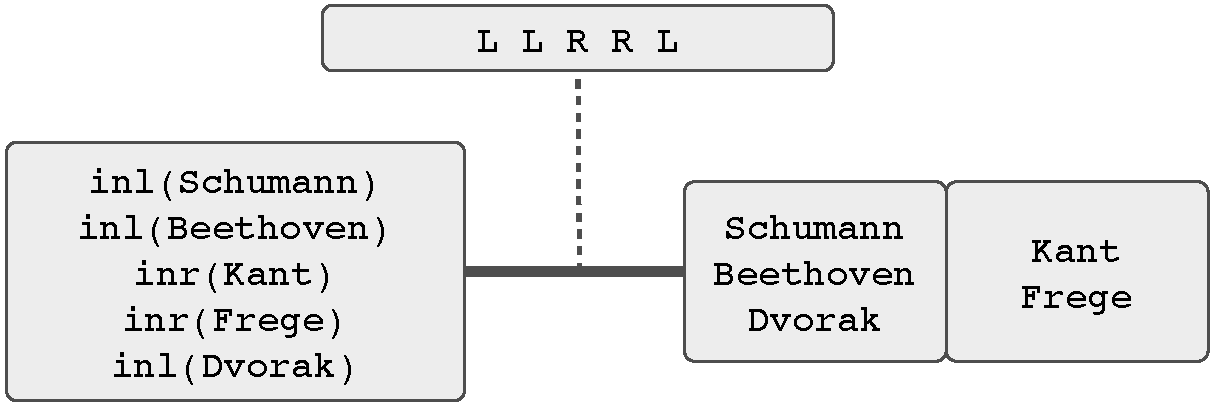
\includegraphics[width=75mm]{images/ex3-0.pdf}
        % \begin{tikzpicture}
        %     \draw
        %         node            (LSchumann)  {$\mlinl{\mbox{Schumann}}$}  (LSchumann)
        %         node[below=1ex] (LBeethoven) {$\mlinl{\mbox{Beethoven}}$} (LBeethoven)
        %         node[below=1ex] (LKant)      {$\mlinr{\mbox{Kant}}$}      (LKant)
        %         node[below=1ex] (LFrege)     {$\mlinr{\mbox{Frege}}$}     (LFrege)
        %         node[below=1ex] (LDvorak)    {$\mlinl{\mbox{Dvorak}}$}    (LDvorak)

        %         (LSchumann) +(7em, 0) node (CSchumann)  {$L$}
        %         (LBeethoven)+(7em, 0) node (CBeethoven) {$L$}
        %         (LKant)     +(7em, 0) node (CKant)      {$R$}
        %         (LFrege)    +(7em, 0) node (CFrege)     {$R$}
        %         (LDvorak)   +(7em, 0) node (CDvorak)    {$L$}

        %         (CKant)+(6.1em, 0)
        %         node            (RBeethoven) {Beethoven}
        %         node[above=1ex] (RSchumann)  {Schumann}
        %         node[below=1ex] (RDvorak)    {Dvorak}
        %         (RBeethoven)+(5em, 0) node {}
        %         node[above=0ex] (RKant)      {Kant}
        %         node[below=0ex] (RFrege)     {Frege}

        %         node[rbox,fit=(LDvorak) (LBeethoven) (LSchumann)]     (left)       {}
        %         node[rbox,fit=(CDvorak) (CSchumann)]                  (complement) {}
        %         node[rbox,fit=(RDvorak) (RSchumann) (RKant) (RFrege)] (right)      {}
        %         node[     fit=(RDvorak) (RBeethoven) (RSchumann)]     (right-inl)  {}
        %         node[     fit=(RKant) (RFrege)]                       (right-inr)  {}

        %         ($(right-inl.east)!0.5!(right-inr.west)$) node (right-center) {}
        %         (right-center |- right.north) -- (right-center |- right.south)

        %         node[below=2ex of complement]    (complement-label) {complement}
        %         (complement-label -| left)  node (left-label)       {left}
        %         (complement-label -| right) node (right-label)      {right}
        %     ;
        % \end {tikzpicture}
    \end{center}
    \caption{A consistent triple for the partition lens.}
    \label{fig:triple-partition}
    \vspace*{-2ex}
\end{figure}

As a warm-up, consider a simple edit: changing Dvorak's name to Dvo\v
r\'ak (with correct diacritics) in the left repository. The edit describing
this has the form \dissdis\mlmod5{\mlstayl{\d n}},\dissdis where $\d n$
describes the string edit to the
name. To translate this edit, we first need to 
translate the index $5$ to an index into the list of composers in the
right-hand repository (line \markref{rmodstay} in
Figure~\ifdissertation\ref{fig:definition-partition-part-2}\else\ref{fig:definition-partition}\fi).  We can do this by simply counting
how many composers 
appear up to and including Dvorak, that is, how many $L$ values appear in the
complement list up to index $5$---in this case, $3$.  We then wrap this
index up, along with the $\d n$ edit, in a new edit of the form
$\mlleft{\mlmod3{\d n}}$; the complement need not change because we
have not changed the structure of the lists. This pattern---count to
translate the index, then re-tag the edit appropriately---can be generalized
to all modifications that stay on the same side of the sum; the $\mlcount$
and $\mltag$ functions defined in
Figure~\ref{fig:definition-partition-supplementary} implement these two
steps.  

The left-to-right translation of other in-place modifications, insertions, and
deletions and the right-to-left translation of in-place modifications,
insertions, and deletions to either list are built from the same primitives, using
$\mlcount$ to translate indices and re-tagging edits with $\mltag$. 
%
In a few cases, we use some edit ``macros'': since insertions
and deletions always happen at the end of a list, we write $\mldelete'$ and
$\mlinsert'$ for edits that do some shuffling to ensure that the inserted or
deleted element moves to the appropriate position.

Perhaps the
most interesting of these is an in-place modification to the left repository
that switches sides of a sum (line~\markref{rmodswitch}).
%
For example, suppose we want to replace Beethoven with Plato. The edit to do
this has the form $\mlmod2{\mlswitch_{LR}(\d n)}$---that is, at position
$2$, switch from an $\mlinlx$ to an $\mlinrx$.  Here, the translated edit
must do \emph{four} things: delete Beethoven from the left list, insert a
new element into the right list, re-tag $\d n$ so that it changes the new
element to Plato, and finally fix up the complement to match the new
interleaving. As before, we can use $\mlcount$ to translate the position $2$
in the interleaved list into a position in the left list in the right
\replica. But then we hit a minor snag: deletions only occur at the end of a
list. The solution is to first reorder the list, so that Beethoven appears
at the end, then delete one element.
Figure~\ref{fig:definition-partition-supplementary} defines the $\ml{cycle}$
function, which constructs permutations to do this reordering. The
function $\ml{cycle}_p(n)$ permutes lists of size $n$ by moving position $p$
to the end of the list, and shifting all the other elements after $p$ down
one to fill in the resulting hole. For example, $\ml{cycle}_2(5)$ looks like
this:
\begin{center}
    \begin{tabular}{c|ccccc}
        $p$ & $1$ & $2$ & $3$ & $4$ & $5$ \\
        \hline
        $\ml{cycle}_2(5)(p)$ & $1$ & $3$ & $4$ & $5$ & $2$
    \end{tabular}
\end{center}
So, we can delete position $p$ by first reordering with
$\mlreorder{\ml{cycle}_p}$, then deleting one element with $\mldel1$. The
$\mldelete'(p)$ macro encapsulates this pattern; there is a similar pattern for
inserting a new element at position $p$ encapsulated by $\mlinsert'(p)$.
Finally, since position $2$ in the interleaved list corresponds to positions
$2$ and $1$ in the left and right non-interleaved lists, respectively, the
final edit can be written as
$\mlright{\mlmod1{\d n}}\,\mlright{\mlinsert'(1)}\,\mlleft{\mldelete'(2)}$.
To fix up the complement, we can simply set the flag at position $p$ to
match the new tag: in our case, position $2$ is now an $\mlinrx$, so we
should set $c_2=R$.

% TODO: perhaps interesting: inserts to the right often have a free choice
% about where to insert on the left; discuss this?

The most delicate cases involve translating reorderings.
Consider an edit to the right repository that swaps Schumann and
Dvorak.  One way to write this edit is in terms of
a function that swaps 
indices one and three for lists of size at least three (and does nothing on
lists of size smaller than three):
\[f(n)(p) = \cond{
    4-p & n \ge 3 \land p \in \{1, 3\} \\
    p & n < 3 \lor p \notin \{1, 3\}
    }\]
The edit itself is then $\mlleft{\mlreorder f}$. Our job is now to compute
some $f'$ for which $\mlreorder{f'}$ swaps $\mlinl{\mbox{Schumann}}$ and
$\mlinl{\mbox{Dvorak}}$ in the left repository
(line~\markref{lreorder}). There is one wrinkle: $f$ 
and $f'$ are parameterized by the length of the lists they permute.
Translating $f$ naively would therefore seem to require a way for $f'$ to
\emph{guess}  the number of composers in lists whose lengths do not
match that of the complement. Fortunately,
$f'$ need only behave correctly for exactly those lists that are consistent
with the current complement, for which our ``guess'' about how many
composers there are is guaranteed to be accurate.  So 
we need only construct a single permutation (and use, say, the
identity permutation for all inconsistent list lengths).
%
We use the $\mlcount$ function to construct this permutation.
It is convenient to derive an isomorphism between positions in the left
repository and positions tagged by which list they are indexing into in the
right repository; the $\mliso$ function shows how to use $\mlcount$ to do
this. In our example, the resulting isomorphism looks like this:
\begin{center}
\noindent \begin{tabular}{c|ccccc}
    left  & $1$ & $2$ & $3$ & $4$ & $5$ \\
    \hline
    right & $\mlinl 1$ & $\mlinl 2$ & $\mlinr 1$ & $\mlinr 2$ & $\mlinl 3$
\end{tabular}
\end{center}

We can use $f(3)$ as a permutation on the $\mlinlx$ elements, defining%
\ifdissertation:
\[g(p) = \cond{\mlinr{p'} & p = \mlinr{p'} \\
               \mlinl{f(3)(p')} & p = \mlinl{p'}}\]
\else\ $g(\mlinl p)=\mlinl{f(3)(p)}$ and $g(\mlinr p)=\mlinr p$. \fi Then, to find out
where position $p$ in the left repository should come from, we can simply
translate $p$ into an index into the right repository using $\mliso$, apply
$g$ to find out where that index came from, and translate back into the left
repository using $\mliso^{-1}$. Expanding the table above with these
translations yields:
\begin{center}
\begin{tabular}{@{}c|ccccc@{}}
    left & $1$ & $2$ & $3$ & $4$ & $5$ \\
    \hline
    $\mliso$ & $\mlinl 1$ & $\mlinl 2$ & $\mlinr 1$ & $\mlinr 2$ & $\mlinl 3$ \\
    $\mliso;g$ & $\mlinl 3$ & $\mlinl 2$ & $\mlinr 1$ & $\mlinr 2$ & $\mlinl 1$ \\
    $\mliso;g;\mliso^{-1}$ & $5$ & $2$ & $3$ & $4$ & $1$
\end{tabular}
\end{center}
This swaps indices $1$ and $5$, so our final $f'$ looks like:
\[f'(n)(p) = \cond{
    6-p & n = 5 \land p \in \{1,5\} \\
    p & n \ne 5 \lor p \notin \{1,5\}
    }\]

Translating a reordering of the left repository follows a similar path (line~\markref{rreorder}):
restrict the reordering to lists consistent with the current complement,
then compose the permutation with isomorphisms between the indices in the
two repositories. There is one subtlety here: a reordering of the list
in the left repository may shuffle which positions are $\mlinlx$'s and which
are $\mlinrx$'s. As a result, we must take care to construct \emph{two}
separate position isomorphisms: one for ``before'' the reordering, and one
for ``after\dotquote

% TODO: Somewhere in the above discussion we should probably try to give
% some intuition for what \mlcount does, since it's got such odd base cases.
% An attempt at English might go like this: Suppose we were to insert an L
% (respectively R) before index i in list c. How many Ls (respectively, Rs)
% would there be, up to this newly inserted item? These two numbers are the
% output of \mlcount(i,c).

\iffull
\begin{lemma}
    \label{lemma:unfold-mod-once}
    \[\mlmod p{\dv\CONS\dv s}z=\mlmod p\dv\mlmod p{\dv s}z\]
\end{lemma}

\begin{proof}
    Let $n=|z|$.  Either $p>n$ or not. If it is, then both sides are
    undefined; otherwise:
    \begin{align*}
        \mlmod p{\dv\CONS\dv s}z
            &= z[p \mapsto (\dv\CONS\dv s)z_p] \\
            &= z[p \mapsto \dv(\dv s\,z_p)] \\
            &= \mlmod p\dv(z[p \mapsto \dv s\,z_p]) \\
            &= \mlmod p\dv\mlmod p{\dv s}z
    \end{align*}
\end{proof}

\begin{lemma}
\label{lemma:high-level-delete}
If $1 \le p \le n$, then:
\[\mldelete'(p) \odot v = \blist v_1 \clist v_{p-1} \mlist v_{p+1} \clist v_n \elist\]
\end{lemma}

\begin{proof}
The only tricky part of this proof is evaluating $\ml{cycle}_p(n)$:
\begin{align*}
    \mldelete'(p) \odot v
        &= \blist\mldel 1\mlist\mlreorder{\ml{cycle}_p}\elist \odot v \\
        &= \blist\mldel 1\elist \odot \blist v_{\ml{cycle}_p(n)(1)} \clist v_{\ml{cycle}_p(n)(n)} \elist \\
        &= \blist\mldel 1\elist \odot \blist v_1 \clist v_{p-1} \mlist v_{p+1} \clist v_{n-1} \mlist v_p \elist \\
        &= \blist v_1 \clist v_{p-1} \mlist v_{p+1} \clist v_{n-1} \elist
\end{align*}
If $p=n$, then neither of the first two conditions in the definition of
$\ml{cycle}$ will ever be true, so $\ml{cycle}_p(n)(m)=m$, making the
evaluation given in these equations a special case where the interval from
$p+1$ to $n-1$ is empty and $v_p=v_n$. On the other hand, when $p<n$, the
value of $\ml{cycle}_p(n)$ is exactly in the form given here.
\end{proof}

\begin{lemma}
\label{lemma:high-level-insert}
When $1 \le p \le n+1$:
\[\mlinsert'(p) \odot \blist v_1 \clist v_n \elist =
    \blist v_1 \clist v_{p-1} \mlist \init \mlist v_p \clist v_n \elist\]
\end{lemma}

\begin{proof} Set $v_{n+1}=\init$ so that:
\begin{align*}
    \mlinsert'(p) \odot v_1 \cdots v_n
        &= \mlreorder{\lambda n.\ \ml{cycle}_p(n)^{-1}}\mlins 1 \odot \blist v_1 \clist v_n \elist \\
        &= \mlreorder{\lambda n.\ \ml{cycle}_p(n)^{-1}} \odot \blist v_1 \clist v_n\mlist\init\elist \\
        &= \mlreorder{\lambda n.\ \ml{cycle}_p(n)^{-1}} \odot \blist v_1 \clist v_{n+1} \elist \\
        &= \blist v_{\ml{cycle}_p(n+1)^{-1}(1)} \clist v_{\ml{cycle}_p(n+1)^{-1}(n+1)} \elist \\
        &= \blist v_1 \clist v_{p-1} \mlist v_{n+1} \mlist v_p \clist v_n \elist \\
        &= \blist v_1 \clist v_{p-1} \mlist \init \mlist v_p \clist v_n \elist
\end{align*}
As with Lemma~\ref{lemma:high-level-delete}, the only tricky part is arguing
that this evaluation of $\ml{cycle}_p$ is correct, and the argument is
similar to the one given there, but in reverse.
\end{proof}

\begin{lemma}
\label{lemma:lefts-rights-homomorphism}
The $\ml{lefts}$ and $\ml{rights}$ functions are list homomorphisms, that
is,
\[\ml{lefts}(vw)=\ml{lefts}(v)\ml{lefts}(w),\]
and similarly for $\ml{rights}$.
\end{lemma}

\begin{proof}
We will show the proof for $\ml{lefts}$. We argue by induction on $v$. In
the base case, $v=\NIL$, and:
\begin{align*}
    \ml{lefts}(vw)
        &= \ml{lefts}(w) \\
        &= \NIL\ml{lefts}(w) \\
        &= \ml{lefts}(\NIL)\ml{lefts}(w) \\
        &= \ml{lefts}(v)\ml{lefts}(w)
\end{align*}
Otherwise, $v=v_1 \CONS v'$, we know from the induction hypothesis that
$\ml{lefts}(v'w)=\ml{lefts}(v')\ml{lefts}(w)$, and by case analysis either
$v_1=\mlinl x$ or $v_1=\mlinr y$. In the former case:
\begin{align*}
    \ml{lefts}(vw)
        &= \ml{lefts}(\mlinl x \CONS v'w) \\
        &= x\CONS\ml{lefts}(v'w) \\
        &= x\CONS\ml{lefts}(v')\ml{lefts}(w) \\
        &= \ml{lefts}(\mlinl x \CONS v')\ml{lefts}(w) \\
        &= \ml{lefts}(v)\ml{lefts}(w)
\end{align*}
In the latter:
\begin{align*}
    \ml{lefts}(vw)
        &= \ml{lefts}(\mlinr y \CONS v'w) \\
        &= \ml{lefts}(v'w) \\
        &= \ml{lefts}(v')\ml{lefts}(w) \\
        &= \ml{lefts}(\mlinr y \CONS v')\ml{lefts}(w) \\
        &= \ml{lefts}(v)\ml{lefts}(w)
\end{align*}
\end{proof}

\begin{lemma}
\label{lemma:iso-coherent}
The isomorphism produced by $\mliso$ is coherent in the following sense.
Choose arbitrary $v\in(X+Y)\LIST$ and let $c=\map_{\ml{tagof}}(v)$ be
the list of tags of $v$. If $\mliso(c)(p)=\mlinl{p'}$ then
$\mlinl{\ml{lefts}(v)_{p'}}=v_p$ and likewise if $\mliso(c)(p)=\mlinr{p'}$
then $\mlinr{\ml{rights}(v)_{p'}}=v_p$.
\end{lemma}

\begin{proof}
Suppose there are $n_L$ copies of $L$ and $n_R$ copies of $R$ in $\blist c_1
\clist c_{p-1} \elist$ and $p \le n+1$. Then it is easy to show (by
induction on $c$) that $\ml{count}(p,\blist c_1 \clist c_n
\elist)=(1+n_L,1+n_R)$. Inspecting the definition of $\mliso$, it is
therefore clear that $\mliso(c)(p)=\mlinl{p'}$ exactly when $c_p=L$ and
there are $p'$ copies of $L$ in $\blist c_1 \clist c_p \elist$. This implies
there are exactly $p'$ elements tagged $\ml{inl}$ in $\blist v_1 \clist v_p
\elist$ (and that $v_p$ itself is tagged $\ml{inl}$), hence that
$\mlinl{\ml{lefts}(v)_{p'}}=v_p$.

The argument that $\mliso$ is coherent with $\ml{rights}$ is similar.
\end{proof}

\begin{corollary}
\label{lemma:iso-tag-index}
If $c=\map_{\ml{tagof}}(v)$ and $1 \le p \le |v|$, then
\[\ml{tagof}(v_p)=\ml{tagof}(\mliso(c)(p)).\]
\end{corollary}

\begin{lemma}
\label{lemma:iso-monotonic}
Suppose $\mliso(c)(m)=\mlinl n$ (respectively, $\mlinr n$) and
$\mliso(c)(m')=\mlinl{n'}$ (resp. $\mlinr{n'}$). Then $m<m'$ if and only if
$n<n'$.
\end{lemma}

\begin{proof}
    As shown in the proof of Lemma~\ref{lemma:iso-coherent}, we have
    $\mliso(c)(m)=\mlinl n$ exactly when $c_m=L$ and there are $n$ copies of
    $L$ in $\blist c_1 \clist c_m\elist$. A similar statement relates $m'$
    and $n'$. Since $\blist c_1 \clist c_m \elist$ and $\blist c_1 \clist
    c_{m'} \elist$ share a common prefix, if one has more copies of $L$ than
    the other then it must be longer---that is, $n'>n$ implies $m'>m$. On
    the other hand, since $c_m=c_{m'}=L$, if one is longer than the other
    than it definitely has more copies of $L$---that is, $m'>m$ implies
    $n'>n$.
\end{proof}

\begin{theorem}
The $\partition$ operation defined in \partitionfigures is indeed a
symmetric edit lens.
\label{goodlens:partition}
\end{theorem}

\begin{proof}
According to Definition~\ref{defn:lens}, we must show three things.  First,
$\partition.\dputr$ and $\partition.\dputl$ must be stateful monoid
homomorphisms; since the edit monoid for the list module is freely
generated and the two functions in question are defined by specification,
this is immediate.  Second, the initial state \[(\init_{(X \oplus
  Y)\LIST}, \NIL, \init_{X\LIST \otimes Y\LIST})\] must be an element of $K$;
this is easily verified from the definitions of the initial elements of the
list and product modules.  And third, the $\dputr$ and $\dputl$ operations
must preserve consistent states; this is where some work is required.  We
show that $\dputr\gen$ and $\dputl\gen$ respect $K$; since $\dputr$ and $\dputl$
are defined by specification from these, the fact that they respect $K$
follows by induction on the number of atomic edits they are handed.

\newcommand{\partitiondputrproof}{
We are given some $\dz \in G^{\mathrm{list}}_{X \oplus Y}$ such that
$\dz\;z$ is defined. We can define $(\dz',c')=\dputr\gen(\dz,c)$; then we
must show that $\dz'(x,y)$ is defined and that $(\dz\;z,c',\dz'(x,y)) \in
K$. We proceed by induction on the size of $\dz$.
\begin{trivlist}
\item {\bf Case \markref{rmodbigp}:}
    $\dv \in X \oplus Y$ and $\dz=\mlmod p\dv$ and $p > |c|$.

    \noindent
    Since $|z|=|c|$, we conclude that $\dz\;z$ is undefined, a
    contradiction.

\item {\bf Case \markref{rmodempty}:}
    $\dz=\mlmod p\NIL$ and $1 \le p \le |c|$.

    \noindent
    We calculate:
    \begin{align*}
        \dz' &= \NIL \\
        c' &= c \\
        \dz\;z &= z \\
        \dz'(x,y) &= (x,y)
    \end{align*}
    So $(\dz\;z,c',\dz'(x,y)) \in K$ by assumption:
    $(z,c,(x,y)) \in K$.

\item {\bf Case \markref{rmodcons}:}
    We have all of the following:
    \begin{align}
        \dv &\in G^\oplus_{X,Y} \\
        \dv s &\in \D(X\oplus Y) \\
        \dz &= \mlmod p{\dv\CONS\dv s} \\
        1 &\le p \le |c| \\
        1 &< n \\
        (d,c'') &= \dputr\gen(\mlmod p{\dv s},c) \label{eq:IH-1} \\
        (d',c') &= \dputr\gen(\mlmod p\dv,c'') \label{eq:IH-2} \\
        \dz' &= d'\;d
    \end{align}
    By Lemma~\ref{lemma:unfold-mod-once} and the assumption that $\mlmod
    p{\dv\CONS\dv s}z$ is defined, we know $\mlmod p\dv(\mlmod p{\dv s}z)$ is
    defined, and hence $\mlmod p{\dv s}z$ is defined. The induction
    hypothesis for equation~\ref{eq:IH-1} therefore tells us that $d\;(x,y)$
    is defined and that
    \[(\mlmod p{\dv s}z,c'',d\;(x,y)) \in K.\]
    Again appealing to the induction hypothesis, this time for
    equation~\ref{eq:IH-2}, we also know that $d'\;(d\;(x,y))$ is defined and
    \[(\mlmod p\dv(\mlmod p{\dv s}z),c',d'\;(d\;(x,y))) \in K.\]
    By one final appeal to Lemma~\ref{lemma:unfold-mod-once}, we therefore
    conclude that
    \[(\dz\;z,c',\dz'(x,y)) \in K\]
    as desired.

\item {\bf Case \markref{rmodswitch}:}
    We have:
    \begin{align*}
        \dz &= \mlmod p{\mlswitch_{jk}(\dv)} \\
        1 &\le p \le |c| \\
        \dv &\in \partial X\mbox{ when }k = L \\
        \dv &\in \partial Y\mbox{ when }k = R \\
        \dz' &= d_2d_1d_0 \\
        c' &= c[p \mapsto k] \\
        d_0 &= \map_{\lambda d.\,\ml{tag}(j,d)}(\mldelete'(p_j)) \\
        d_1 &= \map_{\lambda d.\,\ml{tag}(k,d)}(\mlinsert'(p_k)) \\
        d_2 &= \ml{tag}(k,\mlmod{p_k}\dv) \\
        (p_L,p_R) &= \mlcount(p,c)
    \end{align*}
    Let us consider the case when $j=k=L$, whose argument is representative
    of the other cases.

    Since $\dz\;z$ is defined, we know that $z_p = \mlinl v$ for some $v \in
    X$. Taking $v'=\dv\;\init_X$, we can now compute:
    \begin{align*}
        \map_{\ml{tagof}}(\dz\;z)
            &= \map_{\ml{tagof}}(z[p\mapsto\mlinl{v'}]) \\
            &= \map_{\ml{tagof}}(\blist z_1\clist z_{p-1}\elist)\;
               \blist k\elist\;
               \map_{\ml{tagof}}(\blist z_{p+1}\clist z_n\elist)\\
            &= \blist c_1\clist c_{p-1}\mlist k\mlist c_{p+1}\clist c_n \elist\\
            &= c[p \mapsto k] \\
            &= c'
    \end{align*}
    The second line follows from the first because \map is a list
    homomorphism.  Hence $\dputr\gen$ maintains consistency of $c$ in this
    case; it remains to show that $\dputr\gen$ maintains consistency of the
    output. We calculate the effects of $\dz$ and $\dz'$, starting with
    $\dz'$:
    \begin{align*}
        \dz'\;(x,y)
            &= d_2d_1d_0(x,y) \\
            &= d_2d_1(\map_{\lambda d.\ml{tag}(j,d)}(\mldelete'(p_j)))(x,y) \\
            &= d_2d_1(\map_{\ml{left}}(\mldelete'(p_L)))(x,y) \\
            &= d_2d_1(\mldelete'(p_L)x,y) \\
            &= d_2(\map_{\lambda d.\ml{tag}(k,d)}(\mlinsert'(p_k)))(\mldelete'(p_L)x,y) \\
            &= d_2(\map_{\ml{left}}(\mlinsert'(p_L)))(\mldelete'(p_L)x,y) \\
            &= d_2(\mlinsert'(p_L)\mldelete'(p_L)x,y) \\
            &= \mltag(k,\mlmod(p_k,\dv))(\mlinsert'(p_L)\mldelete'(p_L)x,y) \\
            &= (\mlmod{p_L}\dv\mlinsert'(p_L)\mldelete'(p_L)x,y)
    \end{align*}
    We can use Lemmas~\ref{lemma:high-level-delete}
    and~\ref{lemma:high-level-insert} to simplify:
    \begin{align*}
        \dz'\;(x,y)
            &= (\mlmod{p_L}\dv\mlinsert'(p_L)\mldelete'(p_L)\blist x_1\clist x_{n_L}\elist,y) \\
            &= (\mlmod{p_L}\dv\mlinsert'(p_L)\blist x_1\clist x_{p_L-1}\mlist x_{p_L+1}\clist x_{n_L}\elist,y) \\
            &= (\mlmod{p_L}\dv\blist x_1\clist x_{p_L-1}\mlist\init_X\mlist x_{p_L+1}\clist x_{n_L}\elist,y) \\
            &= (\blist x_1\clist x_{p_L-1}\mlist v'\mlist x_{p_L+1}\clist x_{n_L}\elist,y) \\
            &= (x[p_L\mapsto v'], y)
    \end{align*}
    We now make some observations about the effects of $\dz$, making crucial
    use of Lemma~\ref{lemma:lefts-rights-homomorphism}:
    \begin{align*}
        \ml{rights}(\dz\;z)
            &= \ml{rights}(\blist z_1 \clist z_{p-1} \mlist \mlinl{v'} \mlist z_{p+1} \clist z_n \elist) \\
            &= \ml{rights}(\blist z_1 \clist z_{p-1}\elist) \ml{rights}(\mlinl{v'}) \ml{rights}(\blist z_{p+1} \clist z_n \elist) \\
            &= \ml{rights}(\blist z_1 \clist z_{p-1}\elist) \ml{rights}(\mlinl{v}) \ml{rights}(\blist z_{p+1} \clist z_n \elist) \\
            &= \ml{rights}(\blist z_1 \clist z_{p-1}\elist) \ml{rights}(z_p) \ml{rights}(\blist z_{p+1} \clist z_n \elist) \\
            &= \ml{rights}(\blist z_1 \clist z_{p-1} \mlist z_p \mlist z_{p+1} \clist z_n \elist) \\
            &= \ml{rights}(z) \\
            &= y
    \end{align*}
    We now observe that Lemma~\ref{lemma:iso-coherent} implies that
    $\ml{lefts}(\blist z_1 \clist z_{p-1} \elist)=\blist x_1 \clist
    x_{p_L-1} \elist$ and likewise that $\ml{lefts}(\blist z_{p+1} \clist
    z_n \elist)=\blist x_{p_L+1} \clist x_{n_L} \elist$.
    \begin{align*}
        \ml{lefts}(\dz\;z)
            &= \ml{lefts}(z[p \mapsto \mlinl{v'}]) \\
            &= \ml{lefts}(\blist z_1 \clist z_{p-1} \elist)\ml{lefts}(\mlinl{v'})\ml{lefts}(\blist z_{p+1} \clist z_n \elist) \\
            &= \blist x_1\clist x_{p_L-1}\mlist v'\mlist x_{p_L+1}\clist x_{n_L}\elist \\
            &= x[p_L\mapsto v']
    \end{align*}
    Taken together, these last three computations show that
    \[\dz'\;(x,y) = (\ml{lefts}(\dz\;z),\ml{rights}(\dz\;z))\]
    which is just what we needed.

\item {\bf Case \markref{rmodstay}:} Let us consider specifically the case
    where $j=L$; the argument for $j=R$ is very similar. Then we have
    \begin{align*}
        \dz &= \mlmod p{\mlstayl\dv} \\
        \dz' &= \mlonl{\mlmod{p_L}\dv} \\
        (p_L,p_R) &= \mlcount(p,c)
    \end{align*}
    Moreover, since $\dz\;z$ is defined, we know that there is some $v \in
    X$ for which $\dv\;v$ is defined such that $z_p = \mlinl v$ and, by
    appeal to Lemma~\ref{lemma:iso-coherent}, we know in particular that
    $v=\ml{lefts}(z)_{p_L}=x_{p_L}$. Hence $\dz'\;(x,y)$ is defined.

    We now observe that $\mlmod p{\mlstayl\dv}$ does not change any tags or
    any non-$\ml{inl}$ values, so $\map_{\ml{tagof}}(\dz\;z) =
    \map_{\ml{tagof}}(z) = c$ and $\ml{rights}(\dz\;z) = \ml{rights}(z)
    = y$. Furthermore:
    \begin{align*}
        \ml{lefts}(\dz\;z)
        &= \ml{lefts}(\mlmod p{\mlstayl\dv}\;z[p \mapsto \mlinl{x_{p_L}}]) \\
        &= \ml{lefts}(z[p\mapsto\mlinl{\dv\;x_{p_L}}]) \\
        &= x[p_L\mapsto \dv\;x_{p_L}] \\
        &= \mlmod{p_L}{\dv}\;x
    \end{align*}
    That is, $\dz\;z$ and $\dz'\;(x,y)=(\mlmod{p_L}\dv\;x,y)$ are synchronized as desired.

\item {\bf Case \markref{rmodfail}:}
    When $\dz=\mlmod p\fail$ there is nothing to prove, because the
    assumption that the edit application is defined is immediately
    contradicted.

\item {\bf Case \markref{rins}:}
    \begin{align*}
        \dz &= \mlins i \\
        \dz' &= \mlonl{\mlins i}  \\
        c' &= \mlins i\,c
    \end{align*}

    \noindent
    We calculate:
    \begin{align*}
        \dz\;z &= z\replicate i{\init_{X\oplus Y}}
\\
               &= z\replicate i{\mlinl{\init_X}}
\\
        \dz'(x,y) &= (x\replicate i{\init_X},\, y)
\\
        c' &= c\replicate iL
    \end{align*}
    Now, since \map is a list homomorphism, we have:
    \begin{align*}
        \map_\ml{tagof}(\dz\;z)
            &= \map_\ml{tagof}(z)\map_\ml{tagof}\left(\replicate i{\mlinl{\init_X}}\right) \\
            &= c\replicate iL \\
            &= c'
    \end{align*}
    Likewise, by Lemma~\ref{lemma:lefts-rights-homomorphism}:
    \begin{align*}
        \ml{lefts}(\dz\;z)
            &= \ml{lefts}(z)\ml{lefts}\left(\replicate i{\mlinl{\init_X}}\right) \\
            &= x\replicate i{\init_X} \\
        \ml{rights}(\dz\;z)
            &= \ml{rights}(z)\ml{rights}\left(\replicate i{\mlinl{\init_X}}\right) \\
            &= y
    \end{align*}
    These latter two computations amount to showing that
    \dissdis\dz'(x,y)=(\ml{lefts}(\dz\;z),\ml{right}(\dz\;z))\dissdis which, together with
    the observation above that $\map_\ml{tagof}(\dz\;z)=c'$, shows that
    $\dputr\gen$ preserves consistency in this case.

\item {\bf Case \markref{rdel}:}
    \begin{align*}
        \dz &= \mldel i \\
        \dz' &= \mlright{\mldel{n_L-1}}\mlleft{\mldel{n_R-1}} \\
        (n_L,n_R) &= \mlcount(i+1,\mlreverse(c))
    \end{align*}
    (Take careful notice of the definition of $n_L$ and $n_R$ here: it
    differs from the convention established at the beginning of the proof!
    We will use these local definitions for the remainder of this case.)

    The interesting thing to prove is that $\ml{lefts}(\mldel i\;z) =
    \mldel{n_L-1}\ml{lefts}(z)$ (and similarly for $\ml{rights}$). We
    proceed by an inner induction on $i$.

    When $i=0$, we have $\ml{lefts}(\mldel 0\;z)=\ml{lefts}(z)$ and
    \[(n_L,n_R) = \mlcount(1,\mlreverse(c)) = (1,1)\] so that
    $\mldel{n_L-1}\ml{lefts}(z)=\mldel0\ml{lefts}(z)=\ml{lefts}(z)$.

    Suppose $i>0$. Define the abbreviation $c^r=\mlreverse(c)$.
    Then the induction hypothesis says that
    \[\ml{lefts}(\mldel{i-1}\;z)=\mldel{\mlfst(\mlcount(i,c^r))-1}\ml{lefts}(z).\]
    Now, either $c^r_i=L$ or $c^r_i=R$. If the former, then
    $z_{n-i+1}=\mlinl x$ for some $x$ and:
    \begin{align*}
        \mldel{n_L-1}\ml{lefts}(z)
        &= \mldel{\mlfst(\mlcount(i+1,c^r))-1}\ml{lefts}(z) \\
        &= \mldel{1+\mlfst(\mlcount(i,c^r))-1}\ml{lefts}(z) \\
        &= \mldel1\mldel{\mlfst(\mlcount(i,c^r))-1}\ml{lefts}(z) \\
        &= \mldel1\ml{lefts}(\mldel{i-1}\;z) \\
        &= \mldel1\ml{lefts}(\blist z_1 \clist z_{n-i}\mlist\mlinl x\elist) \\
        &= \mldel1(\ml{lefts}(\blist z_1 \clist z_{n-i}\elist)x) \\
        &= \ml{lefts}(\blist z_1 \clist z_{n-i}\elist) \\
        &= \ml{lefts}(\mldel i\;z)
    \end{align*}
    Otherwise, $z_{n-i+1}=\mlinr y$ for some $y$ and:
    \begin{align*}
        \mldel{n_L-1}\ml{lefts}(z)
        &= \mldel{\mlfst(\mlcount(i+1,c^r))-1}\ml{lefts}(z) \\
        &= \mldel{\mlfst(\mlcount(i,c^r))-1}\ml{lefts}(z) \\
        &= \ml{lefts}(\mldel{i-1}\;z) \\
        &= \ml{lefts}(\blist z_1 \clist z_{n-i}\mlist\mlinr y\elist) \\
        &= \ml{lefts}(\blist z_1 \clist z_{n-i}\elist) \\
        &= \ml{lefts}(\mldel i\;z)
    \end{align*}
    as desired.

    A similar argument shows that:
    \[\ml{rights}(\mldel i\;z) = \mldel{n_R-1}\ml{rights}(z)\]

\item {\bf Case \markref{rreorder}:}
    The main idea of the proof for this case is to observe that $c$ contains
    enough information to deduce the length of $x$, $y$, and $z$, and in
    particular which index the various $\ml{reorder}$ edits will be
    specialized to during edit application. We can focus on these indices.
    (We will see that the somewhat strange-looking clause defining $f_k(n
    \ne n_k) = \lambda p.\; p$ is never used -- the lens could use any
    automorphism on $\{1,\ldots,n\}$ in place of the identity there.)

    Because the application of $\dz$ and $\dz'$ are always defined, we need
    only show that the new complement and the output edits are consistent
    with the input edits. We begin by showing the new complement is
    consistent with $\dz\;z$.

    \begin{align}
        \map_{\ml{tagof}}(\dz\;z)
            &= \map_{\ml{tagof}}(\blist z_{f(n)(1)}\clist z_{f(n)(n)}\elist)
            \label{eq:reorder-z} \\
            &= \blist\map_{\ml{tagof}}(z)_{f(n)(1)}\clist\map_{\ml{tagof}}(z)_{f(n)(n)}\elist
            \label{eq:float-index} \\
            &= \blist c_{f(n)(1)} \clist c_{f(n)(n)} \elist
            \label{eq:def-c} \\
            &= \mlreorder f\;c
            \label{eq:def-reorder}
    \end{align}

    Equation~\ref{eq:reorder-z} follows by definition of edit application in
    the list module (and because $|z|=|c|=n$); equation~\ref{eq:float-index}
    is a special property of \map; equation~\ref{eq:def-c} by
    definition of $c$; and equation~\ref{eq:def-reorder} by the definition
    of $\ml{reorder}$'s edit application.

    We will now show that $\ml{lefts}(\dz\;z)=\mlreorder{f_L}\;x$. A similar
    argument to the following also shows that
    $\ml{rights}(\dz\;z)=\mlreorder{f_R}\;y$, and these two facts together
    will conclude the proof (since
    $\dz'\;(x,y)=(\mlreorder{f_L}\;x,\mlreorder{f_R}\;y)$). By the above
    fact about $c'$ and Lemma~\ref{lemma:iso-coherent}:
    \begin{align}
        \mlinl{\ml{lefts}(\dz\;z)_i}
            &= (\dz\;z)_{\mliso^{-1}(c')(\mlinl i)}
            \label{eq:lefts-lemma}\\
            &= (\dz\;z)_{h'^{-1}(\mlinl i)}
            \label{eq:def-h'}\\
            &= z_{f(n)(h'^{-1}(\mlinl i))}
            \label{eq:apply-reordering-to-def-h'}\\
            &= \mlinl{\ml{lefts}(z)_{\mluntag(\mliso(c)(f(n)(h'^{-1}(\mlinl i))))}}
            \label{eq:lefts-unlemma}\\
            &= \mlinl{\ml{lefts}(z)_{\mluntag(h(f(n)(h'^{-1}(\mlinl i))))}}
            \label{eq:def-h}\\
            &= \mlinl{\ml{lefts}(z)_{(\ml{inl};h'^{-1};f(n);h;\mluntag)(i)}}
            \label{eq:semi-syntax}\\
            &= \mlinl{\ml{lefts}(z)_{(\ml{inl};h'';\mluntag)(i)}}
            \label{eq:def-h''}\\
            &= \mlinl{\ml{lefts}(z)_{f_L(n_L)(i)}}
            \label{eq:def-fL}\\
        \ml{lefts}(\dz\;z)_i &= \ml{lefts}(z)_{f_L(n_L)(i)}
            \label{eq:uninl}
    \end{align}
    Equation~\ref{eq:lefts-lemma} is a straightforward application of
    Lemma~\ref{lemma:iso-coherent}; equation~\ref{eq:def-h'} folds the
    definition of $h'$; and equation~\ref{eq:apply-reordering-to-def-h'} applies
    edit $\dz$. Equation~\ref{eq:lefts-unlemma} applies
    Lemma~\ref{lemma:iso-coherent} again, but with the knowledge that the
    tag of the previous line is $\ml{inl}$ (because that is the left-hand
    side of the equality we have already proved). Equations~\ref{eq:def-h},
    \ref{eq:semi-syntax}, \ref{eq:def-h''}, and~\ref{eq:def-fL} just rewrite
    the equation by folding the definitions of $h$, $h''$, and $f_L$ and
    rewriting explicit function application as the application of a function
    composition. The final equation~\ref{eq:uninl} holds by injectivity of
    $\ml{inl}$.

    Now, since $x=\ml{lefts}(z)$ and $|x|=n_L$, we can conclude that
    $\ml{lefts}(\dz\;z)=\mlreorder{f_L}\;x$ as desired.

\item {\bf Case \markref{rfail}:} As in Case~\markref{rmodfail}, there is
    nothing to prove, as the assumption that the edit application is defined
    is immediately contradicted.

\end{trivlist}
}
\newcommand{\partitiondputlproof}{
We will give the proofs for atomic edits of the form $\mlonl\dx$; the proofs
for edits of the form $\mlonr\dy$ are similar. Choose $\dx \in
G^{\mathrm{list}}_X$ such that $\dx\;x$ is defined. We define
$(\dz,c')=\dputl\gen(\mlonl\dx,c)$ and must show that $\dz\;z$ is defined and
that $(\dz\;z,c',(\dx\;x,y)) \in K$. We proceed by induction on the size of
$\dx$.

\begin{trivlist}

\item {\bf Case \markref{lmod}:} In this case, we have the following
    equalities:
    \begin{align*}
        \dx &= \mlmod p\dv \\
        \dz &= \mlmod{p'}{\mlstayl\dv} \\
        c' &= c \\
        p' &= \mliso(c)^{-1}(\mlinl p)
    \end{align*}
    By Lemma~\ref{lemma:iso-coherent},
    $z_{p'}=\mlinl{\ml{lefts}(z)_p}=\mlinl{x_p}$. This gives us enough to
    know that $\dz\;z$ is defined and in fact that
    \begin{align*}
        \dz\;z
            &= z[p' \mapsto \mlstayl\dv\;z_{p'}] \\
            &= z[p' \mapsto \mlstayl\dv\;\mlinl{x_p}] \\
            &= z[p' \mapsto \mlinl{\dv\;x_p}]
    \end{align*}
    Since none of the tags of $z$ changes during this operation, this makes
    the computation of $\ml{lefts}$, $\ml{rights}$, and $\map_{\ml{tagof}}$
    easy:
    \begin{align*}
        \map_{\ml{tagof}}(\dz\;z)
            &= \map_{\ml{tagof}}(z) \\
            &= c \\
            &= c' \\
        \ml{rights}(\dz\;z)
            &= \ml{rights}(z) \\
            &= y \\
        \ml{lefts}(\dz\;z)
            &= \ml{lefts}(z)[p \mapsto \dv\;x_p] \\
            &= x[p \mapsto \dv\;x_p] \\
            &= \dx\;x
    \end{align*}
    These three computations establish that $(\dz\;z,c',(\dx\;x,y)) \in K$,
    as desired.

\item {\bf Case \markref{lreorder}:} We have a slew of equalities in hand to
    begin with. We have some chosen $f$ and three main equalities:
    \begin{align*}
        \dx &= \mlreorder f \\
        \dz &= \mlreorder{f'} \\
        c' &= c
    \end{align*}
    These depend on the additional definitions:
    \begin{align*}
        g(\mlinr p) &= \mlinr p &
        f'(n \ne |c|) &= \lambda p.\,p \\
        g(\mlinl p) &= \mlinl{f(n_L)(p)} &
        f'(|c|) &= h;g;h^{-1} \\
        h &= \mliso(c)
    \end{align*}

    We first observe that $\mlreorder{f'}$ does not affect tags at all. To
    be precise, for $1 \le p \le n$, we have:
    \begin{align}
        \ml{tagof}((\mlreorder{f'}\;z)_p)
            &= \ml{tagof}(z_{(h;g;h^{-1})(p)})
            \label{eq:def-reorder-f} \\
            &= \ml{tagof}((h;g;h^{-1};h)(p))
            \label{eq:swap-index-to-iso} \\
            &= \ml{tagof}((h;g)(p))
            \label{eq:elim-iso} \\
            &= \ml{tagof}(h(p))
            \label{eq:inspect-g} \\
            &= \ml{tagof}(z_p)
            \label{eq:swap-iso-to-index}
    \end{align}
    Equation~\ref{eq:def-reorder-f} follows from the definition of $f'$ and
    edit application. Equation~\ref{eq:swap-index-to-iso} is an application
    of Corollary~\ref{lemma:iso-tag-index}; we can then simplify
    significantly in equations~\ref{eq:elim-iso} and~\ref{eq:inspect-g}
    because $h$ is an isomorphism and $g$ does not modify tags, as is
    evident from its definition. A second application of
    Corollary~\ref{lemma:iso-tag-index}, this time ``in reverse'', gives us
    the final equation~\ref{eq:swap-iso-to-index}. We conclude that
    \[\map_{\ml{tagof}}(\dz\;z) = \map_{\ml{tagof}}(z) = c = c',\]
    part of what we need to show that $(\dz\;z,c',(\dx\;x,y))\in K$. (It
    also means that $h$ is the appropriate isomorphism to use when applying
    Lemma~\ref{lemma:iso-coherent} to $\dz\;z$.)

    Let us now turn our attention to showing that $\dz\;z$ and $\dx\;x$ have
    the appropriate relationship. We reason as follows:
    \begin{align}
        \mlinl{\ml{lefts}(\dz\;z)_p}
            &= (\dz\;z)_{h^{-1}(\mlinl p)}          \label{eq:lreorder-x-iso} \\
            &= z_{(h^{-1};h;g;h^{-1})(\mlinl p)}    \label{eq:lreorder-x-reorder} \\
            &= z_{(g;h^{-1})(\mlinl p)}             \label{eq:lreorder-x-elim-iso} \\
            &= z_{h^{-1}(f(n_L)(p))}                \label{eq:lreorder-x-g} \\
            &= \mlinl{\ml{lefts}(z)_{f(n_L)(p)}}    \label{eq:lreorder-x-iso2}
    \end{align}
    Equation~\ref{eq:lreorder-x-iso} is an application of
    Lemma~\ref{lemma:iso-coherent}. The next three equations,
    \ref{eq:lreorder-x-reorder} through \ref{eq:lreorder-x-g}, are mere
    computations that invoke the definitions of $\dz$, edit application, and
    $g$. The final equation~\ref{eq:lreorder-x-iso2} follows from the
    previous by Lemma~\ref{lemma:iso-coherent}. A similar argument to the
    above, differing only in line~\ref{eq:lreorder-x-g} where the definition
    of $g$ is used, shows that
    \[\mlinr{\ml{rights}(\dz\;z)_p} = \mlinr{\ml{rights}(z)_p}.\]

    We can therefore conclude that $\ml{lefts}(\dz\;z) = \dx\;\ml{lefts}(z)
    = \dx\;x$ and that $\ml{rights}(\dz\;z) = \ml{rights}(z) = y$, that is,
    that $(\dz\;z,c',(\dx\;x,y))\in K$ as desired.

\item {\bf Case \markref{lins}:} We know $\dx = \mlins i$ and $\dz = \mlins
    i$ and $c' = \mlins i\; c$. We compute:
    \begin{align*}
        \map_{\ml{tagof}}(\dz\;z)
            &= \map_{\ml{tagof}}(z \replicate i{\init_{X \oplus Y}}) \\
            &= \map_{\ml{tagof}}(z)\map_{\ml{tagof}}(\replicate i{\init_{X \oplus Y}}) \\
            &= c\replicate iL \\
            &= \mlins i\;c \\
            &= c'
    \end{align*}
    There's a slight left-bias here; in the right- version of this proof, we
    find that $\dputl\gen$ would have to produce a $c'$ with many replicated
    $R$s instead of $L$s, and so would not have quite as compact a syntax
    for this output.
    % TODO: does this mean we should explicitly give \dputl\gen(\mlonr{\mlins
    % i}) when defining the partition lens above?

    \begin{align*}
        \ml{lefts}(\dz\;z)
            &= \ml{lefts}(z\replicate i{\init_{X \oplus Y}}) \\
            &= \ml{lefts}(z)\ml{lefts}(\replicate i{\init_{X \oplus Y}}) \\
            &= x\replicate i{\init_X} \\
            &= \mlinsert(i)\;x \\
            &= \dx\;x
    \end{align*}
    Again, the left-bias means the right- version of this proof relies on
    $\dputl\gen$ being slightly more complicated for the right- analog. In
    particular, $\dputl\gen$ would need to output an edit which did the
    insertion above followed by a series of modifications that turned the
    $i$ final copies of $\mlinl{\init_X}$ into $i$ copies of
    $\mlinr{\init_Y}$.

    A similar computation to the previous one shows that
    $\ml{rights}(\dz\;z)=\ml{rights}(z)=y$.
%
    This concludes the proof of this case, since our three computations have
    shown that $(\dz\;z,c',(\dx\;x,y)) \in K$.

\item {\bf Case \markref{ldel0}:} We have $\dx = \mldel 0$ and $\dz = \NIL$
    and $c' = c$. Since $\dz\;z=z$, $\dx\;x=x$, and $c'=c$,
    we are in the happy situation of having assumed exactly what we need to
    prove, namely that $(\dz\;z,c',(\dx\;x,y))=(z,c,(x,y)) \in K$.

\item {\bf Case \markref{ldeli}:} To fit in with the surrounding
    conventions in the proof, we will rename a few of the bindings
    of this case. To be specific, we have
    \begin{align*}
        \dx &= \mldel i \\
        \dz &= d'd \\
        (d',c') &= \dputl\gen(d'',c'') \\
        d'' &= \mlonl{\mldel{i-1}} \\
        c'' &= d\;c \\
        d &= \mldelete'(\mliso(c)^{-1}(\mlinl{n_L}))
    \end{align*}
    and we know that $1 \le i \le n_L$. Our strategy is to show that
    $(d\;z,c'',(\mldel1\;x,y)) \in K$; the induction hypothesis then
    tells us that $(d'\;(d\;z),c',d''\;(\mldel1\;x,y))\in K$. This means
    that $((d'd)\;z,c',(\mldel i\;x,y)) \in K$, which concludes this case.
    In the remainder of this case, let $m=\mliso(c)^{-1}(\mlinl{n_L})$ so
    that $d=\mldelete'(m)$.

    Let us begin by showing that $\map_{\ml{tagof}}(d\;z)=d\;c$. Then
    Lemma~\ref{lemma:high-level-delete} tells us two things:
    \begin{align*}
        d\;z &= \blist z_1 \clist z_{m-1} \mlist z_{m+1} \clist z_n \elist \\
        d\;c &= \blist c_1 \clist c_{m-1} \mlist c_{m+1} \clist c_n \elist
    \end{align*}
    The desired equality then follows from the fact that $\map$ is a list
    homomorphism and that $\map_{\ml{tagof}}(z)=c$.

    We must also show that $\ml{lefts}(d\;z)=\mldel1\;x$. By
    Lemma~\ref{lemma:iso-coherent}, $z_m=\mlinl{x_{n_L}}$, and by
    Lemma~\ref{lemma:iso-monotonic}, $z_{m'}$ is an $\mlinrx$ for all
    $m'>m$. Since $\ml{lefts}$ is a list homomorphism, we can conclude that
    \begin{align*}
        \ml{lefts}(d\;z) &=
            \ml{lefts}(\blist z_1 \clist z_{m-1} \mlist z_{m+1} \clist z_n \elist)
        \\ &=
            \ml{lefts}(\blist z_1 \clist z_{m-1} \elist)\;
            \ml{lefts}(\blist z_{m+1} \clist z_n \elist)
        \\ &=
            \ml{lefts}(\blist z_1 \clist z_{m-1} \elist)
        \\ &=
            \mldel1\;(\ml{lefts}(\blist z_1 \clist z_{m-1} \elist)\;
                      \ml{lefts}(\blist \mlinl{x_{n_L}} \elist))
        \\ &=
            \mldel1\;(\ml{lefts}(\blist z_1 \clist z_{m-1} \elist)\;
                      \ml{lefts}(\blist \mlinl{x_{n_L}} \elist)\;
                      \ml{lefts}(\blist z_{m+1} \clist z_n \elist))
        \\ &=
            \mldel1\;(\ml{lefts}(z))
        \\ &=
            \mldel1\;x
    \end{align*}
    as desired.

    Next, we show that $\ml{rights}(d\;z)=y$. By
    Lemma~\ref{lemma:iso-coherent}, we know $z_m=\mlinl{x_{n_L}}$. Since
    $\ml{rights}$ is a list homomorphism and $\ml{rights}(\mlinl v)=\NIL$
    for any $v$, we then can compute that:
    \begin{align*}
        \ml{rights}(d\;z) &=
            \ml{rights}(\blist z_1 \clist z_{m-1} \mlist z_{m+1} \clist z_n \elist)
        \\ &=
            \ml{rights}(\blist z_1 \clist z_{m-1} \elist)\;
            \ml{rights}(\blist z_{m+1} \clist z_n \elist)
        \\ &=
            \ml{rights}(\blist z_1 \clist z_{m-1} \elist)\;
            \ml{rights}(\blist \mlinl{x_{n_L}} \elist)\;
            \ml{rights}(\blist z_{m+1} \clist z_n \elist)
        \\ &=
            \ml{rights}(\blist z_1 \clist z_{m-1} \mlist z_m \mlist z_{m+1} \clist z_n \elist)
        \\ &=
            \ml{rights}(z)
        \\ &=
            y
    \end{align*}

    The previous three paragraphs establish that $(d\;z, c'',
    (\mldel1\;x, y)) \in K$. Since $d''=\mlonl{\mldel{i-1}}$ is a smaller
    edit than $\mlonl\dx=\mlonl{\mldel i}$, we can apply the induction
    hypothesis to conclude that $(d'\;(d\;z), c', d''\;(\mldel1\;x, y)) \in
    K$. Since edit application is a monoid action, we know
    $d'\;(d\;z)=(d'd)\;z$. By definition of the edit application, we know
    $d''\;(\mldel1\;x,y)=(\mldel{i-1}\;(\mldel1\;x),y)=(\mldel i\;x,y)$.
    These last two equalities directly mean that $(\dz\;z,c',(\dx\;x,y)) \in
    K$, which completes this case.

\item {\bf Case \markref{ldelfail}:} We know $\dx=\mldel i$ and, since the
    previous cases did not apply, $i>n_L+1$. Hence we know $\dx\;x$ is not
    defined, a contradiction to our assumption that it is.

\item {\bf Case \markref{lfail}:} Since $\dx=\fail$, the assumption that
    $\dx$ successfully applies is immediately contradicted, so there is
    nothing to prove in this case.

\end{trivlist}
}

For the two parts of the proof that follow, choose some $(z,c,(x,y)) \in K$.
We will define $n=|z|$, $n_L=|x|$, and $n_R=|y|$ in the following. By the
definition of $K$, we know
\begin{align*}
    c &= \map_{\ml{tagof}}(z) \\
    x &= \ml{lefts}(z) \\
    y &= \ml{rights}(z).
\end{align*}
In many of the cases below, the definition of $\dputr\gen$ or $\dputl\gen$ has
its own bindings for $n_L$ and $n_R$ using the idiom
\[(n_L+1,n_R+1)=\mlcount(|c|+1,c).\]
At first blush, these definitions conflict with the convention we are
establishing here. However, Lemma~\ref{lemma:iso-coherent} tells us that
these are in fact coincident definitions; so we will not remark on them
further in the cases where they occur.

% TODO: in partitiondputrproof, we clearly label what equations we learn at
% the beginning of each case, but partitiondputlproof deosn't follow this
% very nice structure; make it do so
First we show that $\ifdissertation\dputl\else\dputr\fi\gen$ respects $K$.%
\ifdissertation\partitiondputlproof\else\partitiondputrproof\fi

We  now  show that $\ifdissertation\dputr\else\dputl\fi\gen$ respects $K$.%
\ifdissertation\partitiondputrproof\else\partitiondputlproof\fi
\end{proof}

\fi


\sect{Containers}
\label{sec:containers}
The list mapping lens from the previous section can be generalized to a much
larger set of structures, called {\em containers}, that also includes trees,
labeled graphs, etc.  
%
We will also provide a general construction for ``reorganization lenses''
between {\em different} container types (over the same type of entries).
Together with composition and tensor product, this will provide a set of
building blocks for constructing many useful lenses. The reorganization
lenses also furnish further examples of lenses with nontrivial complements.
%
(Only a small part of \S \ref{sec:monoid-laws}
depends on this material; it can safely be skimmed on a first reading.)

Containers were first proposed by Abbott, Altenkirch, and
Ghani~\cite{1195941}.  The idea is that a container type
specifies a set $I$ of shapes and, for each shape $i$, a set of
positions $P(i)$. A container with entries in $X$ and  belonging to such a
container type comprises a shape $i$ and a function $f:P(i)\rightarrow
X$. For example, lists are containers whose shapes are the natural numbers and
for which $P(i)=\{0,\dots,i\mathord{-}1\}$, whereas binary trees are containers
whose shapes are prefix-closed subsets of $\{0,1\}\LIST$ (access paths)
and where $P(i)=i$ itself. Even labeled graphs can be modeled using
unlabeled graphs as shapes.  One can further generalize the framework
to allow the types of entries to depend on their position, but for the
sake of simplicity we will not do so here.

In the present context, containers are useful because they allow for
the definition of a rich edit language, allowing the insertion and deletion
of positions, modification of particular entries, and 
reorganizations such as tree rotations. We can then define lenses for
containers that propagate these general edit operations.

In the case of the state-based symmetric lenses of\symmlenses, it
has been observed that lens iterators akin to ``fold left'' for inductive
data structures also permit the definition of powerful (state-based) lenses.
In the edit-based framework iterators are less convenient because it is
unclear how edits in an arbitrary module should be propagated to, say, list
edits in such a way that the rich edit structure available for lists is
meaningfully exploited. (Of course, it is possible to propagate everything to
a ``rebuild from scratch'' edit, thus aping the state-based case.)

In the following we slightly deviate from the presentation of
containers from \ifdissertation\S\ref{contain}
and~\cite{1195941}\else\cite{1195941,HofmannPierceWagner10}\fi\ in that we do not
allow the set of positions to vary with the shapes. We rather have a
universal set of positions $P$ and a predicate $\live$ that delineates
a subset of $P$ for each shape $i$. We can then obtain a container
type in the original sense by putting $P(i)=\{p\mid
p\in\live(i)\}$. Conversely, given a container type in the sense of
\cite{1195941}, we can define $P=\{(i,p)\mid p\in P(i)\}$ and
$\live(i)=\{(i,p)\mid p\in P\}$. Furthermore, as we already did
in\symmlenses, we require a \emph{partially-ordered}
set of shapes $I$ and ask that $\live$ be monotone. Formulating
this in the original setting would require a coherent family of
transition functions $P(i)\rightarrow P(i')$ when $i\leq i'$, which is
more cumbersome. Another advantage of the present formulation of
container types is that it lends itself more easily to an
implementation in a programming language without dependent types.
\begin{defn}
A \emph{container type} is a triple $\left<I,P,\live\right>$ comprising 
\iffull \begin{itemize} \fi
\iffull \item \else (1) \fi a \emph{module} $I$ of \emph{shapes} whose underlying set is partially
ordered (but whose action need not be monotone);
\iffull \item \else (2) \fi a set $P$ of \emph{positions}; and
\iffull \item \else (3) \fi a \emph{liveness predicate}
  in the form of a monotone function $\live \in I \to \P(P)$ which tells
  for each shape which positions belong to it.  
\iffull \end{itemize} \fi
\end{defn}

If $T=\langle I,P,\live\rangle$ is a container type and $X$ is a set, we can
form the set $T(X)$ of containers of type $T$ with entries from $X$
by setting
$T(X) = \sum_{i \in I}\live(i) \to X$.  Thus a container of
type $T$ and entries from $X$ comprises a shape $i$ and, for every position
that is live at $i$---i.e.\ every element of $\live(i)$---an entry taken
from $X$.

Our aim is now to explain how the mapping $X\mapsto T(X)$ lifts to a
functor on the category of lenses---i.e., for each module $X$, how
to construct a module $T(X)$ whose underlying set of states is the set
of containers $T(|X|)$, and for each lens $\ell\in X\lens Y$, how to
construct a ``container mapping lens'' $T(\ell) \in T(X)\lens
T(Y)$. We will see that this mapping is well defined on equivalence classes of lenses
and respect identities and composition.
%
We begin by defining a module structure on containers.  

\begin{defn}
  Let $T=\langle I,P,\live\rangle$ be a container type. An edit
  $\di\in\partial I$ is an \emph{insertion} if $\di\ i\geq i$ whenever
  defined. It is a \emph{deletion} if $\di\ i\leq i$ whenever
  defined. It is a \emph{rearrangement} if $|\live(\di\ i)|=
  |\live(i)|$ (same cardinality) whenever defined. We only employ
  edits from these three categories as ingredients of container edits;
  any other edits in the module will remain unused.
This division of container edits into ``pure'' insertions, deletions, and
rearrangements facilitates the later definition of lenses operating on such
edits.
%  \bcp{Some explanation of these distinctions would be
%   helpful.  In particular, there are clearly edits that don't fall into any
% of these categories; why do we want to exclude them?  What's the intuition
% for why things need to be divided up like this? Added a little bit.}
\end{defn}


\begin{defn}
If $\langle I,P,\live \rangle$ is a container type, $\di \in \partial I$,
and $f \in I \to P \to P$, then we say $f$ is \emph{consistent} with $\di$
if, whenever $\di\;i$ is defined, $f(i)$ restricted to $\live(\di\;i)$ is a
bijection to $\live(i)$.
\end{defn}
A typical insertion could be the addition of a node to a binary tree,
a typical deletion the removal of some node, and a typical
rearrangement the rotation of a binary tree about some node.

\begin{defn}[Container edits]
  Given container $T$ and module $X$ we define edits for $T(|X|)$ as
  follows (we give some intuition after
  Definition~\ref{def:containereditapplication}):
% This was a space hack, and was ill-received by reviewers. Let's undo it
% for now, since we're buying extra pages, and re-institute it only if it
% turns out that we're still short on space.
%\iffull
  \[
  \begin{array}{l@{\ }l@{\ }l}
  &\{ \fail \}\\
  \cup & \{ \mlmod p\dx & \mid p\in P, \dx\in\partial X  \}\\
  \cup & \{ \mlinsert (\di) & \mid \di\text{ an insertion} \}\\
  \cup & \{ \mldelete (\di) & \mid \di\text{ a deletion} \}\\
  \cup & \{ \mlrearrange(\di,f) & \mid f\text{ consistent with }\di\}
  \end{array}
  \]
%\else
%$
%  \{ \fail \}
%  \cup  \{ \mlmod p\dx \mid p\in P, \dx\in\partial X  \}
%  \cup  \{ \mlinsert (\di) \mid \di\text{ an insertion} \}
%  \cup  \{ \mldelete (\di) \mid \di\text{ a deletion} \}
%  \cup  \{ \mlrearrange(\di,f) \mid f\text{ consistent with }\di\}$.
%\fi
\end{defn}
In the last case, often either $\di$ will only be defined for very few
$i$ or $f$ will have a generic definition, so the representation of a
rearrangement edit does not have to be large.
\begin{defn}[Edit application]
\label{def:containereditapplication}
     The application of an edit to a container $(i,f)$ is defined as follows: 

    \begin{tabular}{l}
        $\fail \ (i,f) $ is always undefined  \\
        $\mlmod p\dx \  (i,f) = (i,f[p\mapsto\dx\ f(p)])$ when $p\in\live(i)$ \\
        $\mlins\di \ (i,f) = (\di\ i,f')$ \\
        \qquad where $f'(p)=\text{if }p\in\live(i)\text{ then }f(p)\text{ else }\init_X$\\[1.5ex]
        $\mldel\di \ (i,f) = (\di\ i,f\restrictedto\live(\di\ i))$ \\
        $\mlrearrange(\di,f) \ (i,g) = (\di\ i,g')$ \\
        \qquad where $g'(p) = g(f(i)(p))$
    \end{tabular}
\end{defn}
The $\mlmod p\dx$ edit modifies the contents of position $p$
according to $\dx$. If that position is absent the edit fails.  The
shape of the resulting container is unchanged.
%
The $\mlins\di$ edit alters the shape by $\di$, growing the set of
positions in the process (since $\di\ i\geq i$).  The new positions are
filled with $\init_X$.
%
The $\mldel\di$ edit works similarly, but the set of positions may
shrink; the contents of deleted positions are discarded. (The notation
$f\restrictedto S$ stands for the restriction of $f$ to domain $S$.)
%
The $\fail$ edit never applies and will be returned \emph{pro forma}
by some container lenses if the input edit does not match the current
complement.

The $\mlrearrange(\di,f)$ edit, finally, changes the shape of a
container but neither adds nor removes entries. As already mentioned,
a typical example is the left-rotation of a binary tree about the
root. This rotation applies whenever the root has two grandchildren to
the left and a child to the right. For this example, one may worry
about the size of $f$, since it affects many positions; however, it
can be serialized to a small, three line if-then-else. We
do not, at this point, provide edits that copy the contents of some
position into other positions; their investigation is left for
future work.

We define the monoid $\partial T(X)$ as the free monoid generated by
the basic edits defined above. In \S\ref{sec:monoid-laws} we discuss
the possibility of imposing equational laws, in particular with a view
to compact normal forms of container edits.

Setting $\init_{T(X)}=(\init_I, \lambda p.\init_X)$ when
$T=\left<I,P,\live\right>$
completes the definition of the module $T(X)$.

\begin{example}
  \label{ex:list-shapes}
  For any module $X$ we can construe the list module $X\LIST$ as a
  particular container type $\langle I,P,\live\rangle$ where
  $I=\mathbb{N}$ with $\partial I$ generated by $i\in\mathbb{Z}$ with
  $i\odot n=\max(i+n,0)$. Furthermore, $P=\mathbb{N}$ and $\live(n)=\{0,\dots,n-1\}$. 

  Then all list edits arise as specific container edits, however, the
  generic formulation of container edits also includes some esoteric
  edits, such as $\mlinsert(10\cdot (-10))$ which brings a list to
  minimum length $10$ by appending default elements if needed.
\end{example}

In Figure~\ref{fig:definition-genericmap} we define the
mapping lens turning $T(-)$ into an endofunctor on the category of
lenses. We note that this is only the second lens to have a nontrivial
complement (after $\partition$).

\begin{figure}
\lensdef{w_container}
        {\infruleplain{\ell \in X \lens Y \andalso
                       T=\left<I,P,\live\right>\mbox{ a container type}}
                      {T(\ell) \in T(X) \lens T(Y)}}
        {
            C &=& T(\ell.C) \\[.8ex]
            \missing &=& (\init_I, \lambda p.\ \ell.\missing) \\[.8ex]
            \dputr\gen(\mlmod p\dx,(i,f)) &=& (\mlmod p\dy, (i,f')) \\
                \colspan{\qquad\qquad\text{when }p\in\live(i)\text{ and where }}\\
                \colspan{\qquad\qquad f' = f[p{\mapsto}c'], (\dy,c')=\ell.\dputr(\dx,f(p))}\\
           \dputr\gen(\mlmod p\dx,(i,f)) &=& (\fail,(i,f))\text{ if $p\not\in\live(i)$}
     \\
           \dputr\gen(\mlinsert(\di),(i,g)) &=& (\mlinsert(\di), \\
&&(\di\ i,g[p{\mapsto}\ell.\missing]))\\
&&\mbox{ when }\di\ i\mbox{ is defined }\\
           \dputr\gen(\mldelete(\di),(i,g)) &=& (\mldelete(\di), (\di\
           i,g\restrictedto \live(\di\ i)))\\
&&\mbox{ when }\di\ i\mbox{ is defined }\\
           \dputr\gen(\mlrearrange(\di,h),(i,g)) &=& (\mlrearrange(\di,h),\\
&&           (\di\ i,\lambda p.g(h(i)(p))))\\
&&\mbox{ when }\di\ i\mbox{ is defined }\\
           \dputr\gen(\dz,c) &=& (\fail,c)\mbox{ in all other cases} \\[0.8ex]
           \dputl\gen(-,-) &=& \text{analogous}\\[.8ex]
            K &=& \{ ((i,f),(i,g),(i,f')) \;|\; i\in I \\
&& \wedge \, (f(p),g(p),f'(p))\in \ell.K \}
        }
\makeatletter\refstepcounter{\@captype}\makeatother
\label{fig:definition-genericmap}
\vspace*{-3ex}
\begin{center}
{\bf Figure \ref{fig:definition-genericmap}:} Generic container-mapping lens
\end{center}
\vspace*{-3ex}
% \caption{Generic container-mapping lens}
% \label{fig:definition-genericmap}
\end{figure}
Given that this definition looks complex at first we state and prove
explicitly that it is indeed a lens.  
\begin{theorem}\label{goodlens:containermap}
  If $T=\langle I,P,\live\rangle$ is a container and $\ell$ is a lens
  so is $T(\ell)$. Moreover, $T(-)$ respects lens equivalence and
  preserves the identity lens and composition of lenses (up to
  equivalence), and thus defines a functor on the category of lenses.
\end{theorem}

\iffull
\begin{pf}
  We begin by unraveling the definition. The complement of the
  $T(\ell)$ lens is itself a container of $\ell$-complements; thus,
  even if $\ell$ has a trivial complement the complement in $T(\ell)$
  can be nontrivial.
%
  The consistency relation requires that the shapes of the left and
  right states agree with the shape of the complement and that
  matching entries are consistent in the sense of $\ell$.

  A $\mlmod p\dx$ edit is transported by sending $\dx$ through
  $\ell$ using the appropriate $\ell$-complements contained in the
  complement $(i,f)$ of the mapping lens. When no such $\ell$-complement is
  available, the lens returns
  $\fail$. If $((i,f), (j,g), (i',f'))\in K$ and $\mlmod p\dx
  (i,f)\Defined$, then $p\in\live(i)$, hence $p\in\live(j)$ and
  $p\in\live(i')$. So the
  result of propagating $\mlmod p\dx$ will be $\mlmod p\dy$
  where $(\dy,c')=\ell.\dputr(\dx,g(p))$. Now since
  $(f(p),g(p),f'(p))\in\ell.K$, we know that $\dy\ f'(p)\Defined$ and
  $(\dx\ f(p), c', \dy\ f'(p))\in\ell.K$. It follows that
  $\mlmod p\dy\ (i',f')\Defined$ and the new triple is again in
  $K$.

  As success or failure of the other edit operations only depends on
  the shape, it is clear that success is preserved by the mapping lens
  when starting from a consistent triple.  We must argue, though, that
  the resulting triples remain consistent. We show how this argument
  works using $\mlrearrange(\di,h)$ as an example. The resulting
  triple is $((\di\ i,f\circ h(i)), (\di\ i, g\circ h(i)), (\di\ i,
  f'\circ h(i)))$. Now, since $h(i)\in\live(\di\ i)\simeq\live(i)$
  must be a bijection it follows immediately that this triple is in
  $K$.
% We note that this part of the
%   proof illustrates the need for storing the shape $i$ in the complement:
%   without it, the mapping lens would not know which of the bijections to
%   choose, that is, which $i$ to apply $h$ to.\dmwit{why does the mapping
%   lens need to apply $h$? }
% \mxh{If $\ell$ has a nontrivial complement then the mapping lens needs to store i in addition. If, however, ell has no complement at all, ie unit, then mapping l doesn't require one either. }

  Compatibility of $\dputr,\dputl$ with monoid multiplication is
  trivial here since the edit monoid for containers is freely
  generated.

  Let $T(k);T(\ell)$ be the composition of two mapping lenses. The
  complement of this lens is $T(k.C)\times T(\ell.C)$.  On the other
  hand, the complement of $T(k;\ell)$ is $T(k.C\times \ell.C)$. An
  appropriate simulation relation is defined by \dissdis
  \{(((i,g_k),(i,g_\ell)), (i,g_{k;\ell}))\mid \forall
  p. g_{k;\ell}(p)=(g_k(p),g_\ell(p))\}.\dissdis We omit the
  straightforward verification.
%
  \iffull 
    We also have to show that $T(-)$ is well-defined on
    equivalence classes, so assume that $\ell\equiv k \in X\lens Y$ and let
$S\subseteq X \times \ell.C\times k.C\times Y$ be a witnessing simulation relation, cf.\ Thm.~\ref{thm:bisim}.

The following relation $T(S)$ then witnesses $T(\ell)\equiv T(k)$. 
\begin{align*}
    T(S) ={}& \{(i,f),(i,g),(i,g'),(i,f') \\
            & |\;i{\in}I\wedge \forall p.(f(p), g(p), g'(p), f'(p))\in S\}
\end{align*}
We omit the straightforward verification. 
\else
    We also omit the proof that the mapping lens respects lens
    equivalence. 
 \fi
\end{pf}
\fi

We can also define a restructuring lens between containers of
different container type but with the same type of entries, i.e.
between $T(X)$ and $T'(X)$ where $T=\langle I,P,\live\rangle$ and
$T'=\langle I',P',\live'\rangle$. For this to be possible, we need a
lens $\ell$ between $I$ and $I'$ and for any triple
$(i,c,i')\in\ell.K$ a bijection
$f_{i,c,i'}\in\live'(i')\simeq\live(i)$.  \discuss{Should prove that
  restructuring is a natural transformation w.r.t.\ container map}
\discuss{Specifying lenses by projecting out complements does not work
  for restructuring unless $f_{ici'}$ does not depend on $c$. Maybe
  make this special case the official definition of
  restructuring. Seems to capture all cases we've seen so far.}
% TODO: does f_{i,c,i'} really need to be a bijection? what are the weakest
% conditions we can ask of this relation and still have this be an edit
% lens? peruse the proof to find out
%
The complement of this lens consists of those
triples $(i,c,i')$, and thus ``knows'' at
any time which bijection links the positions at either end. 

One typical instance of this kind of lens is list reversal; another is a lens
between trees and lists which ensures that the list entries agree with the
tree entries according to some fixed order, e.g.\ in-order  or breadth first.
Although the live positions of the containers to be synchronized are
in bijective correspondence, there is---e.g.\ in the case of list
reversal---no fixed edit that, say, a ``modify the second position''
edit is mapped to. Indeed, the restructuring lens we are about to
construct can be seen as a kind of state-indexed isomorphism, but the
full scaffolding of edit lenses is needed to make such a notion
precise. Before proceeding to the details, let us take a quick tour of this
lens' behavior by examining the special case of maintaining a tree and its
in-order traversal as a list.

To model a list, we take $I=\mathbb{N}$; $P=\mathbb{N}$; $\live(i)=\{p\mid
p<i\}$; and for trees, $I'$ comprises prefix closed subsets of $\{0,1\}\LIST$;
$P'=\{0,1\}\LIST$; $\live'(i')=i'$. The monoid $\partial I$ has increment
and decrement operations; the monoid $\partial I'$ has operations for
adding and removing nodes in leaf positions and also for rotating tree
shapes. We illustrate the propagation of an $\mlins\di$ edit---which is one
of the more complex cases.

\ifdissertation\begin{wrapfigure}{r}{1.7in}
\else          \begin{wrapfigure}[7]{r}{1.3in}\hspace*{-3em}
\fi
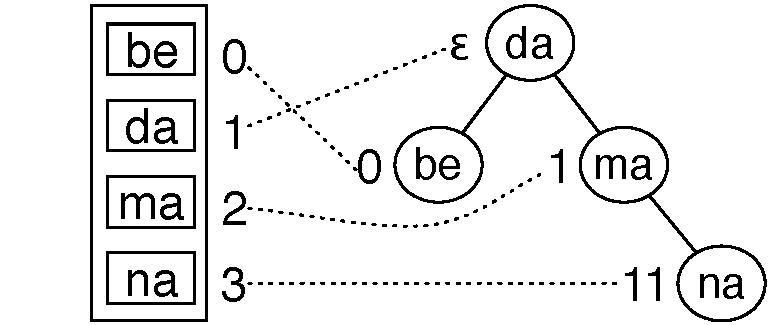
\includegraphics[scale=.32]{images/restruct1.pdf}
\end{wrapfigure}
The lens $\ell\in I\lens I'$ does not know anything about the intended
application; it has a trivial complement $\Unit$ and
merely maintains the constraint that the list shape and the tree shape
have the same number of positions. It has some freedom how it
translates list edits; e.g., it might add and remove tree nodes at the
left.

\ifdissertation
    \begin{wrapfigure}{r}{2in}
    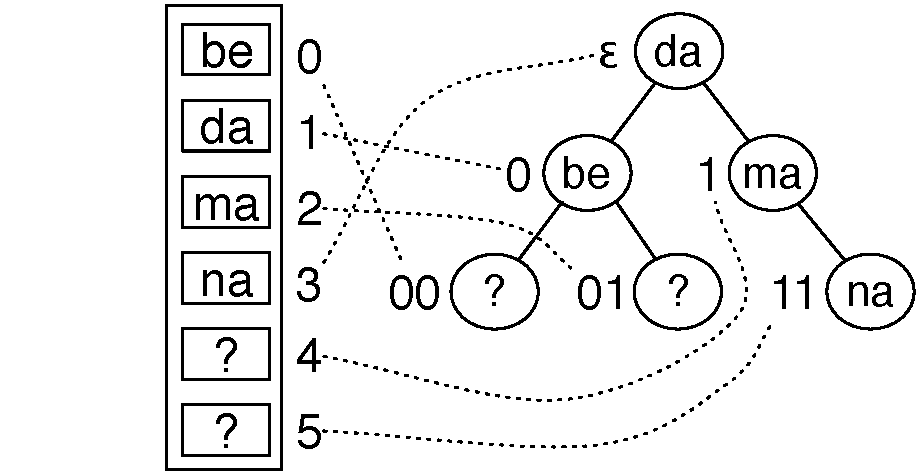
\includegraphics[scale=.32]{images/restruct2.pdf}
    \end{wrapfigure}
    The family of bijections $f_{i,c,i'}$ models the in-order correspondence;
\else
    The family of bijections $f_{i,c,i'}$ models the in-order
    \begin{wrapfigure}[9]{r}{1.3in}
    \hspace*{-4.3em}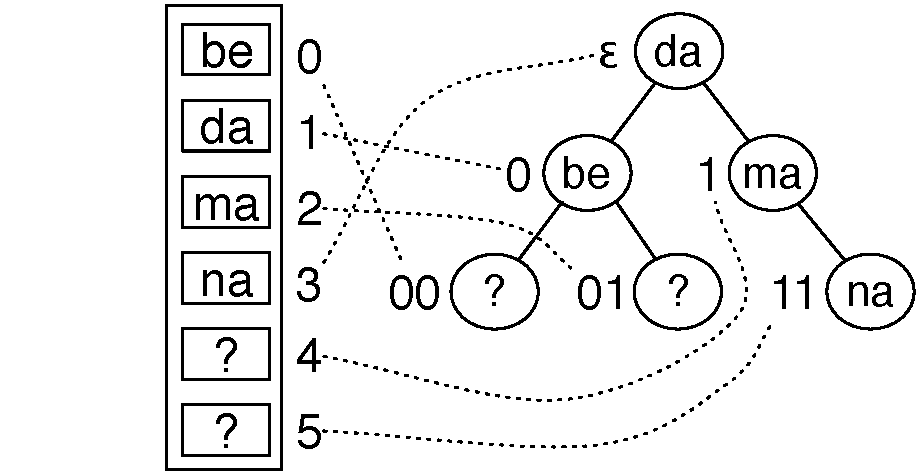
\includegraphics[scale=.32]{images/restruct2.pdf}
    \end{wrapfigure}
    correspondence;
\fi
thus, for example if $i=4$ and $i'=\{\NIL, \blist0\elist, \blist1\elist,
\blist1\mlist1\elist\}$ the bijection
would be as shown above. (For illustration we also indicate possible
$X$-contents of the positions.)
%
Formally, we have $f_{i,c,i'} = \{(0,\blist0\elist), (1,\NIL),
(2,\blist1\elist), (3,\blist1\mlist1\elist)\}$.

Now suppose that $\di\, i = i+2$ and that $\di'$ (the result of $\di$ propagated
through $\ell$) installs two children at the leftmost node. 
%
In our in-order application we then have $f_{\di\, i, c', \di'\, i'} =
\{(0,\blist0\mlist0\elist)$, $(1,\blist0\elist)$,
$(2,\blist0\mlist1\elist)$, $(3,\NIL)$, $(4,\blist1\elist)$,
$(5,\blist1\mlist1\elist)\}$ and
after applying both $\mlinsert(\di)$ and $\mlinsert(\di')$ we are in the
as-yet-inconsistent situation depicted above.
%% \begin{verbatim}
%% 0:be              eps:da
%% 1:da            /       \
%% 2:ma           0:be     1:ma
%% 3:na         /   \          \
%% 4:?        00:?  01:?        11:na
%% 5:?

%% Include the f-links, this time they go wild, eg 0 ----- 00 
%% \end{verbatim}

\ifdissertation\begin{wrapfigure}{r}{2in}
\else          \begin{wrapfigure}[9]{r}{1.3in}\hspace*{-4.3em}
\fi
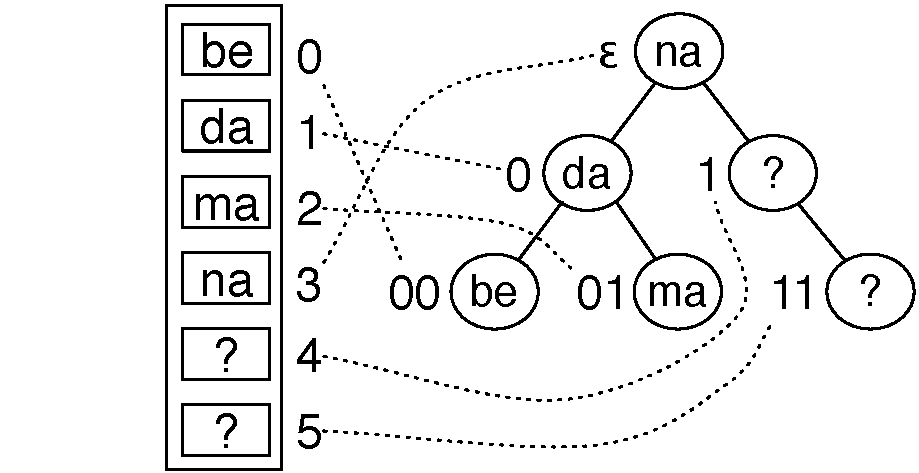
\includegraphics[scale=.32]{images/restruct3.pdf}
\end{wrapfigure}
Since the newly inserted elements in the list come at the end, we can
restore consistency by moving the newly inserted tree elements to positions
that come at the end of the in-order walk. This can be done essentially
automatically just using the in-order walk position bijections: to decide
where a position $p$ in the old tree should reappear in the new tree, we can
simply follow the position through its journey of being flattened and
unflattened using $f_{i,c,i'}$ and $f_{\di\;i,c',\di'\;i'}^{-1}$,
respectively. Thus to restore consistency we apply $\mlrearrange(\ONE,f_\mli)$ where
$f_\mli(i')=\{(\blist0\mlist0\elist,\blist0\elist)$, $(\blist0\elist,\NIL)$,
$(\blist0\mlist1\elist,\blist1\elist)$, $(\NIL,\blist1\mlist1\elist)$,
$(\blist1\elist,\blist0\mlist0\elist)$,
$(\blist1\mlist1\elist,\blist0\mlist1\elist)\}$. We could also have chosen
$f_\mli(i')= \{\dots, (\blist1\elist,\blist0\mlist1\elist)$,
$(\blist1\mlist1\elist,\blist0\mlist1\elist)\}$; since in any case the new
positions are uninitialized, this free choice has little impact.
Of course $f_\mli(i'')$ for $i''\neq i'$ is also
completely unconstrained. After applying $\mlrearrange(\ONE,f_\mli)$ we end up
with the desired consistent state.
%% \begin{verbatim}
%% 0:be              eps:na
%% 1:da            /       \
%% 2:ma          0:da     1:?
%% 3:na         /   \        \
%% 4:?        00:be  01:ma    11:?
%% 5:?
%% \end{verbatim}

\begin{figure}
% http://tex.stackexchange.com/q/121925/16779
\newtoggle{wide-equation}
\ifdissertation\settoggle{wide-equation}{true}\else\settoggle{wide-equation}{false}\fi
\newcommand{\wideeqbreak}{\iftoggle{wide-equation}{}{\\ &&}}
% \vspace*{-2.5ex}
\lensdef{w_restructuring}
{\infruleplain{T = \left<I,P,\live\right>\mbox{ a container type} \\
               T' = \left<I',P',\live'\right>\mbox{ a container type} \\
               \ell \in I \lens I'}
              {[T,T'](\ell) \in T(X) \lens T'(X)}}
 { C &=& \ell.K
  \\[.8ex]
  \missing &=& (\init_I,\ell.\missing,\init_{I'}) \\[.8ex]
  \colspan{K = \{ ((i,f),(i,c,i'),(i',f'))} \\
  \colspan{\qquad \;|\; (i,c,i')\in \ell.K \wedge \,\forall p{\in}\live'(i'). f(f_{i,c,i'}(p))=f'(p) \} } \\[1ex]
  \dputr\gen(\fail,x) &=& (\fail,x)\\
  \dputr\gen(\mlmod p\dx,(i,c,i')) &=& (\mlmod{f^{-1}_{i,c,i'}(p)}\dx, (i,c,i')) \\
  && \text{when }p\in\live(i)\\
  \dputr\gen(\mlinsert(\di),(i,c,i')) &=&
      (\mlrearrange(\ONE,f_\mli)\mlinsert(\di'), \wideeqbreak
      (\di\;i, c', \di'\;i'))\\
  \dputr\gen(\mldelete(\di),(i,c,i')) &=&
    (\mldelete(\di')\mlrearrange(\ONE,f_\mld), \wideeqbreak
    (\di\;i, c', \di'\;i'))\\
  \dputr\gen(\mlrearrange(\di,g),(i,c,i')) &=&
    (\mlrearrange(\di',f_\mlr), \wideeqbreak
    (\di\;i,c',\di'\;i'))\\[.8ex]
  && \text{see below for $f_\mli,f_\mld,f_\mlr$}\\
  \text{in the last three clauses:} && (\di',c')=\ell.\dputr(\di,c)\\
  \dputr\gen(\text{d}c,(i,c,i')) &=& \fail\text{ in all other cases}\\
  \dputl\gen(-,-) &=& \text{analogous}
  }
%
\makeatletter\refstepcounter{\@captype}\makeatother
\label{fig:restructuring-definition}
\vspace*{-3ex}
\begin{center}
{\bf Figure \ref{fig:restructuring-definition}:} Container restructuring lens
\end{center}
\vspace*{-3ex}
%  \caption{A lens for restructuring containers.}
\end{figure}

With this intuition in hand, we are ready to see the details of the
restructuring lens. As discussed above, we must have containers $T$ and
$T'$, an edit lens $\ell$ between their shapes, and a family of bijections
between live sets. We also require that $\ell$ maps insertions to
insertions, deletions to deletions, and rearrangements to rearrangements.
(This is well-defined on equivalence classes of lenses.)
Given these data, we define the restructuring lens in
Figure~\ref{fig:restructuring-definition}, with a few supplementary
definitions below.
%
The additional families of bijections $f_\mli, f_\mld, f_\mlr$ must be chosen in such a
way that the container edits in which they appear are well-formed
(this is possible since $\di'$ is an insertion, deletion, or
restructuring as appropriate) and such that the following three constraints are
satisfied: in each case $i,i'$, etc.,  refer to the current values from above and $p\in \live'(\di'\ i')$ is an arbitrary position. 
\begin{align*}
f_\mli(\di'\ i')(p) &=
\begin{array}[t]{@{}l}
f^{-1}_{i,c,i'}(f_{\di\ i,c',\di'\ i'}(p))\\ 
\quad \text{ when $f_{\di\ i,c',\di'\ i'}(p)\in\live(i)$}
\end{array}\\
f_\mld(i')(p) &= f^{-1}_{i,c,i'}(f_{\di\ i,c',\di'\ i'}(p))\\
f_\mlr(i')(p) &= f_{i,c,i'}^{-1}(g(i)(f_{\di\ i,c',\di'\ i'}(p)))
\end{align*}

These conditions do not completely determine $f_\mli$, $f_\mld$, and $f_\mlr$. In
each case, these families are completely unconstrained on shapes other than
$\di'\;i'$. The propagated edits are supposed to be applied to a container
of the current shape $i'$, so the arbitrary decisions about other shapes do
not really matter;
nevertheless it would be nice if we could be a bit more uniform. This
is indeed possible in the case where $\ell$ is an isomorphism lens, but we
refrain from formulating details.
% TODO: understand this sentence well enough to decide whether to formulate
% some details here-ish

As discussed in the example above, the bijection $f_\mli$ contains a little
more choice, namely the behavior on the $T'$ positions in $f_{\di\
i,c',\di'\ i'}^{-1}(\live(\di\ i)\setminus\live(i))$. Fortunately, they all
contain $\init_X$ so that the choice does not affect the resulting
state after application of the edit, and the alignment is decided not by
$f_\mli$ but by the family of bijections $f_{i,c',i'}$ that parameterize the
lens.

\iffull
\begin{theorem}
The restructuring lens is indeed a lens.
\end{theorem}
\begin{pf}
  As the edit monoid is free, we only need to show that successful
  edits to consistent states get transported to successful edits
  resulting in consistent states. Thus suppose that
  $(i,c,i')\in\ell.K$ and $f(f_{i,c,i'}(p))=f'(p)$ holds for all
  $p\in\live'(i')$ so that $((i,f),(i,c,i'),(i',f'))$ are consistent. We
  will show below that $\dputr$ is correct; the proof about $\dputl$ is very
  similar. In the cases below where there is an edit named $\di$, we will
  write $(\di',c')=\ell.\dputr(\di,c)$ and abbreviate the bijections
  $f_{i,c,i'}$ and $f_{\di\;i,c',\di'\;i'}$ to $f_{pre}$ and $f_{post}$,
  respectively.

  Case $\fail$ is obvious. 

  Case $\mlmod p\dx$: the complement does not change and the edit
  $\dx$ is applied to the same elements.

  Case $\mlins \di$. The resulting new repository states are $(\di\;i,f_1)$
  and $(\di'\;i', f_1')$:
  \begin{align*}
    f_1(p)&=\text{if }p\in\live(i)\text{ then }f(p)\text{ else }\init_X\\
    f_1'(p)&=\text{if }f_\mli(\di'\;i')(p)\in\live(i')\text{ then }f'(f_\mli(\di'\;i')(p))\text{ else }\init_X
  \end{align*}
Also, the bijection $f_\mli(\di'\ i')\in\live'(\di'\ i')\simeq \live'(\di'\ i')$ satisfies
\[
f_{post}(p)\in\live(i)\Rightarrow f_\mli(\di'\ i')(p)= f^{-1}_{pre}(f_{post}(p)).
\]
This assumption lets us conclude that $f_{post}(p) \in \live(i)$ if and only
if $f_\mli(\di'\;i')(p) \in \live'(i')$. In the forward direction, we argue:
\begin{align*}
    f_{post}(p) &\in \live(i) &&\mbox{assumption} \\
    f_{pre}^{-1}(f_{post}(p)) &\in \live'(i') &&f_{pre} \in \live(i) \simeq
    \live'(i') \\
    f_\mli(\di'\;i')(p) &\in \live'(i') &&\mbox{assumed condition of }f_\mli
\end{align*}
In the backward direction, define $q=f_\mli(\di'\;i')(p)$. Then:
\begin{align*}
    f_\mli(\di'\;i')(p) &\in \live'(i') &&\mbox{assumption} \\
    q &\in \live'(i') &&\mbox{definition of }q \\
    f_{pre}(q) &\in \live(i) &&f_{pre} \in \live(i) \simeq \live'(i') \\
    f_{post}(f_{post}^{-1}(f_{pre}(q))) &\in \live(i) &&f_{post}\mbox{ is a bijection} \\
    f_{pre}^{-1}(f_{post}(f_{post}^{-1}(f_{pre}(q)))) &= q
        &&f_{post}\mbox{ and }f_{pre}\mbox{ are bijections} \\
    f_\mli(\di'\;i')(f_{post}^{-1}(f_{pre}(q))) &= q
        &&\mbox{assumed condition of }f_\mli \\
    f_{post}^{-1}(f_{pre}(q)) &= p
        &&f_\mli(\di'\;i')\mbox{ is a bijection and} \\
       &&&\mbox{definition of }q \\
    f_{post}(p) &\in \live(i) &&f_{pre}(q)\in\live(i)
\end{align*}

To conclude the case, we must show that arbitrary $p \in \live'(\di'\;i')$
have $f_1'(p)=f_1(f_{post}(p))$. We consider two cases: either $f_{post}(p)
\in \live(i)$ or not. If so then $f_1(f_{post}(p))=$ $f(f_{post}(p)) = $
$f'(f_{pre}^{-1}(f_{post}(p)))= $ $f_1'(p)$ where the first equation uses
the above characterization of $f_1$; the second one uses consistency of $f$
and $f'$, and the third one uses the characterizations of $f_1'$ and $f_\mli$
(noting that $f_{post}(p) \in \live(i)$ implies $f_\mli(\di'\;i')(p) \in
\live'(i')$). In the other case, $f_{post}(p) \notin \live(i)$, so
$f_\mli(\di'\;i')(p) \notin \live'(i')$. Then $f_1'(p)=\init_X$, but
$f_1(f_{post}(p))=\init_X$, too, by the characterization of $f_1$.

  Case $\mldel \di$. Ignoring domain restrictions, the new repository states
  are $(\di\;i,f)$ and $(\di'\;i',f_\mld(i');f')$. For these to be consistent,
  we must show that $f(f_{post}(p)) = f'(f_\mld(i')(p))$ whenever $p \in
  \live'(\di'\;i')$. Since $\di$ is a deletion, we know $\di\;i \subset i$,
  so that $f_{post} \in \live(\di\;i) \simeq \live'(\di'\;i')$ implies
  $f_{post}(p) \in \live(i)$. Hence we can equate:
  \begin{align*}
      f(f_{post}(p)) &= f'(f_{pre}^{-1}(f_{post}(p)))
          &&\mbox{consistency of }f\mbox{ and }f'\\
      &= f'(f_\mld(i')(p)) &&\mbox{assumed condition of }f_\mld
  \end{align*}

  Case $\mlrearrange(\di,g)$. The new repository states that we must show
  are consistent are $(\di\;i,g(i);f)$ and $(\di'\;i',f_\mlr(i');f')$. Consider
  arbitrary $p \in \live'(\di'\;i')$. Since $f_{post};g(i) \in
  \live'(\di'\;i') \simeq \live(i)$, we know $g(i)(f_{post}(p)) \in
  \live(i)$; this justifies the first equation below.
    \begin{align*}
        f(g(i)(f_{post}(p))) &= f'(f_{pre}^{-1}(g(i)(f_{post}(p))))
            &&\mbox{consistency of }f\mbox{ and }f' \\
        &= f'(f_\mlr(i')(p))
            &&\mbox{condition of }f_\mlr
    \end{align*}
\vskip -1.8\baselineskip
\end{pf}
\fi

\iffull Using the container lens combinators, the
partition lens and
lens mediating between ``built-in'' lists and ``list containers'' we
can then plumb together a variety of useful lenses, e.g.\ one that
partitions the entries of an $X+Y$ labeled tree into $\inl$s and
$\inr$s and then presents the two resulting containers again as trees
over $X$ and $Y$. If one wants one can then use a mapping lens to
change the representation of the $Y$'s in some way.
\fi

\sect{Adding Monoid Laws}
\label{sec:monoid-laws}

The edit languages accompanying the constructions in the previous two
sections were all freely generated.  This was a good place to begin as it
is relatively easy to understand, but, as discussed in \S
\ref{sec:semantics}, there are good reasons for investigating richer
languages.  This section takes a first step in this direction by showing how
to equip the product and sum combinators with more interesting edits. 

Given modules $X$ and $Y$, there is a standard definition of {\em module
  product} 
motivated by the intuition that an edit to an $|X| \times |Y|$ value is a
pair of an edit to the $|X|$ part and an edit to the $|Y|$ part. The monoid
multiplication goes pointwise, and one can define an edit application that
goes pointwise as well.
\[
\begin{array}{@{}c@{}}
X \otimes Y = \left<|X| \times |Y|,(\init_X,\init_Y),\partial X \otimes
\partial Y,\odot_{X \otimes Y}\right> \\[.6ex]
\ONE_{M \otimes N} = (\ONE_M,\ONE_N) \\[.6ex]
(m,n)\cdot_{M \otimes N}(m',n') = (m\,m', n\,n')\\[.6ex]
(\dx,\dy)\odot_{X \otimes Y}(x,y) = (\dx\,x,\dy\,y)
\end{array}
\]

\iffull
\begin{lemma}
    These definitions give rise to a module---that is, $\cdot_{M \otimes N}$
    is associative with identity $\ONE_{M \otimes N}$ and $\odot_{X \otimes Y}$
    satisfies the monoid action laws.
\end{lemma}
\begin{proof}
    To show that $\cdot_{M \otimes N}$ is associative, using the fact that
    $\cdot_M$ and $\cdot_N$ are associative:
    \begin{align*}
        v_1 \cdot (v_2 \cdot v_3)
            &= (m_1,n_1) \cdot ((m_2,n_2) \cdot (m_3,n_3)) \\
            &= (m_1,n_1) \cdot (m_2 \cdot m_3,n_2 \cdot n_3) \\
            &= (m_1\cdot(m_2 \cdot m_3),n_1\cdot(n_2 \cdot n_3)) \\
            &= ((m_1 \cdot m_2) \cdot m_3,(n_1 \cdot n_2) \cdot n_3) \\
            &= (m_1 \cdot m_2, n_1 \cdot n_2)\cdot(m_3,n_3) \\
            &= ((m_1,n_1) \cdot (m_2,n_2)) \cdot (m_3,n_3) \\
            &= (v_1 \cdot v_2) \cdot v_3
    \end{align*}
    To show that $\ONE_{M \otimes N}$ is an identity for $\cdot_{M \otimes
    N}$, assuming $\ONE_M$ and $\ONE_N$ are the respective identities for
    $\cdot_M$ and $\cdot_N$:
    \begin{align*}
        (\ONE,\ONE)\cdot(m,n)
            &= (\ONE \cdot m,\ONE \cdot n) \\
            &= (m,n) \\
            &= (m \cdot \ONE,n \cdot \ONE) \\
            &= (m,n) \cdot (\ONE, \ONE)
    \end{align*}
    To show the monoid action laws are satisfied by $\odot_{M \otimes N}$,
    assuming these laws are satisfied by $\odot_M$ and $\odot_N$:
    \begin{align*}
        (\ONE,\ONE) \odot (x,y)
            &= (\ONE \odot x, \ONE \odot y) \\
            &= (x,y) \\
        ((m,n)\cdot(m',n'))\odot(x,y)
            &= (m \cdot m',n \cdot n')\odot(x,y) \\
            &= ((m \cdot m') \odot x,(n \cdot n') \odot y) \\
            &= (m \odot m' \odot x,n \odot n' \odot y) \\
            &= (m,n) \odot (m' \odot x,n' \odot y) \\
            &= (m,n) \odot (m',n') \odot (x,y)
    \end{align*}
\end{proof}
\fi

One might wonder whether the standard definition has any connection to the
definition we give earlier. One way to bridge the gap is to add equational
laws to the free monoid\footnote{To make this formal, treat the
equations as a relation between words in the free monoid; take the
reflexive, symmetric, transitive, congruence closure of this relation; and
quotient by the resulting equivalence relation.}. The equations below demand
that $\ml{left}$ and $\ml{right}$ be monoid homomorphisms, and that they
commute:
\begin{align*}
    \blist\mlleft\ONE\elist &= \NIL \\
    \blist\mlleft\dx\mlist\mlleft{\dx'}\elist &= \blist\mlleft{\dx\;\dx'}\elist \\
    \blist\mlright\ONE\elist &= \NIL \\
    \blist\mlright\dy\mlist\mlright{\dy'}\elist &= \blist\mlright{\dy\;\dy'}\elist \\
    \blist\mlleft\dx\mlist\mlright\dy\elist &= \blist\mlright\dy\mlist\mlleft\dx\elist
\end{align*}
It is not hard to show that the free monoid subject to the above
equations is isomorphic to the natural monoid product.

However, it is not obvious that the definitions relying on the free monoid
product remain well defined after imposing the above equations. In
particular, we must check that any monoid homomorphisms we defined respect
these laws. For homomorphisms $f$ specified via specification
of $f\gen$, it is enough to prove that, for each equational law $g=g'$, the
specification respects the law---i.e., $f(g)=f(g')$.

For example, to check that we can create a well-defined tensor product
module that includes the above equations, we must show that $\odot\gen$
respects the equations. For the commutativity equation, we must show 
\[\mlleft\dx\odot\gen\mlright\dy\odot\gen(x,y) =
\mlright\dy\odot\gen\mlleft\dx\odot\gen(x,y).\]
Simple calculation shows that both sides are equal to $(\dx\;x,\dy\;y)$, so
this law is respected; the rest follow similar lines.

Most importantly, we must check that the $\dputr$ and $\dputl$ functions are
still monoid homomorphisms; indeed, this check
makes these equations interesting as a {\em specification}: 
in addition to the usual round-tripping laws we expect of
state-based lenses, each non-trivial equation in a monoid presentation
represents a behavioral limitation on lenses operating on that monoid.
Take again the commutativity law:
\[\mlleft\dx\;\mlright\dy = \mlright\dy\;\mlleft\dx\]
The force of this law is that lenses operating on a monoid including this
equation must ignore the interleaving of $\ml{left}$ and $\ml{right}$ edits:
those two edits are treated independently by the lens.

\begin{lemma}
    Suppose $k$ and $\ell$ are lenses. For each of the equations above, if
    that equation is in force in the modules on both sides of the
    $k\otimes\ell$ lens, then the $\dputr$ and $\dputl$ functions defined
    above for this lens respect that equation.
\end{lemma}
\begin{proof}
We will show that $\dputr$ treats $\ml{left}$ as a monoid homomorphism and
lets $\ml{left}$ and $\ml{right}$ commute; the proofs that $\dputr$ treats
$\ml{right}$ as a monoid homomorphism and that $\dputl\gen$ respects all these
laws are similar.

To show that $\dputr$ respects the law $\blist\mlleft\ONE\elist=\NIL$:
\begin{align}
    \dputr(\blist\mlleft\ONE\elist,(c_k,c_\ell))
        ={}& \mllet (\dz,c_k')=k.\dputr(\ONE,c_k)\mline \nonumber\\
           & (\blist\mlleft\dz\elist,(c_k',c_\ell)) \nonumber\\
        ={}& (\blist\mlleft\ONE\elist,(c_k,c_\ell)) \label{eq:klens} \\
        ={}& (\NIL,(c_k,c_\ell)) \label{eq:law} \\
        ={}& \dputr(\NIL,(c_k,c_\ell)) \label{eq:one2}
\end{align}
Equation~\ref{eq:klens} follows because $k$ is a lens and hence $k.\dputr$
is a stateful monoid homomorphism. Equation~\ref{eq:law} follows by
assumption, and equation~\ref{eq:one2} follows by definition of $\dputr$.

Next we will show that $\dputr$ respects the law
$\blist\mlleft\dx\mlist\mlleft{\dx'}\elist=\blist\mlleft{\dx\dx'}\elist$. It
will be convenient to name a few things. Pick a state $c_k$ and define:
\begin{align*}
    (\dy',c_k') &= k.\dputr(\dx',c_k) \\
    (\dy,c_k'') &= k.\dputr(\dx,c_k')
\end{align*}
Since $k$ is a lens and hence in particular $k.\dputr$ is a stateful monoid
homomorphism, we can conclude that:
\[k.\dputr(\dx\dx',c_k)=(\dy\dy',c_k'')\]
We may now compute:
\[\begin{array}{l}
    \dputr(\blist\mlleft\dx\mlist\mlleft{\dx'}\elist,(c_k,c_\ell)) \\
    \qquad=
        \mllet (\dy',(c_k',c_\ell')) = \dputr\gen(\mlleft{\dx'},(c_k,c_\ell)) \mline \\
    \qquad{\phantom{={}}}
        \mllet (\dy'',(c_k'',c_\ell'')) = \dputr\gen(\mlleft\dx,(c_k',c_\ell')) \mline \\
    \qquad{\phantom{={}}}
        (\blist\dy''\mlist\dy'\elist,(c_k'',c_\ell'')) \\
    \qquad=
        \mllet (\dy'',(c_k'',c_\ell'')) = \dputr\gen(\mlleft\dx,(c_k',c_\ell)) \mline \\
    \qquad{\phantom{={}}}
        (\blist\dy''\mlist\mlleft{\dy'}\elist,(c_k'',c_\ell'')) \\
    \qquad=
        (\blist\mlleft\dy\mlist\mlleft{\dy'}\elist,(c_k'',c_\ell)) \\
    \qquad=
        (\blist\mlleft{\dy\dy'}\elist,(c_k'',c_\ell)) \\
    \qquad=
        \dputr\gen(\mlleft{\dx\dx'},(c_k,c_\ell)) \\
    \qquad=
        \dputr(\blist\mlleft{\dx\dx'}\elist,(c_k,c_\ell))
\end{array}\]

\ifdissertation
The final equation to preserve is
\else
Finally, we show that $\dputr$ respects the law
\fi
$\blist\mlleft\dx\mlist\mlright\dy\elist=\blist\mlright\dy\mlist\mlleft\dx\elist$.
As before, we choose a $c_k$ and $c_\ell$ and name a few intermediate
computations:
\begin{align*}
    (\dx',c_k') &= k.\dputr(\dx,c_k) \\
    (\dy',c_\ell') &= \ell.\dputr(\dy,c_\ell)
\end{align*}
Now we may compute:
\[\begin{array}{l}
\dputr(\blist\mlleft\dx\mlist\mlright\dy\elist,(c_k,c_\ell)) \\
    \qquad=
        \mllet (\dy',(c_k',c_\ell')) = \dputr\gen(\mlright\dy,(c_k,c_\ell)) \mline \\
    \qquad{\phantom{={}}}
        \mllet (\dx',(c_k'',c_\ell'')) = \dputr\gen(\mlleft\dx,(c_k',c_\ell')) \mline \\
    \qquad{\phantom{={}}}
        (\blist\dx'\mlist\dy'\elist,(c_k'',c_\ell'')) \\
    \qquad=
        \mllet (\dx',(c_k'',c_\ell'')) = \dputr\gen(\mlleft\dx,(c_k,c_\ell')) \mline \\
    \qquad{\phantom{={}}}
        (\blist\dx'\mlist\mlright{\dy'}\elist,(c_k'',c_\ell'')) \\
    \qquad=
        (\blist\mlleft{\dx'}\mlist\mlright{\dy'}\elist,(c_k',c_\ell')) \\
    \qquad=
        (\blist\mlright{\dy'}\mlist\mlleft{\dx'}\elist,(c_k',c_\ell')) \\
    \qquad=
        \dputr(\blist\mlright\dy\mlist\mlleft\dx\elist,(c_k,c_\ell))
\end{array}\]
The final line follows from the previous one by an argument almost identical
(but reversed) to the argument showing that the second-to-last line follows
from the first.
\end{proof}

Adding the first four equations lets us create a projection lens
out of smaller parts by observing that there are some new isomorphisms
available.
\iffull

\begin{defn}[Projection lenses]
\fi
Let $f$ and $g$ be the obvious isomorphisms connecting $X \otimes \Unit$ to
$X$ and $\Unit \otimes Y$ to $Y$.%
%
\iffull
\footnote{%
  \ifdissertation
  Unlike the analogous state-based lenses from Chapter~\ref{chap:complement},
  \else
  Readers familiar with earlier work on symmetric state-based
  lenses~\cite{HofmannPierceWagner10} may observe that, unlike the analogous
  state-based lenses,
  \fi these projections are \emph{not} parameterized by an
  element of the set that is being projected away. Never fear: this element
  is still available, as the $\init$ value of the appropriate module.
  }
\fi
%
\iffull
    \begin{align*}
        \pi_1 &= (\id_X \otimes \const_Y);\bij_f \\
        \pi_2 &= (\const_X \otimes \id_Y);\bij_g
    \end{align*}
\else
{} We can then define $\pi_1 = (\id_X \otimes \const_Y);\bij_f$ and $\pi_2 =
(\const_X \otimes \id_Y);\bij_g$. Thus, $\pi_1$ first throws away any
information in the right-hand part of a tuple with $\const_Y$, then
collapses the (now degenerate) tuple with $f$.
\fi
\iffull \end{defn} \fi

We conjecture that these additional laws introduce enough isomorphisms that
the tensor product gives rise to a symmetric monoidal category---that is,
that tuples may be reordered and reassociated freely, provided the lens
program acting on them is reordered and reassociated accordingly---but we
have not explored this possibility fully.

\iflater
\finish{To define a more useful diagonal in this setting, we could
  consider enriching the monoid structure with a $\mathit{merge}$
  operation...}
\fi

We can perform a similar process for sum edits. We add the following
equations:
\begin{align*}
    \blist\mlswitch_{jk}(m)\mlist\mlswitch_{ij}(m')\elist
        &= \blist\mlswitch_{ik}(m)\elist \\
    \blist\mlswitch_{ij}(m)\mlist\mlstay_i(m')\elist
        &= \blist\mlswitch_{ij}(m)\elist \\
    \blist\mlstay_j(m)\mlist\mlswitch_{ij}(m')\elist
        &= \blist\mlswitch_{ij}(mm')\elist \\
    \blist\mlstay_i(m)\mlist\mlstay_i(m')\elist
        &= \blist\mlstay_i(mm')\elist \\
    \blist d\mlist d'\elist
        &= \blist\fail\elist \qquad \mbox{in all other cases}
\end{align*}
This explains why we did not originally choose to have just two combinators,
$\mlswitch_L$ and $\mlswitch_R$, which would be interpreted as ``switch to
the left (respectively, right) side and reinitialize, no matter which side
we are currently on\dotquote The idea of the above equations is that they allow
us to collapse any sequence of edits down into a single one; if we only
allowed ourselves $\mlswitch_L$ and $\mlswitch_R$ forms, this would not be
possible. In particular, we need to represent the fact that a $\mlstay_L$
edit followed by a $\mlswitch_i$ edit fails when applied to a value tagged
with $\mlinrx$.

As with products, we must check that the remaining
definitions are well-formed.  \iffull\else In particular, it can be shown that,
in the module defined above for sums, $\odot\gen$ respects the above
equations, and that, if $k$ and $\ell$ are lenses, then
$(k\oplus\ell).\dputr\gen$ and $(k\oplus\ell).\dputl\gen$ respect the above
equations.  \fi

% TODO: \ml{inl} -> \mlinlx ?
\iffull
\begin{lemma}
    In the module defined above for sums, $\odot$ respects the above
    equations.
\end{lemma}
\begin{proof}
    We will give proofs for the first four equations with $i$, $j$, and $k$
    instantiated to $L$ (proofs for other instantiations are nearly
    identical). The final equation is respected because every pair of atomic
    edits not listed in the first four equations results in an edit that
    cannot be successfully applied to any value (just like the $\fail$ edit
    itself).

    For each of the four equations (instantiated to $L$ everywhere) $e=e'$,
    both $e\odot\mlinr y$ and $e'\odot\mlinr y$ are undefined, so we focus
    on $e\odot\mlinl x$ and $e'\odot\mlinl x$.
    \begin{align*}
        \blist\mlswitchll m\mlist\mlswitchll{m'}\elist \odot \mlinl x
            &= \blist\mlswitchll m\elist\odot \mlinl{m'\odot \init} \\
            &= \mlinl{m \odot \init} \\
            &= \blist\mlswitchll{m}\elist \odot \mlinl x \\
        \blist\mlswitchll m\mlist\mlstayl{m'}\elist \odot \mlinl x
            &= \blist\mlswitchll m\elist \odot \mlinl{m'\odot x} \\
            &= \mlinl{m \odot \init} \\
            &= \blist\mlswitchll m\elist \odot \mlinl x \\
        \blist\mlstayl m\mlist\mlswitchll{m'}\elist \odot \mlinl x
            &= \blist\mlstayl m\elist \odot \mlinl{m' \odot \init} \\
            &= \mlinl{m \odot m' \odot \init} \\
            &= \mlinl{mm' \odot \init} \\
            &= \blist\mlswitchll{mm'}\elist \odot \mlinl x \\
        \blist\mlstayl m\mlist\mlstayl{m'}\elist \odot \mlinl x
            &= \blist\mlstayl m\elist \odot \mlinl{m' \odot x} \\
            &= \mlinl{m \odot m' \odot x} \\
            &= \mlinl{mm' \odot x} \\
            &= \blist\mlstayl{mm'}\elist \odot \mlinl x
    \end{align*}
    \vskip -5ex
\end{proof}

\begin{lemma}
    If $k$ and $\ell$ are lenses, then $(k\oplus\ell).\dputr\gen$ and
    $(k\oplus\ell).\dputl\gen$ respect the above equations.
\end{lemma}
\fi

\iffull
\begin{pf}
    We will show only that $\dputr\gen$ respects the equations; the argument
    for $\dputl\gen$ is similar. Choose arbitrary sum edits $e_1,e_2$ and
    initial complement $c_0 \in C$ and define:
    \begin{align*}
        e_{12} &= e_2e_1 \\
        (f_1,c_1) &= \dputr(e_1,c_0) \\
        (f_2,c_2) &= \dputr(e_2,c_1) \\
        (f_{12},c_{12}) &= \dputr(e_2e_1,c_0)
    \end{align*}
    We must show that $f_{12}=f_2f_1$ and $c_{12}=c_2$. We will go by case
    analysis on $e_1$ and $e_2$; however we can first rule out a few broad
    categories of such cases. When
    $\dputr(e_1,c)=(\fail,\mlfailed)$ fails, there is very little to prove;
    we know that $\dputr(e_2,\mlfailed)=(f_2,\mlfailed)$ for some $f_2$, and
    hence that $f_2f_1=\fail$. Furthermore, it is not hard to see by
    inspecting the cases where $\dputr(e_1,c)$ fails that $\dputr(e_{12},c)$
    will also fail for any $e_2$. Hence $f_{12}=\fail=f_2f_1$ and
    $c_{12}=\mlfailed=c_2$. Similarly, when $e_2$ results in a failure, any
    combined edit $e_{12}$ will also result in failure.  As a final broad
    category, when the lens has already failed (that is, when
    $c_0=\mlfailed$), we observe that the lens preserves the ``constructor''
    of the edit. Since the monoid multiplication inspects only the
    constructor, the required equation $f_2f_1=f_{12}$ will hold, and we
    will have $c_{12}=\mlfailed=c_2$.

    In the following, we therefore assume that no failure occurs.
    A few definitions will be convenient: \finish{the $s$ definition could
    have been used in the definition of the lens.} 
    \begin{align*}
        s(L,\dx)     &= k.\dputr(\dx,k.\missing) &
        t(L,x)       &= \mlinl x &
        u(\mlinl x)  &= L \\
        s(R,\dx)     &= \ell.\dputr(\dx,\ell.\missing) &
        t(R,y)       &= \mlinr y &
        u(\mlinr y)  &= R \\
        &&&&
        u(\mlfailed) &= \mlfailed
    \end{align*}
    The cases now proceed as follows:
    \begin{trivlist}

\nextcase{$e_1=\mlswitch_{hi}(\dx'),e_2=\mlswitch_{ij}(\dx)$} We have
            $e_2e_1=\mlswitch_{hj}(\dx)$. Since we consider only non-failing
            cases, we know $u(c_0)=h$---that is to say, the complement and the
            edit are consistent, and
            we are translating a ``sensible'' edit. We know two
            things: first, $f_1 = \mlswitch_{hi}(\dy')$ for some $\dy'$, and
            second, $u(c_1)=i$. From there, we can define
            $(\dy,c) = s(j,\dx)$, 
            so that
            $(f_2f_1,c_2) = (\mlswitch_{hj}(\dy),t(j,c))$.
            Moreover, simple calculation (again observing that $u(c_0)=h$
            and hence that $e_{12}$ is a sensible edit to apply, according
            to the complement) shows that also
            $(f_{12},c_{12}) = (\mlswitch_{hj}(\dy),t(j,c))$,
            which is equal to the previous tuple, as desired.

\nextcase{$e_1=\mlstay_i(\dx),e_2=\mlswitch_{ij}(\dx')$} Since we know no
            failure occurs, we must have $u(c_0)=i$.
            Therefore, $e_2$ is a sensible edit to apply, and so
            \[\dputr(e_2,c_0) = (\mlswitch_{ij}(\dy'),t(j,c))\]
            where $(\dy',c)=s(j,\dx')$. Furthermore, $e_1$ is a sensible
            edit to apply, so we know $u(c_1)=i$, and hence that $(f_2,c_2)
            = (\mlswitch_{ij}(\dy'),t(j,c))$. Furthermore, since $f_1 =
            \mlstay_i(\dy)$ for some $\dy$, we know $f_2f_1=f_2$. But since
            $e_{12}=e_2$,
            \begin{align*}
                (f_{12},c_{12}) &= \dputr(e_{12},c_0) \\
                &= \dputr(e_2,c_0) \\
                &= \dputr(e_2,c_1) \\
                &= (f_2,c_2) \\
                &= (f_2f_1,c_2)
            \end{align*}
            as desired.

\nextcase{$e_1=\mlswitch_{ij}(\dx'),e_2=\mlstay_j(\dx)$} Again, we observe
            that we must have $u(c_0)=i$. Therefore we simply appeal to the
            homomorphism laws
            for $k.\dputr$ (when $j=L$) or $\ell.\dputr$ (when $j=R$). For
            example, when $j=L$ and hence $c_0=\mlinl c$, we can define:
            \begin{align*}
                (\dy',c') &= k.\dputr(\dx',k.\missing) \\
                (\dy,c'') &= k.\dputr(\dx,c') \\
                (\dy'',c''') &= k.\dputr(\dx\dx',k.\missing)
            \end{align*}
            Then, by computation:
            \begin{align*}
                (f_1,c_1) &= (\mlswitch_{il}(\dy'),\mlinl{c'}) \\
                (f_2,c_2) &= (\mlstayl\dy,\mlinl{c''}) \\
                (f_{12},c_{12}) &= (\mlswitch_{il}(\dy''),\mlinl{c'''}) \\
                f_2f_1 &= \mlswitch_{il}(\dy\dy')
            \end{align*}
            Finally, appealing to $k.\dputr$'s homomorphism law, we conclude
            $\dy''=\dy\dy'$ and $c'''=c''$, and hence that
            $(f_2f_1,c_2)=(f_{12},c_{12})$.

\nextcase{$e_1=\mlstay_i(\dx'),e_2=\mlstay_i(\dx)$} Much like the
            previous case, since $u(c_0)=i$, we appeal directly to the
            homomorphism law for the underlying $\dputr$ operations; the
            only difference from the previous case is that we begin with a
            complement that may not be $k.\missing$ or $\ell.\missing$.
    \endofpf
    \end{trivlist}
\end{pf}
\fi%full

Unfortunately, the $\partition$ lens as given does {\em not} respect the
above equations.  It seems possible to enforce them by also imposing
equations on list edits that coalesce adjacent $\ml{reorder}$ operations. We
leave this to future work.

In a similar vein, we can impose equations on container edits---indeed, we
need them, since we would like lists to form a
special case of containers so that, possibly after
\emph{restructuring}, we can \emph{partition} and reassemble
containers, too. These equations would in particular allow us to
coalesce adjacent reorderings and to reorder insertions and
deletions with other edits so that insertions and deletions
always come first. This would also give rise to a compact normal
form of container edits. Again, we leave this to future work. 

\sect{From State-Based to Edit Lenses and Back} 
\label{stateb}

\ifcomplement
In \cite{HofmannPierceWagner10}, we introduced a
state-based framework for bidirectional transformations called
\emph{symmetric lenses}.  We refer to them here as \emph{state-based symmetric
  lenses}.
\fi
Recall from\symmlenses that a state-based symmetric lens $\ell$
between \emph{sets} $X$ and $Y$ comprises a set of complements $C$, a
distinguished element $\smissing \in C$, and two functions
\begin{eqnarray*}
    \putr &\in& X \times C \to Y \times C\\
    \putl &\in& Y \times C \to X \times C
\end{eqnarray*}
\ifdissertation
satisfying some round-tripping laws.
\else
satisfying the following round-tripping laws:
\infrule[PutRL]{\putr(x,c) = (y,c')}{\putl(y,c') = (x,c')}
\infrule[PutLR]{\putl(y,c) = (x,c')}{\putr(x,c') = (y,c')} 
Equivalence of state-based symmetric lenses is defined through the
existence of a simulating relation between the respective complement
sets that relates the $\smissing$ elements and is preserved by
$\putl,\putr$. A characterization in terms of ``dialogues'' is also given. 
%
State-based symmetric lenses modulo equivalence form a category (they
compose) and support a variety of constructions, in particular tensor
product, sum, lists, trees, and container types.

\fi
Now, for any set $X$ we have the monoid $O_X$ whose elements (edits)
are lists of overwriting elements of $X$ modulo the equality $xx=x$. An
action of $O_X$ on $X$ is defined by $\NIL x=x$ and $\blist x\mlist w\elist\;y=x$
where $x\in X, w\in X\LIST$. Note that this is well defined as
$x(xy)=x=xy$. If, in addition, we have a distinguished element $x\in
X$, we thus obtain a module denoted $X_x$ where $|X_x|=X$ and
$\init_X=x$ and $\DX_x = O_X$.

\iffull
We are now ready to give the definition of the lifting operation that turns
any symmetric, state-based lens between inhabited types into a symmetric
edit lens\footnote{The unique state-based lens between uninhabited types can
be lifted to the unique edit lens between degenerate modules.}.
\lensdef{editize}
{\infruleplain
    {\ell \in X \sslens Y \qquad x \in X\\
     \ell.\putr(x,\ell.\smissing) = (y,c_0)
    }
    {\D_x\ell \in X_x \lens Y_y}
}
{
    C &=& \ell.C \\
    \missing &=& c_0 \\
    K &=& \{(x,c,y) \mid \ell.\putr(x,c)=(y,c)\} \\
    \dputr\gen &=& \ell.\putr \\
    \dputl\gen &=& \ell.\putl
}
\else
Let  $\ell$ be  a state-based symmetric lens between $X$
and $Y$ along with element $x\in X$. Defining
$(y,c_0)=\ell.\putr(x,\ell.\smissing)$,
we then construct a symmetric edit lens $\D_x \ell$ between the
modules $X_x$ and $Y_y$ 
as follows: 
(1) $(\D_x\ell).C = \ell.C$;
(2) $(\D_x\ell).\missing = c_0$;
(3) $(\D_x\ell).\dputr\gen = \ell.\putr$;
(4) $(\D_x\ell).\dputl\gen = \ell.\putl$; and
(5) $(\D_x\ell).K = \{(x,c,y) \mid \ell.\putr(x,c)=(y,c)\}$.
\fi
$\D_x \ell$ is a symmetric edit lens and the passage from $\ell$
to $\D_x \ell$ is compatible with the equivalences on symmetric
lenses and symmetric edit lenses. The equations for $\dputr$ and $\dputl$
are well-defined because the round-trip law for symmetric lenses guarantees
that putting the same value twice in a row results in the same output both
times (hence if edits will be coalesced in $X_x$, they will be translated to
edits that get coalesced in $Y_y$),
and the consistency relation is likewise preserved because the roundtrip
laws for symmetric lenses guarantee that any given $\putr$ or $\putl$
results in a ``stable state''.

\iffull
\begin{theorem}
    If $k$ and $\ell$ are state-based lenses and $k\equiv\ell$, then
    $\D_xk\equiv\D_x\ell$.
\end{theorem}

\begin{proof}
Suppose $S$ is a witness that $k\equiv\ell$. Then we define
$\D_xS$ as follows:
\[\D_xS = \{(x,c_k,c_\ell,y) \mid (c_k,c_\ell) \in S
\land x \in X \land y \in Y\}\]

Let us write $(y_k,c_{0k})=k.\putr(x,k.\smissing)$ and
$(y_\ell,c_{0\ell})=\ell.\putr(x,\ell.\smissing)$. Since
$(k.\smissing,\ell.\smissing)\in S$, we know $y_k=y_\ell$ and
$(c_{0k},c_{0\ell})\in S$. The former equality tells us that at least the
two lenses have the same type---that is, $Y_{y_k}=Y_{y_\ell}$ as
modules---while the latter inclusion lets us observe that
\[(\init_{X_x},(\D_xk).\missing,(\D_x\ell).\missing,\init_{Y_y})=(x,k.\smissing,\ell.\smissing,y)\in\D_xS\]
where we abbreviate $y_k$ and $y_\ell$ by the name $y$.

It remains to show that $\D_xS$ is preserved by $\dputr$ and
$\dputl$ (definedness is not in question since the modules in question have
no partial edits); these arguments are very similar, so we focus on the one for
$\dputr$. We have $x_0 \in X,y_0 \in Y,(c_k,c_\ell) \in S,\dx \in X_x$. We
must show that computing $\dputr$ with these values produces values that
form a tuple in $\D_xS$. We proceed by induction on $\dx$.

In case $\dx=\NIL$, we are done: after computing $\dputr$, we still
have $x_0$, $y_0$, $c_k$, and $c_\ell$. Otherwise, $\dx = x_1\CONS\dx'$ and
the induction hypothesis tells us that if the two equations
\begin{align*}
(\D_xk).\dputr(\dx',c_k)&=(\dy_k,c_k')\\
(\D_x\ell).\dputr(\dx',c_\ell)&=(\dy_\ell,c_\ell')
\end{align*}
hold then $(c_k',c_\ell') \in S$ and $\dy_k=\dy_\ell$. We can then conclude
that if $k.\putr(x_1,c_k')=(y_k,c_k'')$ and
$\ell.\putr(x_1,c_\ell')=(y_\ell,c_\ell'')$ then $y_k=y_\ell$ and
$(c_k'',c_\ell'') \in S$ because $S$ is a witness that $k \equiv \ell$.
We now compute with these definitions that
$(\D_xk).\dputr(\dx,c_k)=(y_k\CONS\dy_k,c_k'')$ and
$(\D_x\ell).\dputr(\dx,c_\ell)=(y_\ell\CONS\dy_\ell,c_\ell'')$. But we
have already seen that $y_k\CONS\dy_k=y_\ell\CONS\dy_\ell$ and $(c_k'',c_\ell'') \in
S$, so we are done.
\end{proof}
\fi

Let $X$ be a module. A \emph{differ} for $X$ is a binary operation
$\dif \in X\times X \rightarrow \partial X$ satisfying
$\dif(x,x')x=x'$ and $\dif(x,x)=\ONE$.
%
Thus, a differ finds, for given states $x,x'$, an edit operation $\dx$
such that $\dx\ x=x'$ and $\dx$ is ``reasonable'' at least in the sense that
if $x=x'$ then the produced edit is minimal, namely $\ONE$.  For example,
the module $X_x$ for set $X$ and $x\in X$ admits the \emph{canonical
  differ} given by $\dif(x,x')=x'$ if $x\neq x'$ and
$\dif(x,x)=\ONE$, otherwise.

Given an edit lens $\ell$ between modules $X$ and $Y$,
both equipped with differs, we define a symmetric lens $|\ell|$%
\iffull
. The passage $\ell\mapsto|\ell|$ is compatible with lens equivalence.
\lensdef{uneditize}
{\infruleplain{\ell \in X \lens Y}
              {|\ell|\in|X|\sslens|Y|}
}
{
    C &=& |X| \times \ell.C \times |Y| \\
    \smissing &=& (\init_X,\ell.\missing,\init_Y) \\
    putr(x,(x_0,c,y_0)) &=& (\dy\;y_0,(x,c',\dy\;y_0)) \\
    && \mbox{where }(dy,c')=\ell.\dputr(\dif(x_0,x),c) \\
    putl(y,(x_0,c,y_0)) &&\mbox{analogous}
}
\else
\ between $|X|$ and $|Y|$ by
(1) $|\ell|.C = |X|\times \ell.C\times |Y|$;
(2) $|\ell|.\missing = (\init_X,\ell.\missing,\init_Y)$;
(3) $|\ell|.\putr(x,(x_0,c,y_0))= (\dy\ y_0,\, (x,
c',\dy\ y_0))$ where $(\dy,c')=\ell.\dputr(\dx,c)$ and $\dx=\dif(x_0,x)$;
and 
(4) an analogous definition of $|\ell|.\putl$
This defines a symmetric lens $|\ell|$ between $|X|$ and $|Y|$,
and the passage $\ell\mapsto|\ell|$ is compatible with lens
equivalence.
\fi
\begin{theorem}\label{eqchar}
  Let $X,Y$ be sets with distinguished elements $x$ and $y$ and equip
  the associated modules $X_x$ and $Y_y$ with their canonical differs.
 %
  The constructions $|-|$ and $\D_x$ then establish a
  one-to-one correspondence between equivalence classes of edit lenses
  between $X_x$ and $Y_y$, on the one hand, and state-based lenses
  between $X$ and $Y$ for which $x$ and $y$ are already consistent, on the other.
\end{theorem}

\iffull
\begin{pf}
Let $\ell$ be a state-based lens between sets $X$ and $Y$ 
and let $x\in X$, $y\in Y$ satisfy
 $\ell.\putr(x,\ell.\smissing)=(y,\ell.\smissing)$.
To show that $|\D_x\ell|\equiv \ell$ we use the
simulation $R=\{((x,c,y),c)\mid \ell.\putr(x,c)=(y,c)\}$.
%
Conversely, if $\ell\in X_x\lens Y_y$ then $\ell\equiv
\D_{\init_X}|\ell|$. To see this, we use the simulation
$S=\{(x,c,(x,c,y),y)\mid x\in X,y\in Y,c\in\ell.C\}$. We omit the verification
of both simulations.%
\end{pf}
\fi

The theorem's condition that $(x,\ell.\smissing,y)$ already be a consistent
triple may look strong at first, but one can simply take an arbitrary lens
and ``step'' it once by $x$ (producing a new lens whose $\smissing$
component is given by $\putr$) to produce a lens with essentially the same
behavior but a stable $\smissing$ component.
We conjecture that this ``isomorphism'' between state-based and certain edit
lenses is also compatible with various lens constructors, in particular tensor
product and sum.  

\iflater
\sect{Asymmetric Edit Lenses} 

\soon{Needs written.}
\fi

\ifdelta
\iffull
\sect{Modules vs.\ Categories}
\label{cats}
\iflater\discuss{Martin: anything else we should cite here, besides Diskin
  and Johnson?  
%% Maybe: 
%%      Diskin, Z. and Cadish, B. (1995) Algebraic graph-based approach to
%%      management of multidatabase systems. In Proceedings of The Second
%%      International Workshop on Next Generation Information Technologies
%%      and Systems (NGITS '95)
%%   and
%%      Piessens, F. and Steegmans, E. (1995) Categorical data specifications.
%%      Theory Appl. Categ. 1, 156-173.
}\fi{}It has been proposed 
\cite{Diskin-Delta11,Johnson11} that categories should be used for
the role played here by modules. The objects $\text{Ob}(\mathbf{C})$ of the
category $\mathbf{C}$ then play the role of states, and for any two states $x,y$ the
morphisms from $x$ to $y$ (elements of the homset $\mathbf{C}(x,y)$)
represent edits that send $x$ to $y$. Thus, every edit carries with it
a unique state to which it applies,
and we lose the possibility of applying a single edit to more than
one state---a possibility we have exploited in a number of our
constructions here.
% To do this formally, we employ the following
% equivalent but less common presentation of small categories
% (categories that have a set as opposed to a class of objects).

% \begin{defn}
% A small category is given by the following data: 
% \begin{itemize}
% \item  a class $|\CC|$ of objects; 
% \item a set $\text{Mor}(\CC)$ of morphisms, 
% \item  two functions $\text{dom},\text{cod}\in\text{Mor}(\CC)\rightarrow |\CC|$, 
% \item a function
% $\text{id}\in|\CC|\rightarrow \text{Mor}(\CC)$ 
% \item a {partial}
% function $\circ\in\text{Mor}(\CC)\times\text{Mor}(\CC)\rightarrow
% \text{Mor}(\CC)$, such that
% \item $g\circ f$ is defined iff $\text{dom}(g)=\text{cod}(f)$ and then 
%   $\text{dom}(g\circ f)=\text{dom}(f)$ and   $\text{cod}(g\circ f)=\text{cod}(g)$; 
% \item $\text{dom}(\text{id}_X)=X=\text{cod}(\text{id}_X)$; and
% \item the following equations hold whenever they make sense: $f\circ (g\circ h)=(f\circ g)\circ h$ and $f\circ \text{id}_X=f$ and $\text{id}_X\circ f=f$. 
% \end{itemize}
% \end{defn}

More precisely, a module $X$ induces a category $\mathbf{C}_X$
where $\text{Ob}(\mathbf{C}_X) = |X|$ and
$\mathbf{C}_X(x,y)=\{m\mid mx=y\}$.  
%
Conversely, given a category $\CC$, we can construct an associated module
$X:=\Mod(\CC)$ with $|X|=\text{Ob}(\CC)$ and $\partial X=\{(x,f,y)\mid
f\in\CC(x,y)\} /\mathord{\sim}\cup\{\fail\}$ where $\sim$ is the equivalence
relation that identifies all elements of the form
$(x,\text{id}_X,x)$. The monoid multiplication is given by composition
in $\CC$, sending ill-typed multiplications to the left- and
right-absorptive element $\fail$.
%
Note that this construction is well defined on equivalence classes. The
action on $|X|$ is given by $(y,\text{id}_y,y)x=x$, by $(x,f,y)x'=y$ when
$x=x'$, and is undefined in all other cases.  Under a suitable notion of
morphism these back-and-forth constructions induce an equivalence (we omit
it for lack of space). However, these constructions do not constitute an
isomorphism because a single edit $e\in \partial X$ induces a fan of edits
in $\partial \Mod(\mathbf{C}_X)$, namely $\{(x,e,y)\mid ex=y\}$.

\fi%full
\fi%delta

\ifdissertation
\section{Conclusion}
\label{sec:delta-conclusion}
Recall from Chapter~\ref{chap:introduction} that there are four high-level
challenges in the design of bidirectional programming languages: alignment,
symmetry, performance, and syntax. The tools from
Chapter~\ref{chap:complement}---existentially quantified complement sets and
an equivalence relation to quotient out uninteresting differences between
them---enabled a symmetric system that nevertheless supports a range of
useful transformations. This chapter's approach retains those tools while
tackling the remaining two challenge areas of alignment and performance. We
identified an abstract model for edits and edit transformations---monoids
and monoid homomorphisms, respectively---and investigated instantiations of
these models to the standard basic data types and operations. In our
investigation, we showed that the natural instantiations (in particular our
list and container edit monoids) enable rich alignment information to be
provided to, processed by, and received from our transformations. Moreover,
our lens transformations traverse edits and complements, but not
repositories. Because our instantiations of edit monoids contain
significantly less data than the repositories (and complements are typically
trivial or at most represent the spine of the data), traversals of these
data should require less processing power, memory, and transmission
bandwidth. (Viewing edits as a compression scheme for updated repositories,
we have shown that edit lenses can compute on the compressed data directly
without decompressing; this is a significant proof burden for other
compression techniques.) We have shown that these techniques for alignment
representation and processing efficiency are applicable within the realm of
symmetric lenses and compatible with most of the transformations needed for
a comprehensive syntax of edit lenses.
\fi%dissertation

% Consider a category $\CC$ and, by going back and forth, form the
% category $\DD:=\text{Cat}(\text{Mod}(\CC))$. We have $|\CC|=|\DD|$ and
% $\text{Mor}(\DD)=\{ (f,x)\mid f\ x \text{ is defined}\}$. Now, an element
% $(f,x)$ of $\text{Mor}(\DD)$ is either $(\ONE,x)$ where $\ONE$ is the
% equivalence class of all identities or it is of the form $(f,x)$ where
% $f$ is not an identity and $\text{dom}(f)=x$. It is thus clear that
% $\text{Mor}(\DD)$ is in 1-1 correspondence with $\text{Mor}(\CC)$ and
% in fact $\CC$ and $\DD$ are isomorphic categories. 

% Conversely, if we start with a module $X$ and form
% $Y:=\text{Mod}(\text{Cat}(X))$ then we can define a module
% homomorphism from $Y$ to $X$ by sending $x$ to $x$ and $(f,x)$ to $e$
% if $f$ is the equivalence class comprising the identities and to $\dx$
% if $f=(\dx,x')$. Conversely, sending $(\dx,x)$ to $(\dx,x)$ yields a
% module homomorphism from $X$ to $Y$ inverse to the previous one thus
% establishing that $X$ and $Y$ are isomorphic modules.


% \finish{There is a bunch of possibly useful old text commented out at this
%   point in the file.}

%% \subsection*{Old text from section 3...}

%% We sometimes also consider \emph{partial} variants of monoids and
%% modules, where the multiplication and action are partial
%% functions and the laws are understood in the sense that if either side
%% is defined then so is the other and they are equal. So, for example, if
%% $x:=m_1(m_2a)$ is defined, then $m_1m_2$ and $y:=(m_1m_2)a$ must both
%% be defined and $x=y$.

%% \finish{add the definition of the other
%% kind of module homomorphism}
%% \begin{defn}
%%     Given modules $X$ and $Y$, a \emph{module homomorphism}\finish{choose a
%%  new term that doesn't conflict with our earlier definition} from $X$ to $Y$
%%  is a pair of functions $f_0:|X|\rightarrow |Y|$ and 
%%     $f_1:\partial X \times |X| \rightarrow \partial Y$ such that 

%%     \infax{f_0(\dx \cdot x)= f_1(\dx,x)\cdot f_0(x)}

%%     \infax{f_1(\ONE,x)=\ONE}

%%     \infax{f_1(\dx_1 \odot \dx_2,x) = f_1(\dx_1, \dx_2x) \odot f_1(\dx_2,x)}

%% \bcp{A bit of intuition for the third law would be helpful.}

%% \noindent
%%     We write\bcp{angle brackets?} $(f_0,f_1):X\rightarrow Y$ to mean that $(f_0,f_1)$ is a
%%     module homomorphism. Often, the $f_0$ component is clear from the
%%     context, and we refer to the homomorphism merely by its $f_1$
%%     component.
%%     \bcp{Moved the following sentence from below.  But I'm not sure I
%%     understand its precise sense: is this a restriction on which pairs of
%%     functions are homomorphisms, or on what homomorphism application means?
%%     Probably it doesn't matter, but maybe the text can be reworded so the
%%     reader doesn't wonder.}(In the case of partial modules, the function
%%     $f_1$ is defined only on those pairs $(\dx,x)$ where $\dx\ x$ is defined.)

%%     For any module $X$ we have the identity homomorphism $\text{id}_X$
%%     given by $\text{id}_{X0}(x)=x$ and $\text{id}_{X1}(\dx,x)=\dx$. 
%%     If $f:X\rightarrow Y$ and
%%     $g:Y\rightarrow Z$ are module homomorphisms, then their composition
%%     $h=g\circ f$ is the module homomorphism $h:X\rightarrow Z$ given
%%     by $h_0=g_0\circ f_0$ and
%%     $h_1(\dx,x)=g_1(f_1(\dx,x),f_1(\dx,x)x)$.

%%     It is easy to check that this is indeed a homomorphism and that
%%     composition is associative with identities being neutral, so 
%%     (possibly partial) modules form a category $\Mod$.
%% \end{defn}

%% \subsection*{More old text from section 3...}

%% Several authors
%% \cite{waterloo,johnson} have proposed (small) categories as an alternative
%% model for sets of states with update operations. 

%% In this particular application of categories the objects of the
%% category  represent the states or models to be updated
%% whereas the morphisms represent the edits. Thus
%% each edit $f$ operates precisely on one state, namely $\text{dom}(f)$,
%% and the result of applying the edit to that very state will be
%% $\text{cod}(f)$.  As in the case of modules editing is associative and
%% there are identity edits. 

%% If $X$ is a (possibly partial) module then we can construct a category
%% $\Cat(X)$ where $|\Cat(X)|=|X|$ and $\text{Mor}(\Cat(X))=\{(x,\dx)\mid
%% \dx\ x\text{ is defined}\}$. We put $\text{dom}(x,\dx)=x$ and
%% $\text{cod}(x,\dx)=\dx x$ and $(x',\dx')\circ (x,\dx) = (x,\dx'\dx)$
%% provided that $x'=\dx x$. Notice that in this case $\dx'\dx$ is
%% automatically defined. Of course, $\text{id}_x=(\ONE,x)$, and it is easy
%% to see that this indeed defines a category. 

%% This operation extends to a functor in the sense that if
%% $f:X\rightarrow Y$ is a module homomorphism then we obtain a functor
%% $\Cat(f):\Cat(X)\rightarrow \Cat(Y)$ by setting $\Cat(f)_0(x)=f_0(x)$
%% and $\Cat(f)_1(x,\dx)=(f_0(x),f_1(\dx,x))$.


%% \begin{theorem}
%% The categories $\Mod$ of partial modules and $\Cat$ are equivalent. 
%% \end{theorem}
%% \begin{itemize}
%% \item Note that the monoids $\partial X$ and $\partial\Mod(\Cat(X))$ are not isomorphic
%% \item Modules are better for size reasons $\dx$ may be smaller than a morphism because it does not contain the state as part of it. 
%% \item  At least in the total case, are closer to traditional algebraic structures and simpler. 
%% \item There have been presentations of categories as partial monoids before, but the identification of all identities is new and cleaner than previous such attempts. 
%% \end{itemize}


%% \sect{String Edit Lenses}

%% \discuss{Cut this section?  Turn it into an implementation section?  (It
%%   would be nice to be able to say something about an implementation,
%%   particularly if it's ready to be made available publically.)}

%% \finish{this section should really be about reminding the readers of the
%% regular expression types stuff, with a separate section about the
%% implementation for discussing heuristics and things}
%% \begin{itemize}
%%     \item some things missing:
%%         \begin{itemize}
%%             \item parsing
%%             \item pretty-printing
%%             \item computing/representing edits
%%         \end{itemize}
%%     \item parsing/pretty-printing: same approach as with non-edit
%%         string lenses
%%     \item computing/representing edits: domain-specific, and almost
%%         inevitably heuristic at least a little
%%     \item sample domain: editor with two panes (one for each file format)
%%     \item distinction between string edits and edits to the algebraic
%%         structures the represent
%%     \item attach to each lens a translator function which takes the
%%         last-known-good string and a string edit (known to take it to a
%%         next-known-good string) and returns a structured edit
%%     \item modeling string edits: sequences of $\ml{insert}(n,s)$ and
%%         $\mldelete(n_1,n_2)$, where $n$s should be understood as positions
%%         \emph{between} two characters in the string
%%     \item lots more details to work out here
%% \end{itemize}
